\documentclass[10pt]{article}
\usepackage[margin=1in]{geometry}
\usepackage[all]{xy}
\usepackage{amsmath,amsthm,amssymb,color,latexsym}
\usepackage{graphicx}
\usepackage{CJK} 
\usepackage[T1]{fontenc}
\usepackage{float}
\usepackage{xcolor}
\usepackage{booktabs}
\usepackage{array}
\usepackage{multirow}
\usepackage{siunitx}
% \usepackage{natbib}
\usepackage[super,sort&compress]{natbib}
\usepackage[colorlinks=true, urlcolor=blue, citecolor=blue, linkcolor=red]{hyperref}
\usepackage{setspace}
\usepackage{titlesec}
\usepackage{fancyhdr}
\AddToHook{cmd/section/before}{\clearpage}
\usepackage{parskip}
\usepackage{algorithm}
\usepackage{algorithmic}
\usepackage{algpseudocode}
\usepackage{graphicx}
\usepackage{rotating}
\usepackage{pdfpages}
\usepackage{booktabs}
\usepackage{longtable}
\usepackage[export]{adjustbox}
\floatstyle{plaintop}
\restylefloat{table}
\usepackage{lscape}
\usepackage{xcolor}  % Required for custom colors
\usepackage{listings}

% Reference style - IEEE numbered citations
\makeatletter
\renewcommand\@makefntext[1]{\textsuperscript{[}\@thefnmark\textsuperscript{]}#1}
\makeatother

\lstset{
    language=Python,
    basicstyle=\ttfamily\small,  % Font style and size
    keywordstyle=\color{purple},   % Colors for keywords
    stringstyle=\color{brown!80!black},     % Colors for strings
    % identifierstyle=\color{brown!80!black},
    commentstyle=\color{gray},  % Colors for comments
    frame=single,                % Add a frame around the code block
    numbers=left,                % Line numbers on the left
    numberstyle=\tiny\color{gray},
    backgroundcolor=\color{lightgray!10},  % Light gray background
    tabsize=4,
    showstringspaces=false,
    breaklines=true,             % Allow line wrapping
    captionpos=b                 % Caption position (bottom)
}

% \lstset{
%     basicstyle=\tt,
%     keywordstyle=\color{purple}\bfseries,
%     identifierstyle=\color{brown!80!black},
%     commentstyle=\color{gray},
%     showstringspaces=false,
% }

\hypersetup{
    colorlinks=true,
    linkcolor=blue,
    filecolor=magenta,      
    urlcolor=blue,
    citecolor=blue,
    pdftitle={Report for Practice of Numerical Analysis},
}
\bibliographystyle{ieeetr} % IEEE Transactions style
% \bibliographystyle{ieeetran} % IEEE style with superscript numbers

% Cover page


% Table settings
\newcolumntype{C}[1]{>{\centering\arraybackslash}p{#1}}
\renewcommand{\arraystretch}{1.2}

% Section formatting
\titleformat{\section}
  {\normalfont\Large\bfseries}{\thesection}{1em}{}
\titleformat{\subsection}
  {\normalfont\large\bfseries}{\thesubsection}{1em}{}

% Line spacing
\onehalfspacing

% Citation style (superscript numbers)
\usepackage[super,sort&compress]{natbib}

% Cover page setup
\newcommand{\makecover}{
  \thispagestyle{empty}
  \begin{center}
    \vspace*{1cm}
    {\LARGE \textbf{Report for Practice of Numerical Analysis}} \\
    \vspace{0.5cm}
    {\Large Spring 2025} \\
    % \vspace{3cm}
    \vspace{2cm}
    
    % Centered image
    \begin{figure}[h!]
    \centering
    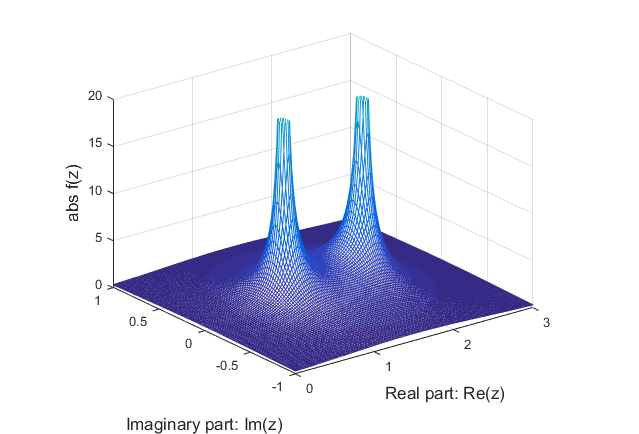
\includegraphics[width=0.75\textwidth]{figures/anum.png} % Replace with your image file
    \end{figure}
    
    \vspace{2cm}
    % {\Large \textbf{Analysis of Mass and Energy Balances in Copper Flash Smelting Furnaces}} \\
    % \vspace{3cm}
    
    % Personal information
    \begin{tabular}{rl}
    \large Name: & \large Alif Zaicho Nur Ahmad \begin{CJK}{UTF8}{gbsn}安曼迪\end{CJK} \\
    \large Student ID: & \large 243519015 \\
    \large Subject: & \large Numerical Analysis \\
    % \large Email: & \large \href{mailto:alifzaicho@csu.cn.edu}{\textcolor{blue}{alifzaicho@csu.cn.edu}} \\
    % \large Source Code & \large \href{https://www.github.com/alifzaicho}{\textcolor{blue}{github.com/alifzaicho}}\\
    \large Email: & \large \href{mailto:alifzaicho@csu.cn.edu}{alifzaicho@csu.cn.edu} \\
    \large Source Code & \large \href{https://github.com/alifzaicho/CSU-Numerical_Analysis_Spring_2025/tree/39201f506c1db20ce838fc36e13b952caa364c93}{github.com/alifzaicho/CSU-Numerical\_Analysis\_Spring\_2025}\\
    \large School: & \large School of Metallurgy and Environment \\
    \large University: & \large Central South University \\
    \large Date: & \large \today \\
    \end{tabular}
  \end{center}
  \clearpage
}

\begin{document}
\def\imagewidth{1}
\def\imagewidthone{0.75}
\makecover % Insert cover page
\tableofcontents

\section{Interpolation}
\subsection{Real Case: Interpolation of the normal distribution}

In mineral processing, the feed grade (concentration of valuable mineral) of an ore varies with the particle size distribution (PSD). The PSD is modeled using a normal distribution:
\begin{equation}
f(x \mid \mu, \sigma^2) = \frac{1}{\sqrt{2\pi\sigma^2}} 
e^{-\frac{(x - \mu)^2}{2\sigma^2}}
\end{equation}
where \( x \) is the particle size (in micrometers), \(\mu\) is the mean size, and \(\sigma\) is the standard deviation.

\subsection{General Polynomials}

The monomial basis functions are defined as:
\begin{equation}
P_i(x) = x^i
\end{equation}

A general polynomial of degree $ n $ is given by:
\begin{equation}
S_n(x) = a_0 + a_1 x + a_2 x^2 + \cdots + a_n x^n
\end{equation}

The entries of the Hilbert matrix \( H \) are computed as inner products:
\begin{equation}
H_{i,j} = \int_{a}^{b} x^{i+j} dx = \frac{b^{i+j+1} - a^{i+j+1}}{i+j+1}
\end{equation}

The entries of the d vector are computed as projections of \( f(x) \) onto the basis functions:
\begin{equation}
d_i = \int_{a}^{b} f(x) x^i dx
\end{equation}

The normal equations to solve are:
\begin{equation}
H \cdot \mathbf{a} = d
\end{equation}
where \( H \) is the Hilbert matrix, \( \mathbf{a} \) is the vector of coefficients to find, and \( d \) is the vector of projections.

\subsubsection{Algorithm}
\begin{algorithm}[H]
\caption{Monomial Basis Approximation}\label{alg:monomial}
\begin{algorithmic}
\Require Function $f$, degree $n$, interval $[a, b]$
\Ensure Coefficients $\mathbf{a}$ for the monomial approximation
\State \textbf{Form the Hilbert matrix $H$}:
\For{$i = 0$ to $n$}
    \For{$j = 0$ to $n$}
        \State Compute inner product: $H[i][j] \gets \int_{a}^{b} x^{i+j} dx$
        \State This forms the Hilbert matrix with entries $H_{i,j} = \langle x^i, x^j \rangle$
    \EndFor
\EndFor
\State \textbf{Construct the d vector}:
\For{$i = 0$ to $n$}
    \State Compute projection: $d[i] \gets \int_{a}^{b} f(x) x^{i} dx$
    \State This forms the vector $d$ with entries $d_i = \langle f(x), x^i \rangle$
\EndFor
\State \textbf{Solve the normal equations}:
\State Solve the linear system $H \cdot \mathbf{a} = d$ for coefficients $\mathbf{a}$
\State \textbf{return} $\mathbf{a}$
\end{algorithmic}
\end{algorithm}

\subsubsection{Python snippet for General polynomials}
\begin{lstlisting}[caption={Monomial Interpolation}, label=code:monointerpolation]
import numpy as np
from scipy.integrate import quad

def monomial_interpolation(func, degree, lower=-1, upper=1):
    """
    Compute monomial interpolation coefficients for the given function.
    
    Args:
        func: Function to approximate
        degree: Degree of the interpolating polynomial
        lower: Lower bound of the interval
        upper: Upper bound of the interval
        
    Returns:
        coeff: Coefficients of the interpolating polynomial
    """
    # Build the matrix and right-hand side vector
    A = np.zeros((degree + 1, degree + 1))
    Y = np.zeros(degree + 1)
    
    for i in range(degree + 1):
        for j in range(degree + 1):
            integrand = lambda x: x**i * x**j
            A[i, j], _ = quad(integrand, lower, upper)
        integrand = lambda x: func(x) * x**i
        Y[i], _ = quad(integrand, lower, upper)
    
    # Solve for coefficients
    coeff = np.linalg.solve(A, Y)
    return coeff

# Example usage:
def test_function(x):
    return (1/np.sqrt(2*np.pi))*np.exp((-x**2)/2)

coefficients = monomial_interpolation(test_function, degree=3, lower=-1, upper=1)
print("Interpolation coefficients:", coefficients)
\end{lstlisting}



\subsubsection{Results}

The Hilbert matrix \( H \) for degree 6 is formed as follows:
\[
H = \begin{bmatrix}
7 & 0 & 28.58 & 0 & 210.09 & 0 & 1838.27 \\
0 & 28.58 & 0 & 210.09 & 0 & 1838.27 & 0 \\
28.58 & 0 & 210.09 & 0 & 1838.27 & 0 & 17514.59 \\
0 & 210.09 & 0 & 1838.27 & 0 & 17514.59 & 0 \\
210.09 & 0 & 1838.27 & 0 & 17514.59 & 0 & 175543.92 \\
0 & 1838.27 & 0 & 17514.59 & 0 & 175543.92 & 0 \\
1838.27 & 0 & 17514.59 & 0 & 175543.92 & 0 & 1819580.27
\end{bmatrix}
\]

The vector \( d \) is constructed as:
\[
d^T = \begin{bmatrix}
1.00 & 0 & 0.99 & 0 & 2.91 & 0 & 13.61
\end{bmatrix}
\]

The resulting coefficients are:
\[
\mathbf{a}^T = \begin{bmatrix}
0.38 & 0 & -0.15 & 0 & 0.02 & 0 & 0.00
\end{bmatrix}
\]

Using the resulting coefficients, the approximated polynomial is:
\begin{equation}
p(x) = 0.38 + (-0.15)x^2 + 0.02x^4
\end{equation}

\begin{figure}[H]
    \centering
    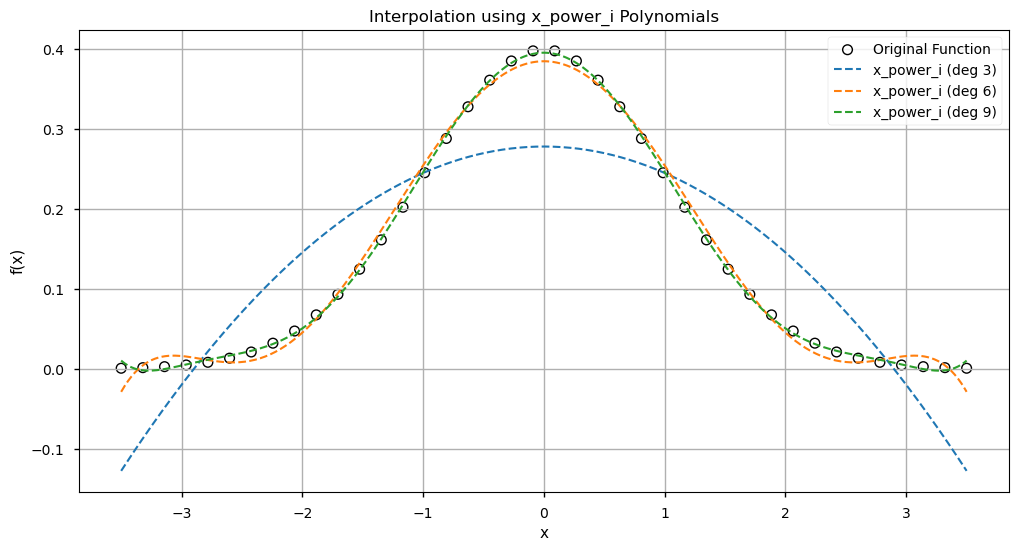
\includegraphics[width=\imagewidth\textwidth]{figures/02_interpolation/interpolation_method_x_power_i.png}
    \caption{Interpolation method using general polynomials}
\end{figure}
\begin{figure}[H]
    \centering
    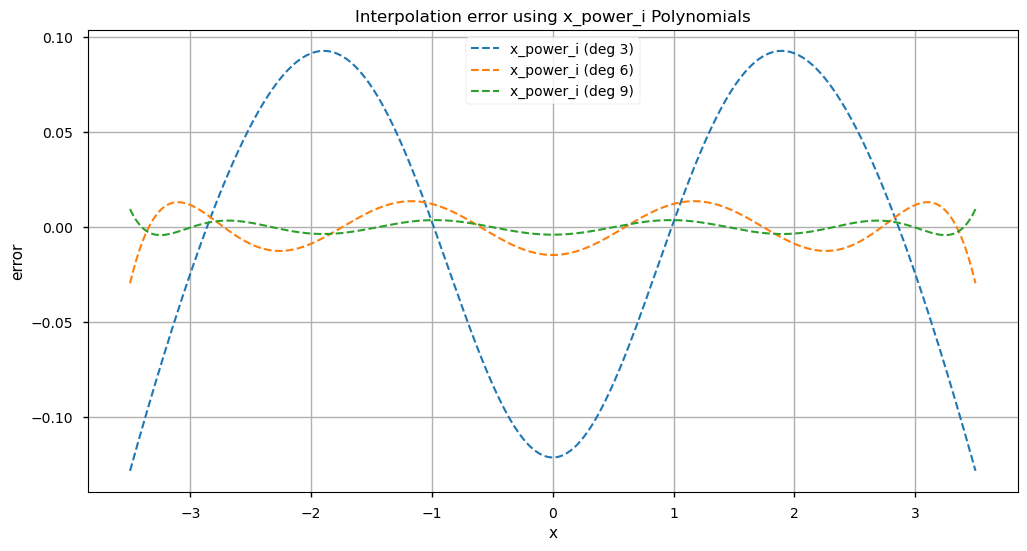
\includegraphics[width=\imagewidth\textwidth]{figures/02_interpolation/interpolation_error_method_x_power_i.png}
    \caption{Interpolation error from general polynomials}
\end{figure}

\subsubsection{Key Observations}
\begin{itemize}
    \item The Hilbert matrix \( H \) is symmetric and has a banded structure with alternating zero and non-zero entries.
    \item The vector \( d \) alternates between non-zero and zero values.
    \item The resulting coefficients \( \mathbf{a} \) also alternate between non-zero and zero values, aligning with the structure of \( H \) and \( d \).
    \item Even-indexed coefficients (0, 2, 4, 6) are non-zero, while odd-indexed coefficients (1, 3, 5) are zero.
\end{itemize}


\subsection{Legendre Polynomials}

The Legendre polynomials are defined as:
\begin{equation}
P_i(x) = \frac{1}{2^i i!} \frac{d^i}{dx^i} \left[ (x^2 - 1)^i \right]
\end{equation}

A general polynomial of degree $ n $ using Legendre polynomials is given by:
\begin{equation}
p_n(x) = a_0 P_0(x) + a_1 P_1(x) + a_2 P_2(x) + \cdots + a_n P_n(x)
\end{equation}

The weight function for Legendre polynomials is typically 1, which simplifies the integration process. This is because Legendre polynomials are orthogonal over the interval \([-1, 1]\) with respect to the weight function \(w(x) = 1\). The entries of the Hilbert matrix \( H \) for Legendre polynomials are computed as inner products:
\begin{equation}
H_{i,j} = \int_{-1}^{1} P_i(x) P_j(x) dx = \frac{2}{2i+1} \delta_{ij}
\end{equation}

The entries of the d vector are computed as projections of \( f(x) \) onto the Legendre polynomials:
\begin{equation}
d_i = \int_{-1}^{1} f(x) P_i(x) dx
\end{equation}

The normal equations to solve are:
\begin{equation}
H \cdot \mathbf{a} = d
\end{equation}
where \( H \) is the Hilbert matrix, \( \mathbf{a} \) is the vector of coefficients to find, and \( d \) is the vector of projections.

\subsubsection{Algorithm}
\begin{algorithm}[H]
\caption{Legendre Polynomial Approximation}\label{alg:legendre}
\begin{algorithmic}
\Require Function $f$, degree $n$, interval $[-1, 1]$
\Ensure Coefficients $\mathbf{a}$ for the Legendre approximation
\State \textbf{Form the Hilbert matrix $H$}:
\For{$i = 0$ to $n$}
    \For{$j = 0$ to $n$}
        \State Compute inner product: $H[i][j] \gets \int_{-1}^{1} P_i(x) P_j(x) dx$
        \State This forms the Hilbert matrix with entries $H_{i,j} = \langle P_i, P_j \rangle$
    \EndFor
\EndFor
\State \textbf{Construct the d vector}:
\For{$i = 0$ to $n$}
    \State Compute projection: $d[i] \gets \int_{-1}^{1} f(x) P_i(x) dx$
    \State This forms the vector $d$ with entries $d_i = \langle f(x), P_i \rangle$
\EndFor
\State \textbf{Solve the normal equations}:
\State Solve the linear system $H \cdot \mathbf{a} = d$ for coefficients $\mathbf{a}$
\State \textbf{return} $\mathbf{a}$
\end{algorithmic}
\end{algorithm}

\subsubsection{Python snippet for Legendre polynomials}
\begin{lstlisting}[style=custompython][caption={Legendre polynomial interpolation}, label=code:legendre]
import numpy as np
from scipy.integrate import quad

class FunctionApproximator:
    @staticmethod
    def legendre_poly(degree, x):
        """Compute Legendre polynomial P_n(x)"""
        if degree == 0:
            return np.ones_like(x)
        elif degree == 1:
            return x
        else:
            Pn_prev = np.ones_like(x)
            Pn_curr = x
            for i in range(1, degree):
                Pn_new = ((2*i + 1)*x*Pn_curr - i*Pn_prev)/(i + 1)
                Pn_prev, Pn_curr = Pn_curr, Pn_new
            return Pn_curr

    def legendre_shifted(self, degree, x):
        """Compute shifted Legendre polynomial on arbitrary interval"""
        a, b = self.default_lower, self.default_upper
        t = (2*x - (a + b)) / (b - a)  # Map to [-1, 1]
        return FunctionApproximator.legendre_poly(degree, t)

    def compute_approximation(self, degree, poly_type="legendre"):
        """Compute approximation using Legendre polynomials"""
        lower, upper = self.default_lower, self.default_upper
        poly_func = self.legendre_shifted

        # Build coefficient matrix and right-hand side vector
        A = np.zeros((degree+1, degree+1))
        Y = np.zeros(degree+1)

        for i in range(degree+1):
            for j in range(degree+1):
                integrand = lambda x: poly_func(i, x)*poly_func(j, x)
                A[i,j], _ = quad(integrand, lower, upper)
            integrand = lambda x: self.func(x)*poly_func(i, x)
            Y[i], _ = quad(integrand, lower, upper)

        # Solve the linear system
        a = np.linalg.solve(A, Y)
        return a

# Example usage:
def test_function(x):
    return (1/np.sqrt(2*np.pi))*np.exp((-x**2)/2)

approx = FunctionApproximator(test_function)
coefficients = approx.compute_approximation(3)  # Get 3rd degree approximation
print("Approximation coefficients:", coefficients)
\end{lstlisting}

\subsubsection{Results}
The Hilbert matrix \( H \) for degree 6 using Legendre polynomials is formed as follows:
\[
H = \begin{bmatrix}
2 & 0 & 0 & 0 & 0 & 0 & 0 \\
0 & 0.67 & 0 & 0 & 0 & 0 & 0 \\
0 & 0 & 0.40 & 0 & 0 & 0 & 0 \\
0 & 0 & 0 & 0.29 & 0 & 0 & 0 \\
0 & 0 & 0 & 0 & 0.22 & 0 & 0 \\
0 & 0 & 0 & 0 & 0 & 0.18 & 0 \\
0 & 0 & 0 & 0 & 0 & 0 & 0.15
\end{bmatrix}
\]

The vector \( d \) is constructed as:
\[
d^T = \begin{bmatrix}
0.68 & 0 & -0.04 & 0 & 0.00 & 0 & 0.00
\end{bmatrix}
\]

The resulting coefficients are:
\[
\mathbf{a}^T = \begin{bmatrix}
0.34 & 0 & -0.11 & 0 & 0.01 & 0 & 0.00
\end{bmatrix}
\]

Using the resulting coefficients, the approximated polynomial is:
\begin{equation}
p(x) = 0.34 P_0(x) - 0.11 P_2(x) + 0.01 P_4(x)
\end{equation}




\begin{figure}[H]
    \centering
    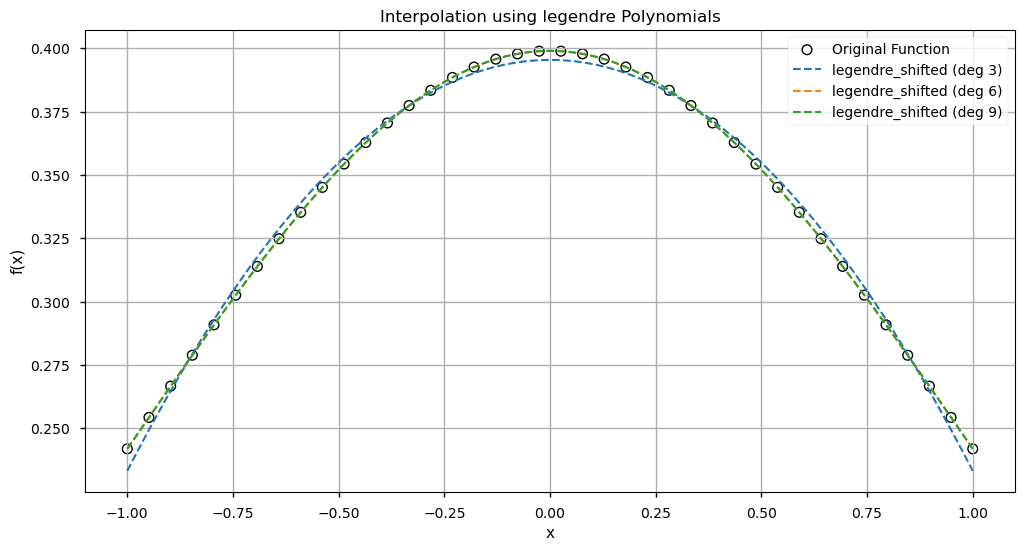
\includegraphics[width=\imagewidth\textwidth]{figures/02_interpolation/interpolation_method_legendre_shifted.png}
    \caption{Interpolation method using legendre polynomials}
\end{figure}

\begin{figure}[H]
    \centering
    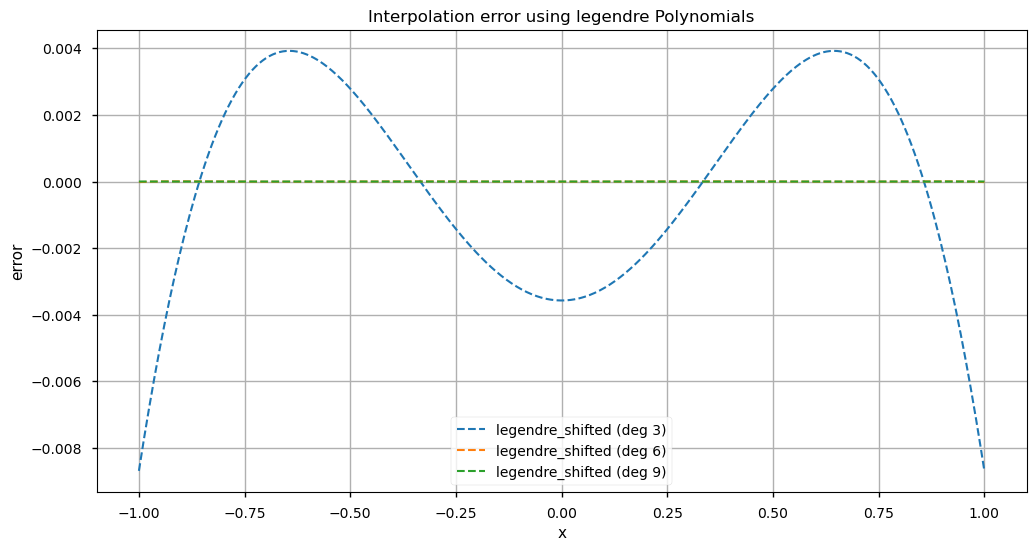
\includegraphics[width=\imagewidth\textwidth]{figures/02_interpolation/interpolation_error_method_legendre_shifted.png}
    \caption{Interpolation error from legendre polynomials}
\end{figure}


\subsubsection{Key Observations}
\begin{itemize}
    \item The Hilbert matrix \( H \) is diagonally dominant due to the orthogonality of Legendre polynomials.
    \item The vector \( d \) and the resulting coefficients \( \mathbf{a} \) have non-zero values at even indices, which aligns with the structure of \( H \).
    \item The orthogonality of Legendre polynomials simplifies the computation of the Hilbert matrix.
\end{itemize}

% \subsection{Chebyshev Polynomials}
\subsection{Chebyshev Polynomials Type 1}
The Chebyshev Type 1 polynomials are defined as:
\begin{equation}
T_i(x) = \cos(i \arccos(x))
\end{equation}

A general polynomial of degree $ n $ using Chebyshev Type 1 polynomials is given by:
\begin{equation}
p_n(x) = a_0 T_0(x) + a_1 T_1(x) + a_2 T_2(x) + \cdots + a_n T_n(x)
\end{equation}

The weight function for Chebyshev Type 1 polynomials is:
\begin{equation}
w(x) = \frac{1}{\sqrt{1-x^2}}
\end{equation}

The entries of the Hilbert matrix \( H \) for Chebyshev Type 1 polynomials are computed as inner products:
\begin{equation}
H_{i,j} = \int_{-1}^{1} T_i(x) T_j(x) \frac{1}{\sqrt{1-x^2}} dx
\end{equation}

The entries of the d vector are computed as projections of \( f(x) \) onto the Chebyshev Type 1 polynomials:
\begin{equation}
d_i = \int_{-1}^{1} f(x) T_i(x) \frac{1}{\sqrt{1-x^2}} dx
\end{equation}

The normal equations to solve are:
\begin{equation}
H \cdot \mathbf{a} = d
\end{equation}
where \( H \) is the Hilbert matrix, \( \mathbf{a} \) is the vector of coefficients to find, and \( d \) is the vector of projections.

\subsubsection{Algorithm}
\begin{algorithm}[H]
\caption{Chebyshev Type 1 Polynomial Approximation}\label{alg:chebyshev1}
\begin{algorithmic}
\Require Function $f$, degree $n$, interval $[-1, 1]$
\Ensure Coefficients $\mathbf{a}$ for the Chebyshev Type 1 approximation
\State \textbf{Form the Hilbert matrix $H$}:
\For{$i = 0$ to $n$}
    \For{$j = 0$ to $n$}
        \State Compute inner product: $H[i][j] \gets \int_{-1}^{1} T_i(x) T_j(x) \frac{1}{\sqrt{1-x^2}} dx$
        \State This forms the Hilbert matrix with entries $H_{i,j} = \langle T_i, T_j \rangle$
    \EndFor
\EndFor
\State \textbf{Construct the d vector}:
\For{$i = 0$ to $n$}
    \State Compute projection: $d[i] \gets \int_{-1}^{1} f(x) T_i(x) \frac{1}{\sqrt{1-x^2}} dx$
    \State This forms the vector $d$ with entries $d_i = \langle f(x), T_i \rangle$
\EndFor
\State \textbf{Solve the normal equations}:
\State Solve the linear system $H \cdot \mathbf{a} = d$ for coefficients $\mathbf{a}$
\State \textbf{return} $\mathbf{a}$
\end{algorithmic}
\end{algorithm}

\subsubsection{Python snippet for Chebyshev polynomials type 1}
\begin{lstlisting}[style=custompython][caption={Chebyshev polynomial type 1 interpolation}, label=code:cheby1]
import numpy as np
from scipy.integrate import quad

class FunctionApproximator:
    @staticmethod
    def chebyshev_1_poly(degree, x):
        """Chebyshev polynomial of the first kind T_n(x)"""
        if degree == 0:
            return np.ones_like(x)
        elif degree == 1:
            return x
        else:
            T_prev = np.ones_like(x)
            T_curr = x
            for i in range(1, degree):
                T_new = 2 * x * T_curr - T_prev
                T_prev, T_curr = T_curr, T_new
            return T_curr

    def chebyshev_1_shifted(self, degree, x):
        """Shifted Chebyshev polynomial of the first kind"""
        a, b = self.default_lower, self.default_upper
        t = (2 * x - (a + b)) / (b - a)  # Map to [-1, 1]
        return self.chebyshev_1_poly(degree, t)

    @staticmethod
    def weight_function(poly_type, x):
        """Weight functions for different polynomial types"""
        if poly_type == "chebyshev_1":
            return 1 / np.sqrt(1 - x**2 + 1e-12)  # Type 1 weight

    def compute_approximation(self, degree, poly_type="chebyshev_1"):
        """Compute approximation using Chebyshev Type 1 polynomials"""
        lower, upper = self.default_lower, self.default_upper
        poly_func = self.chebyshev_1_shifted

        # Build coefficient matrix and right-hand side vector
        A = np.zeros((degree+1, degree+1))
        Y = np.zeros(degree+1)

        for i in range(degree+1):
            for j in range(degree+1):
                integrand = lambda x: (poly_func(i, x) * poly_func(j, x) * 
                                      FunctionApproximator.weight_function(poly_type, x))
                A[i,j], _ = quad(integrand, lower, upper)
            integrand = lambda x: (self.func(x) * poly_func(i, x) *
                                  FunctionApproximator.weight_function(poly_type, x))
            Y[i], _ = quad(integrand, lower, upper)

        a = np.linalg.solve(A, Y)
        return a

# Example usage for Chebyshev Type 1
def test_function(x):
    return (1/np.sqrt(2*np.pi))*np.exp((-x**2)/2)

approx = FunctionApproximator(test_function)
type1_coeffs = approx.compute_approximation(5, 'chebyshev_1')
print("Chebyshev Type 1 coefficients:", type1_coeffs)
\end{lstlisting}

\subsubsection{Results}

For Chebyshev Type 1 polynomials, the Hilbert matrix \( H \) for degree 6 is:
\[
H = \begin{bmatrix}
3.14 & 0 & 0 & 0 & 0 & 0 & 0 \\
0 & 1.57 & 0 & 0 & 0 & 0 & 0 \\
0 & 0 & 1.57 & 0 & 0 & 0 & 0 \\
0 & 0 & 0 & 1.57 & 0 & 0 & 0 \\
0 & 0 & 0 & 0 & 1.57 & 0 & 0 \\
0 & 0 & 0 & 0 & 0 & 1.57 & 0 \\
0 & 0 & 0 & 0 & 0 & 0 & 1.57
\end{bmatrix}
\]

The vector \( d \) is constructed as:
\[
d^T = \begin{bmatrix}
0.99 & 0 & -0.12 & 0 & 0.01 & 0 & 0.00
\end{bmatrix}
\]

The resulting coefficients are:
\[
\mathbf{a}^T = \begin{bmatrix}
0.32 & 0 & -0.08 & 0 & 0.00 & 0 & 0.00
\end{bmatrix}
\]

Using the resulting coefficients, the approximated polynomial is:
\begin{equation}
p(x) = 0.32 T_0(x) - 0.08 T_2(x)
\end{equation}

\subsection{Chebyshev Polynomials Type 2}
The Chebyshev Type 2 polynomials are defined as:
\begin{equation}
U_i(x) = \frac{\sin((i+1) \arccos(x))}{\sin(\arccos(x))}
\end{equation}

A general polynomial of degree $ n $ using Chebyshev Type 2 polynomials is given by:
\begin{equation}
p_n(x) = a_0 U_0(x) + a_1 U_1(x) + a_2 U_2(x) + \cdots + a_n U_n(x)
\end{equation}

The weight function for Chebyshev Type 2 polynomials is:
\begin{equation}
w(x) = \sqrt{1-x^2}
\end{equation}

The entries of the Hilbert matrix \( H \) for Chebyshev Type 2 polynomials are computed as inner products:
\begin{equation}
H_{i,j} = \int_{-1}^{1} U_i(x) U_j(x) \sqrt{1-x^2} dx
\end{equation}

The entries of the d vector are computed as projections of \( f(x) \) onto the Chebyshev Type 2 polynomials:
\begin{equation}
d_i = \int_{-1}^{1} f(x) U_i(x) \sqrt{1-x^2} dx
\end{equation}

The normal equations to solve are:
\begin{equation}
H \cdot \mathbf{a} = d
\end{equation}
where \( H \) is the Hilbert matrix, \( \mathbf{a} \) is the vector of coefficients to find, and \( d \) is the vector of projections.

\subsubsection{Algorithm}
\begin{algorithm}[H]
\caption{Chebyshev Type 2 Polynomial Approximation}\label{alg:chebyshev2}
\begin{algorithmic}
\Require Function $f$, degree $n$, interval $[-1, 1]$
\Ensure Coefficients $\mathbf{a}$ for the Chebyshev Type 2 approximation
\State \textbf{Form the Hilbert matrix $H$}:
\For{$i = 0$ to $n$}
    \For{$j = 0$ to $n$}
        \State Compute inner product: $H[i][j] \gets \int_{-1}^{1} U_i(x) U_j(x) \sqrt{1-x^2} dx$
        \State This forms the Hilbert matrix with entries $H_{i,j} = \langle U_i, U_j \rangle$
    \EndFor
\EndFor
\State \textbf{Construct the d vector}:
\For{$i = 0$ to $n$}
    \State Compute projection: $d[i] \gets \int_{-1}^{1} f(x) U_i(x) \sqrt{1-x^2} dx$
    \State This forms the vector $d$ with entries $d_i = \langle f(x), U_i \rangle$
\EndFor
\State \textbf{Solve the normal equations}:
\State Solve the linear system $H \cdot \mathbf{a} = d$ for coefficients $\mathbf{a}$
\State \textbf{return} $\mathbf{a}$
\end{algorithmic}
\end{algorithm}

\subsubsection{Python snippet for Chebyshev polynomials type 2}
\begin{lstlisting}[style=custompython][caption={Chebyshev polynomial type 2 interpolation}, label=code:cheby2]
import numpy as np
from scipy.integrate import quad

class FunctionApproximator:
    @staticmethod
    def chebyshev_2_poly(degree, x):
        """Chebyshev polynomial of the second kind U_n(x)"""
        if degree == 0:
            return np.ones_like(x)
        elif degree == 1:
            return 2 * x
        else:
            U_prev = np.ones_like(x)
            U_curr = 2 * x
            for i in range(1, degree):
                U_new = 2 * x * U_curr - U_prev
                U_prev, U_curr = U_curr, U_new
            return U_curr

    def chebyshev_2_shifted(self, degree, x):
        """Shifted Chebyshev polynomial of the second kind"""
        a, b = self.default_lower, self.default_upper
        t = (2 * x - (a + b)) / (b - a)  # Map to [-1, 1]
        return self.chebyshev_2_poly(degree, t)

    @staticmethod
    def weight_function(poly_type, x):
        """Weight functions for different polynomial types"""
        if poly_type == "chebyshev_2":
            return np.sqrt(1 - x**2 + 1e-12)  # Type 2 weight

    def compute_approximation(self, degree, poly_type="chebyshev_2"):
        """Compute approximation using Chebyshev Type 2 polynomials"""
        lower, upper = self.default_lower, self.default_upper
        poly_func = self.chebyshev_2_shifted

        # Build coefficient matrix and right-hand side vector
        A = np.zeros((degree+1, degree+1))
        Y = np.zeros(degree+1)

        for i in range(degree+1):
            for j in range(degree+1):
                integrand = lambda x: (poly_func(i, x) * poly_func(j, x) * 
                                      FunctionApproximator.weight_function(poly_type, x))
                A[i,j], _ = quad(integrand, lower, upper)
            integrand = lambda x: (self.func(x) * poly_func(i, x) *
                                  FunctionApproximator.weight_function(poly_type, x))
            Y[i], _ = quad(integrand, lower, upper)

        a = np.linalg.solve(A, Y)
        return a

# Example usage for Chebyshev Type 2
def test_function(x):
    return (1/np.sqrt(2*np.pi))*np.exp((-x**2)/2)

approx = FunctionApproximator(test_function)
type2_coeffs = approx.compute_approximation(5, 'chebyshev_2')
print("Chebyshev Type 2 coefficients:", type2_coeffs)
\end{lstlisting}




\subsubsection{Results}


For Chebyshev Type 2 polynomials, the Hilbert matrix \( H \) for degree 6 is:
\[
H = \begin{bmatrix}
1.57 & 0 & 0 & 0 & 0 & 0 & 0 \\
0 & 1.57 & 0 & 0 & 0 & 0 & 0 \\
0 & 0 & 1.57 & 0 & 0 & 0 & 0 \\
0 & 0 & 0 & 1.57 & 0 & 0 & 0 \\
0 & 0 & 0 & 0 & 1.57 & 0 & 0 \\
0 & 0 & 0 & 0 & 0 & 1.57 & 0 \\
0 & 0 & 0 & 0 & 0 & 0 & 1.57
\end{bmatrix}
\]

The vector \( d \) is constructed as:
\[
d^T = \begin{bmatrix}
0.56 & 0 & -0.07 & 0 & 0.00 & 0 & 0.00
\end{bmatrix}
\]

The resulting coefficients are:
\[
\mathbf{a}^T = \begin{bmatrix}
0.35 & 0 & -0.04 & 0 & 0.00 & 0 & 0.00
\end{bmatrix}
\]

Using the resulting coefficients, the approximated polynomial is:
\begin{equation}
p(x) = 0.35 U_0(x) - 0.04 U_2(x)
\end{equation}




\begin{figure}[H]
    \centering
    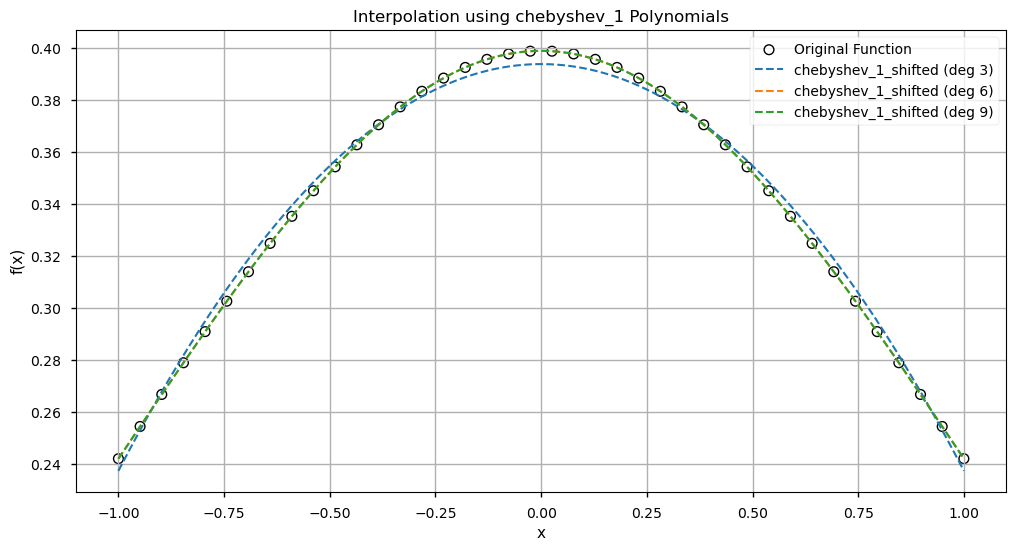
\includegraphics[width=\imagewidth\textwidth]{figures/02_interpolation/interpolation_method_chebyshev_1_shifted.png}
    \caption{Interpolation method using chebyshev polynomials type 1}
\end{figure}

\begin{figure}[H]
    \centering
    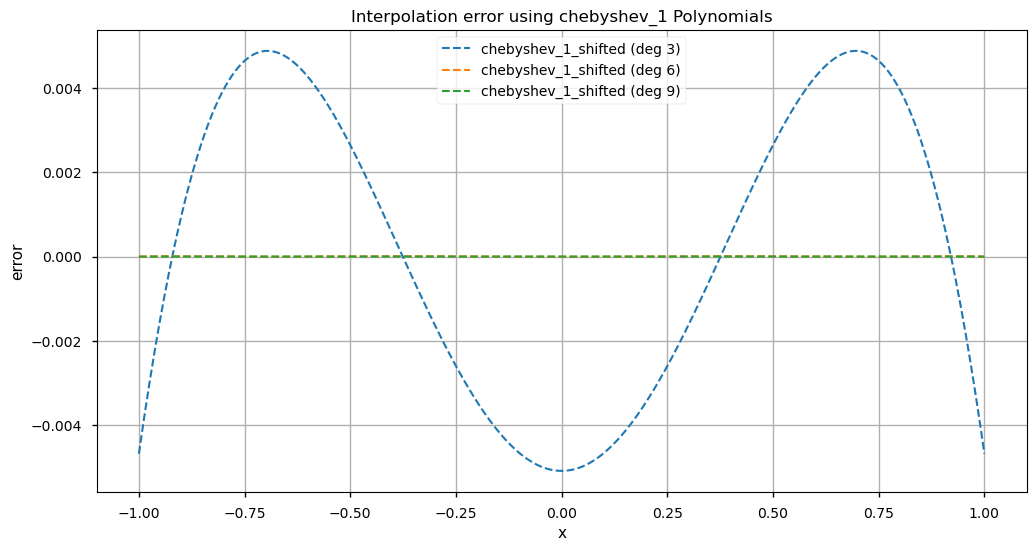
\includegraphics[width=\imagewidth\textwidth]{figures/02_interpolation/interpolation_error_method_chebyshev_1_shifted.png}
    \caption{Interpolation error from chebyshev polynomials type 1}
\end{figure}

\begin{figure}[H]
    \centering
    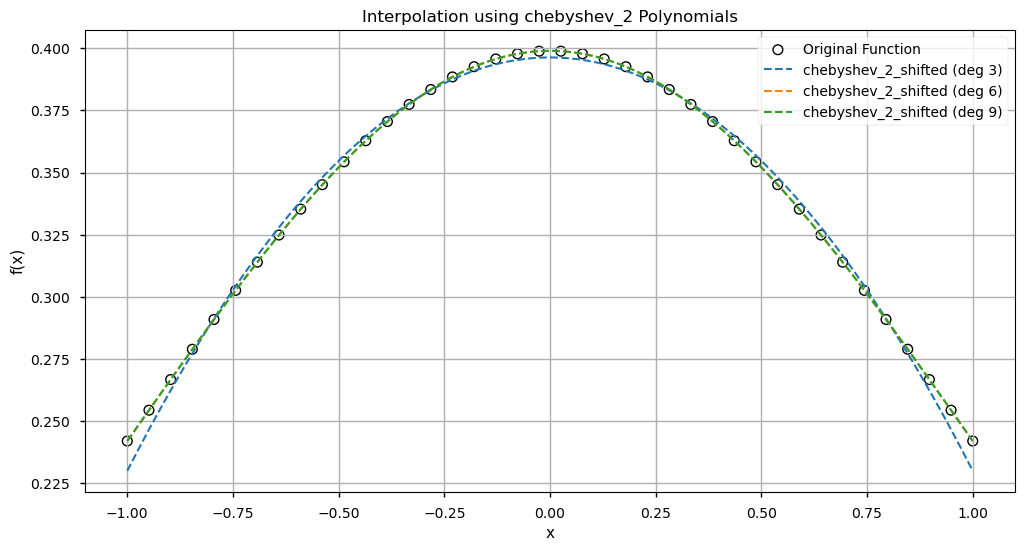
\includegraphics[width=\imagewidth\textwidth]{figures/02_interpolation/interpolation_method_chebyshev_2_shifted.png}
    \caption{Interpolation method using chebyshev polynomials type 2}
\end{figure}

\begin{figure}[H]
    \centering
    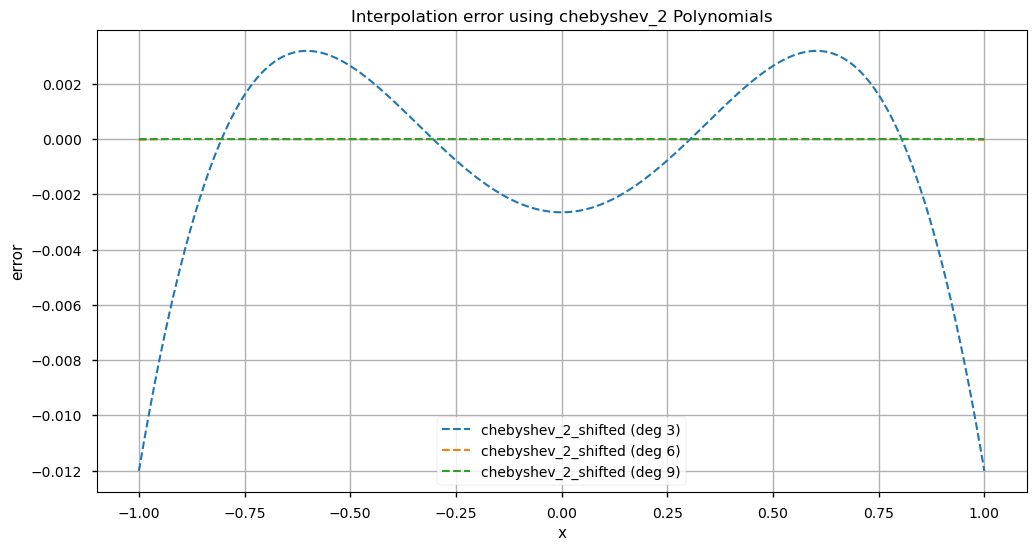
\includegraphics[width=\imagewidth\textwidth]{figures/02_interpolation/interpolation_error_method_chebyshev_2_shifted.png}
    \caption{Interpolation error from chebyshev polynomials type 2}
\end{figure}

\subsubsection{Key Observations}
\begin{itemize}
    \item The Hilbert matrices for both Chebyshev Type 1 and Type 2 polynomials are diagonally dominant.
    \item The vectors \( d \) and the resulting coefficients \( \mathbf{a} \) have non-zero values at even indices for both types of polynomials.
    \item The orthogonality of Chebyshev polynomials simplifies the computation of the Hilbert matrix.
\end{itemize}

\subsection{Laguerre Polynomials}

The Laguerre polynomials are defined as:
\begin{equation}
L_i(x) = \frac{e^x}{i!} \frac{d^i}{dx^i} \left( e^{-x} x^i \right)
\end{equation}

A general polynomial of degree $ n $ using Laguerre polynomials is given by:
\begin{equation}
p_n(x) = a_0 L_0(x) + a_1 L_1(x) + a_2 L_2(x) + \cdots + a_n L_n(x)
\end{equation}

The weight function for Laguerre polynomials is:
\begin{equation}
w(x) = e^{-x}
\end{equation}

The entries of the Hilbert matrix \( H \) for Laguerre polynomials are computed as inner products:
\begin{equation}
H_{i,j} = \int_{0}^{\infty} L_i(x) L_j(x) e^{-x} dx
\end{equation}

The entries of the d vector are computed as projections of \( f(x) \) onto the Laguerre polynomials:
\begin{equation}
d_i = \int_{0}^{\infty} f(x) L_i(x) e^{-x} dx
\end{equation}

The normal equations to solve are:
\begin{equation}
H \cdot \mathbf{a} = d
\end{equation}
where \( H \) is the Hilbert matrix, \( \mathbf{a} \) is the vector of coefficients to find, and \( d \) is the vector of projections.

\subsubsection{Algorithm}
\begin{algorithm}[H]
\caption{Laguerre Polynomial Approximation}\label{alg:laguerre}
\begin{algorithmic}
\Require Function $f$, degree $n$, interval $[0, \infty)$
\Ensure Coefficients $\mathbf{a}$ for the Laguerre approximation
\State \textbf{Form the Hilbert matrix $H$}:
\For{$i = 0$ to $n$}
    \For{$j = 0$ to $n$}
        \State Compute inner product: $H[i][j] \gets \int_{0}^{\infty} L_i(x) L_j(x) e^{-x} dx$
        \State This forms the Hilbert matrix with entries $H_{i,j} = \langle L_i, L_j \rangle$
    \EndFor
\EndFor
\State \textbf{Construct the d vector}:
\For{$i = 0$ to $n$}
    \State Compute projection: $d[i] \gets \int_{0}^{\infty} f(x) L_i(x) e^{-x} dx$
    \State This forms the vector $d$ with entries $d_i = \langle f(x), L_i \rangle$
\EndFor
\State \textbf{Solve the normal equations}:
\State Solve the linear system $H \cdot \mathbf{a} = d$ for coefficients $\mathbf{a}$
\State \textbf{return} $\mathbf{a}$
\end{algorithmic}
\end{algorithm}
\subsubsection{Python snippet for Laguerre polynomials}
\begin{lstlisting}[style=custompython][caption={Laguerre polynomial interpolation}, label=code:laguerre]
import numpy as np
from scipy.integrate import quad

class FunctionApproximator:
    @staticmethod
    def laguerre_poly(degree, x):
        """Laguerre polynomial L_n(x)"""
        if degree == 0:
            return np.ones_like(x)
        elif degree == 1:
            return 1 - x
        else:
            L_prev = np.ones_like(x)
            L_curr = 1 - x
            for i in range(1, degree):
                L_new = ((2 * i + 1 - x) * L_curr - i * L_prev) / (i + 1)
                L_prev, L_curr = L_curr, L_new
            return L_curr

    @staticmethod
    def weight_function(poly_type, x):
        """Weight function for Laguerre polynomials"""
        if poly_type == "laguerre":
            return np.exp(-x)  # Laguerre weight function

    def compute_approximation(self, degree, poly_type="laguerre"):
        """Compute approximation using Laguerre polynomials"""
        lower, upper = 0, np.inf  # Laguerre polynomials are defined on [0, inf)
        
        # Build coefficient matrix and right-hand side vector
        A = np.zeros((degree+1, degree+1))
        Y = np.zeros(degree+1)

        for i in range(degree+1):
            for j in range(degree+1):
                integrand = lambda x: (FunctionApproximator.laguerre_poly(i, x) *
                                      FunctionApproximator.laguerre_poly(j, x) *
                                      FunctionApproximator.weight_function(poly_type, x))
                A[i,j], _ = quad(integrand, lower, upper)
            integrand = lambda x: (self.func(x) *
                                  FunctionApproximator.laguerre_poly(i, x) *
                                  FunctionApproximator.weight_function(poly_type, x))
            Y[i], _ = quad(integrand, lower, upper)

        a = np.linalg.solve(A, Y)
        return a

# Example usage for Laguerre polynomials
def test_function(x):
    return (1/np.sqrt(2*np.pi))*np.exp((-x**2)/2)

approx = FunctionApproximator(test_function)
laguerre_coeffs = approx.compute_approximation(5, 'laguerre')
print("Laguerre coefficients:", laguerre_coeffs)
\end{lstlisting}

\subsubsection{Results}

For Laguerre polynomials, the Hilbert matrix \( H \) for degree 6 is:
\[
H = \begin{bmatrix}
1 & 0 & 0 & 0 & 0 & 0 & 0 \\
0 & 1 & 0 & 0 & 0 & 0 & 0 \\
0 & 0 & 1 & 0 & 0 & 0 & 0 \\
0 & 0 & 0 & 1 & 0 & 0 & 0 \\
0 & 0 & 0 & 0 & 1 & 0 & 0 \\
0 & 0 & 0 & 0 & 0 & 1 & 0 \\
0 & 0 & 0 & 0 & 0 & 0 & 1
\end{bmatrix}
\]

The vector \( d \) is constructed as:
\[
d^T = \begin{bmatrix}
0.26 & 0.12 & 0.05 & 0.01 & -0.01 & -0.01 & -0.01
\end{bmatrix}
\]

The resulting coefficients are:
\[
\mathbf{a}^T = \begin{bmatrix}
0.26 & 0.12 & 0.05 & 0.01 & -0.01 & -0.01 & -0.01
\end{bmatrix}
\]

Using the resulting coefficients, the approximated polynomial is:
\begin{equation}
p(x) = 0.26 L_0(x) + 0.12 L_1(x) + 0.05 L_2(x) + 0.01 L_3(x) - 0.01 L_4(x) - 0.01 L_5(x) - 0.01 L_6(x)
\end{equation}


\begin{figure}[H]
    \centering
    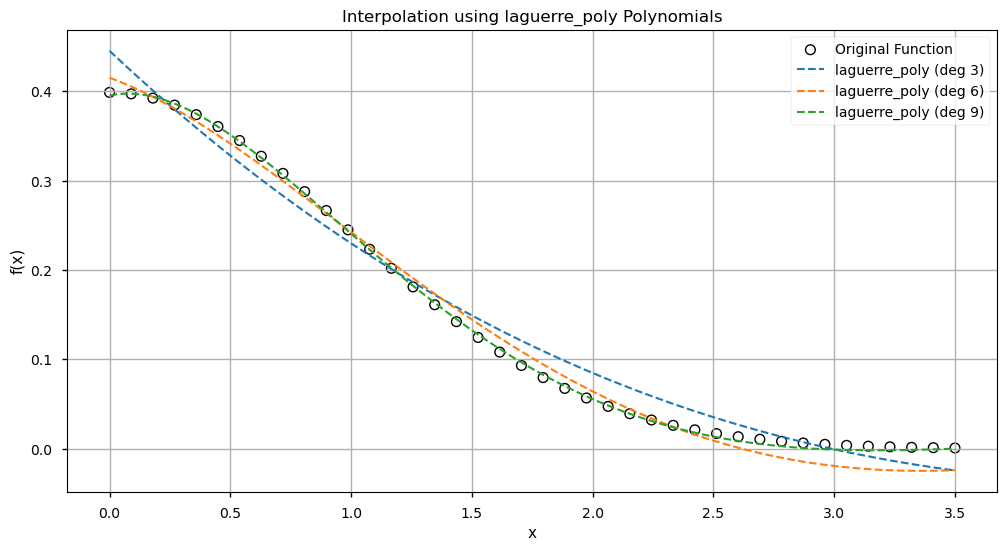
\includegraphics[width=\imagewidth\textwidth]{figures/02_interpolation/interpolation_method_laguerre_poly.png}
    \caption{Interpolation method using laguerre polynomials}
\end{figure}

\begin{figure}[H]
    \centering
    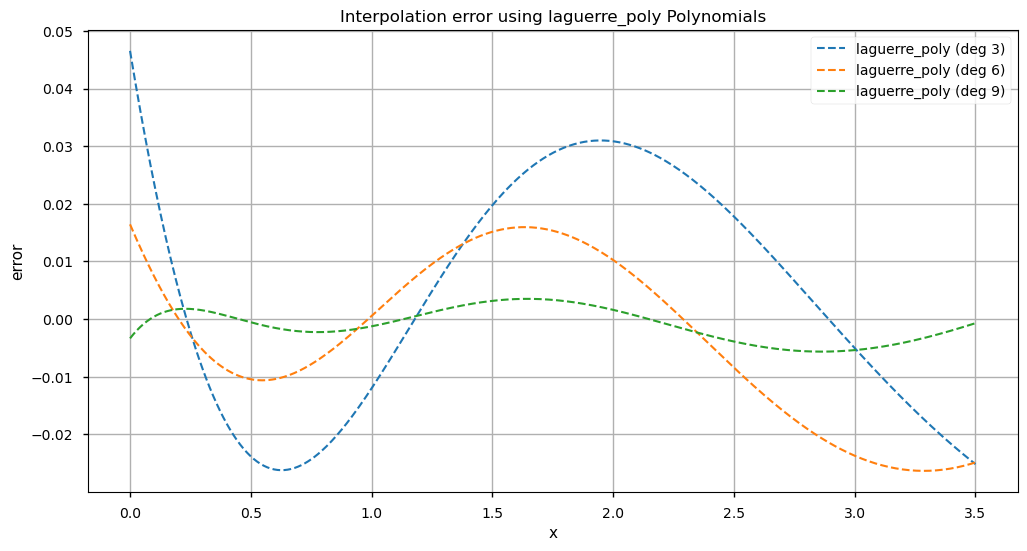
\includegraphics[width=\imagewidth\textwidth]{figures/02_interpolation/interpolation_error_method_laguerre_poly.png}
    \caption{Interpolation error from laguerre polynomials}
\end{figure}

\subsubsection{Key Observations}
\begin{itemize}
    \item The Hilbert matrix \( H \) is diagonal due to the orthogonality of Laguerre polynomials.
    \item The resulting coefficients \( \mathbf{a} \) match the structure of \( H \) and \( d \).
    \item The orthogonality of Laguerre polynomials simplifies the computation of the Hilbert matrix.
\end{itemize}

\subsection{Hermite Polynomials}

The Hermite polynomials are defined as:
\begin{equation}
H_i(x) = (-1)^i e^{x^2} \frac{d^i}{dx^i} \left( e^{-x^2} \right)
\end{equation}

A general polynomial of degree $ n $ using Hermite polynomials is given by:
\begin{equation}
p_n(x) = a_0 H_0(x) + a_1 H_1(x) + a_2 H_2(x) + \cdots + a_n H_n(x)
\end{equation}

The weight function for Hermite polynomials is:
\begin{equation}
w(x) = e^{-x^2}
\end{equation}

The entries of the Hilbert matrix \( H \) for Hermite polynomials are computed as inner products:
\begin{equation}
H_{i,j} = \int_{-\infty}^{\infty} H_i(x) H_j(x) e^{-x^2} dx
\end{equation}

The entries of the d vector are computed as projections of \( f(x) \) onto the Hermite polynomials:
\begin{equation}
d_i = \int_{-\infty}^{\infty} f(x) H_i(x) e^{-x^2} dx
\end{equation}

The normal equations to solve are:
\begin{equation}
H \cdot \mathbf{a} = d
\end{equation}
where \( H \) is the Hilbert matrix, \( \mathbf{a} \) is the vector of coefficients to find, and \( d \) is the vector of projections.

\subsubsection{Algorithm}
\begin{algorithm}[H]
\caption{Hermite Polynomial Approximation}\label{alg:hermite}
\begin{algorithmic}
\Require Function $f$, degree $n$, interval $(-\infty, \infty)$
\Ensure Coefficients $\mathbf{a}$ for the Hermite approximation
\State \textbf{Form the Hilbert matrix $H$}:
\For{$i = 0$ to $n$}
    \For{$j = 0$ to $n$}
        \State Compute inner product: $H[i][j] \gets \int_{-\infty}^{\infty} H_i(x) H_j(x) e^{-x^2} dx$
        \State This forms the Hilbert matrix with entries $H_{i,j} = \langle H_i, H_j \rangle$
    \EndFor
\EndFor
\State \textbf{Construct the d vector}:
\For{$i = 0$ to $n$}
    \State Compute projection: $d[i] \gets \int_{-\infty}^{\infty} f(x) H_i(x) e^{-x^2} dx$
    \State This forms the vector $d$ with entries $d_i = \langle f(x), H_i \rangle$
\EndFor
\State \textbf{Solve the normal equations}:
\State Solve the linear system $H \cdot \mathbf{a} = d$ for coefficients $\mathbf{a}$
\State \textbf{return} $\mathbf{a}$
\end{algorithmic}
\end{algorithm}

\subsubsection{Results}

For Hermite polynomials, the Hilbert matrix \( H \) for degree 6 is:
\[
H = \begin{bmatrix}
1.77 & 0 & 0 & 0 & 0 & 0 & 0 \\
0 & 3.54 & 0 & 0 & 0 & 0 & 0 \\
0 & 0 & 14.18 & 0 & 0 & 0 & 0 \\
0 & 0 & 0 & 85.08 & 0 & 0 & 0 \\
0 & 0 & 0 & 0 & 680.62 & 0 & 0 \\
0 & 0 & 0 & 0 & 0 & 6806.22 & 0 \\
0 & 0 & 0 & 0 & 0 & 0 & 81674.67
\end{bmatrix}
\]

The vector \( d \) is constructed as:
\[
d^T = \begin{bmatrix}
0.58 & 0 & -0.38 & 0 & 0.77 & 0 & -2.57
\end{bmatrix}
\]

The resulting coefficients are:
\[
\mathbf{a}^T = \begin{bmatrix}
0.33 & 0 & -0.03 & 0 & 0.00 & 0 & 0.00
\end{bmatrix}
\]

Using the resulting coefficients, the approximated polynomial is:
\begin{equation}
p(x) = 0.33 H_0(x) - 0.03 H_2(x)
\end{equation}


\begin{figure}[H]
    \centering
    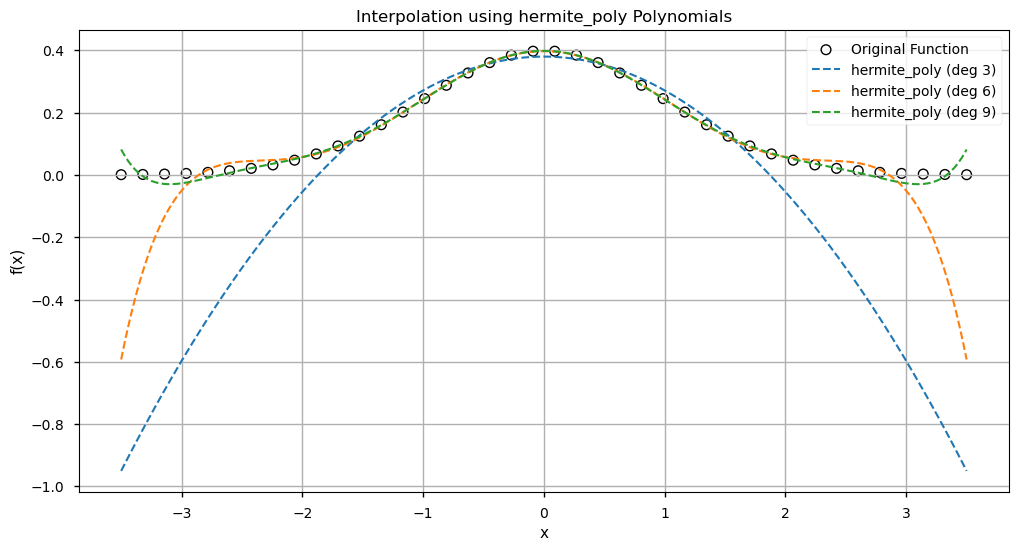
\includegraphics[width=\imagewidth\textwidth]{figures/02_interpolation/interpolation_method_hermite_poly.png}
    \caption{Interpolation method using hermite polynomials}
\end{figure}
\begin{figure}[H]
    \centering
    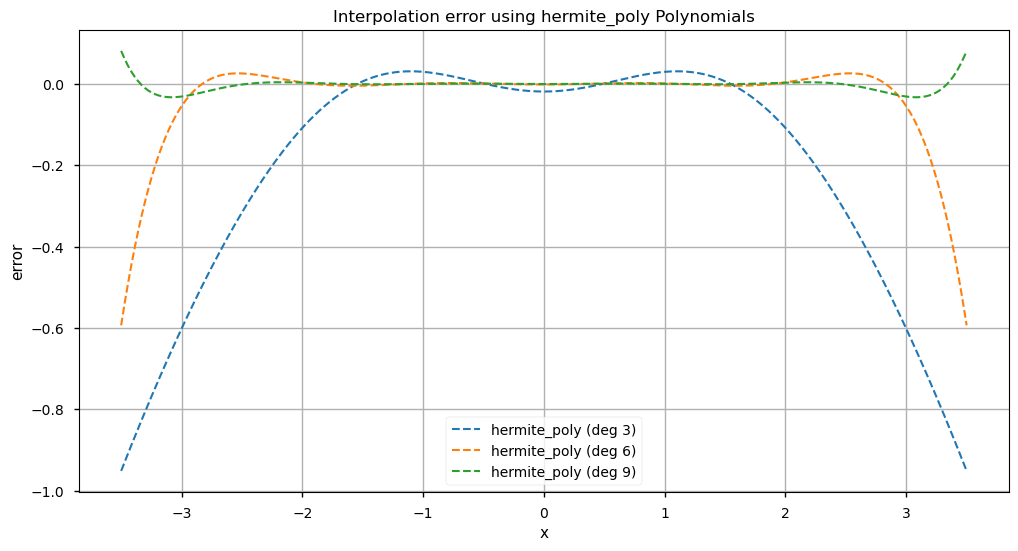
\includegraphics[width=\imagewidth\textwidth]{figures/02_interpolation/interpolation_error_method_hermite_poly.png}
    \caption{Interpolation error from hermite polynomials}
\end{figure}

\subsubsection{Python snippet for Hermite polynomials}
\begin{lstlisting}[style=custompython][caption={Hermite polynomial interpolation}, label=code:hermite]
import numpy as np
from scipy.integrate import quad

class FunctionApproximator:
    @staticmethod
    def hermite_poly(degree, x):
        """Hermite polynomial H_n(x)"""
        if degree == 0:
            return np.ones_like(x)
        elif degree == 1:
            return 2 * x
        else:
            H_prev = np.ones_like(x)
            H_curr = 2 * x
            for i in range(1, degree):
                H_new = 2 * x * H_curr - 2 * i * H_prev
                H_prev, H_curr = H_curr, H_new
            return H_curr

    @staticmethod
    def weight_function(poly_type, x):
        """Weight function for Hermite polynomials"""
        if poly_type == "hermite":
            return np.exp(-x**2)  # Hermite weight function

    def compute_approximation(self, degree, poly_type="hermite"):
        """Compute approximation using Hermite polynomials"""
        lower, upper = -np.inf, np.inf  # Hermite polynomials are defined on (-inf, inf)
        
        # Build coefficient matrix and right-hand side vector
        A = np.zeros((degree+1, degree+1))
        Y = np.zeros(degree+1)

        for i in range(degree+1):
            for j in range(degree+1):
                integrand = lambda x: (FunctionApproximator.hermite_poly(i, x) *
                                      FunctionApproximator.hermite_poly(j, x) *
                                      FunctionApproximator.weight_function(poly_type, x))
                A[i,j], _ = quad(integrand, lower, upper)
            integrand = lambda x: (self.func(x) *
                                  FunctionApproximator.hermite_poly(i, x) *
                                  FunctionApproximator.weight_function(poly_type, x))
            Y[i], _ = quad(integrand, lower, upper)

        a = np.linalg.solve(A, Y)
        return a

# Example usage for Hermite polynomials
def test_function(x):
    return (1/np.sqrt(2*np.pi))*np.exp((-x**2)/2)

approx = FunctionApproximator(test_function)
hermite_coeffs = approx.compute_approximation(5, 'hermite')
print("Hermite coefficients:", hermite_coeffs)
\end{lstlisting}

\subsubsection{Key Observations}
\begin{itemize}
    \item The Hilbert matrix \( H \) is diagonally dominant due to the orthogonality of Hermite polynomials.
    \item The resulting coefficients \( \mathbf{a} \) have non-zero values at even indices, which aligns with the structure of \( H \) and \( d \).
    \item The orthogonality of Hermite polynomials simplifies the computation of the Hilbert matrix.
\end{itemize}





\section{Least Square}
\subsection{Real Case: Mechanical Properties of Steel}
This study explores the relationship between steel composition, temperature conditions, and mechanical properties using least squares polynomial approximation. The dataset contains tension test results for various steel alloys tested under different temperatures. Our goal is to quantify how chemical elements and temperature influence critical mechanical properties: yield strength (YS), ultimate tensile strength (UTS), elongation (EL), and reduction of area (RA).

\begin{table}[htbp]
\centering
\caption{Sample Data from merged\_data.csv (Part 1)}
\label{tab:sample_data_part1}
\begin{tabular}{lrrrrrrrr}
\toprule
Sample & C (wt\%) & Si (wt\%) & Mn (wt\%) & P (wt\%) & S (wt\%) & Ni (wt\%) & Cr (wt\%) & Mo (wt\%) \\
\midrule
1 & 0.12 & 0.34 & 1.23 & 0.021 & 0.015 & 0.01 & 0.02 & 0.01 \\
2 & 0.20 & 0.45 & 1.45 & 0.023 & 0.018 & 0.01 & 0.02 & 0.01 \\
3 & 0.18 & 0.30 & 1.35 & 0.020 & 0.012 & 0.01 & 0.02 & 0.01 \\
4 & 0.25 & 0.50 & 1.50 & 0.025 & 0.020 & 0.01 & 0.02 & 0.01 \\
5 & 0.15 & 0.35 & 1.30 & 0.018 & 0.010 & 0.01 & 0.02 & 0.01 \\
6 & 0.22 & 0.40 & 1.40 & 0.022 & 0.016 & 0.01 & 0.02 & 0.01 \\
7 & 0.19 & 0.38 & 1.42 & 0.021 & 0.014 & 0.01 & 0.02 & 0.01 \\
8 & 0.24 & 0.48 & 1.55 & 0.024 & 0.019 & 0.01 & 0.02 & 0.01 \\
\bottomrule
\end{tabular}
\end{table}

\begin{table}[htbp]
\centering
\caption{Sample Data from merged\_data.csv (Part 2)}
\label{tab:sample_data_part2}
\begin{tabular}{lrrrrrrrr}
\toprule
Sample & Cu (wt\%) & Ti (wt\%) & Al (wt\%) & B (wt\%) & N (wt\%) & V (wt\%) & Co (wt\%) & Nb+Ta (wt\%) \\
\midrule
1 & 0.01 & 0.01 & 0.02 & 0.0025 & 0.005 & 0.01 & 0.01 & 0.01 \\
2 & 0.01 & 0.01 & 0.03 & 0.0030 & 0.006 & 0.01 & 0.01 & 0.01 \\
3 & 0.01 & 0.01 & 0.02 & 0.0020 & 0.004 & 0.01 & 0.01 & 0.01 \\
4 & 0.01 & 0.01 & 0.03 & 0.0035 & 0.007 & 0.01 & 0.01 & 0.01 \\
5 & 0.01 & 0.01 & 0.02 & 0.0022 & 0.004 & 0.01 & 0.01 & 0.01 \\
6 & 0.01 & 0.01 & 0.02 & 0.0028 & 0.005 & 0.01 & 0.01 & 0.01 \\
7 & 0.01 & 0.01 & 0.02 & 0.0026 & 0.005 & 0.01 & 0.01 & 0.01 \\
8 & 0.01 & 0.01 & 0.03 & 0.0032 & 0.006 & 0.01 & 0.01 & 0.01 \\
\bottomrule
\end{tabular}
\end{table}

\begin{table}[htbp]
\centering
\caption{Sample Data from merged\_data.csv (Part 3)}
\label{tab:sample_data_part3}
\begin{tabular}{lrrrrrrrr}
\toprule
Sample & Temperature (K) & YS (MPa) & UTS (MPa) & EL (\%) & RA (\%) \\
\midrule
1 & 298 & 450 & 620 & 25 & 60 \\
2 & 298 & 520 & 710 & 20 & 55 \\
3 & 373 & 410 & 580 & 30 & 70 \\
4 & 373 & 550 & 750 & 22 & 50 \\
5 & 448 & 380 & 550 & 35 & 75 \\
6 & 448 & 500 & 680 & 28 & 60 \\
7 & 523 & 350 & 520 & 40 & 80 \\
8 & 523 & 480 & 650 & 25 & 65 \\
\bottomrule
\end{tabular}
\end{table}


\begin{table}[htbp]
\centering
\caption{Summary Statistics for merged\_data.csv (Part 1)}
\label{tab:summary_stats_part1}
\begin{tabular}{lrrrrrr}
\toprule
Statistic & C (wt\%) & Si (wt\%) & Mn (wt\%) & P (wt\%) & S (wt\%) & Ni (wt\%) \\
\midrule
Count & 994 & 994 & 994 & 994 & 994 & 994 \\
Mean & 0.18 & 0.74 & 1.36 & 0.02 & 0.01 & 17.49 \\
Std Dev & 0.16 & 0.30 & 0.33 & 0.01 & 0.01 & 8.25 \\
Min & 0.04 & 0.22 & 0.48 & 0.01 & 0.00 & 8.79 \\
25\% & 0.06 & 0.54 & 1.12 & 0.02 & 0.01 & 12.06 \\
50\% & 0.07 & 0.62 & 1.47 & 0.02 & 0.01 & 13.21 \\
75\% & 0.37 & 0.92 & 1.60 & 0.02 & 0.01 & 21.42 \\
Max & 0.52 & 1.62 & 1.82 & 0.04 & 0.03 & 35.63 \\
\bottomrule
\end{tabular}
\end{table}

\begin{table}[htbp]
\centering
\caption{Summary Statistics for merged\_data.csv (Part 2)}
\label{tab:summary_stats_part2}
\begin{tabular}{lrrrrrr}
\toprule
Statistic & Cr (wt\%) & Mo (wt\%) & Cu (wt\%) & Ti (wt\%) & Al (wt\%) & B (wt\%) \\
\midrule
Count & 994 & 938 & 966 & 938 & 938 & 700 \\
Mean & 20.82 & 0.39 & 0.17 & 0.12 & 0.05 & 0.00 \\
Std Dev & 3.55 & 0.75 & 0.49 & 0.18 & 0.10 & 0.00 \\
Min & 16.42 & 0 & 0.01 & 0 & 0 & 0.00 \\
25\% & 17.86 & 0.03 & 0.05 & 0.01 & 0.00 & 0.00 \\
50\% & 18.70 & 0.07 & 0.07 & 0.02 & 0.01 & 0.00 \\
75\% & 24.90 & 0.25 & 0.12 & 0.06 & 0.04 & 0.00 \\
Max & 27.49 & 2.38 & 3.05 & 0.55 & 0.52 & 0.00 \\
\bottomrule
\end{tabular}
\end{table}

\begin{table}[htbp]
\centering
\caption{Summary Statistics for merged\_data.csv (Part 3)}
\label{tab:summary_stats_part3}
\begin{tabular}{lrrrrrr}
\toprule
Statistic & N (wt\%) & V (wt\%) & Co (wt\%) & Nb+Ta (wt\%) & Fe (wt\%) & Temperature (K) \\
\midrule
Count & 980 & 126 & 560 & 714 & 994 & 994 \\
Mean & 0.04 & 0.04 & 0.20 & 0.20 & 58.38 & 58.38 \\
Std Dev & 0.04 & 0.00 & 0.15 & 0.32 & 10.58 & 10.58 \\
Min & 0.01 & 0.03 & 0.00 & 0 & 34.31 & 34.31 \\
25\% & 0.02 & 0.03 & 0.04 & 0.01 & 51.05 & 51.05 \\
50\% & 0.03 & 0.03 & 0.23 & 0.01 & 64.84 & 64.84 \\
75\% & 0.05 & 0.04 & 0.31 & 0.46 & 66.57 & 66.57 \\
Max & 0.27 & 0.04 & 0.54 & 0.88 & 69.69 & 69.69 \\
\bottomrule
\end{tabular}
\end{table}

\begin{table}[htbp]
\centering
\caption{Summary Statistics for merged\_data.csv (Part 4)}
\label{tab:summary_stats_part4}
\begin{tabular}{lrrrrrr}
\toprule
Statistic & YS (MPa) & UTS (MPa) & EL (\%) & RA (\%) \\
\midrule
Count & 773 & 773 & 773 & 773 \\
Mean & 533.93 & 174.87 & 408.23 & 40.35 \\
Std Dev & 286.38 & 47.20 & 122.74 & 17.10 \\
Min & 25 & 35 & 20 & 8 \\
25\% & 300 & 148 & 337 & 29 \\
50\% & 575 & 171 & 436 & 40 \\
75\% & 750 & 200 & 488 & 47 \\
Max & 1000 & 342 & 711 & 128 \\
\bottomrule
\end{tabular}
\end{table}

\begin{figure}
    \centering
    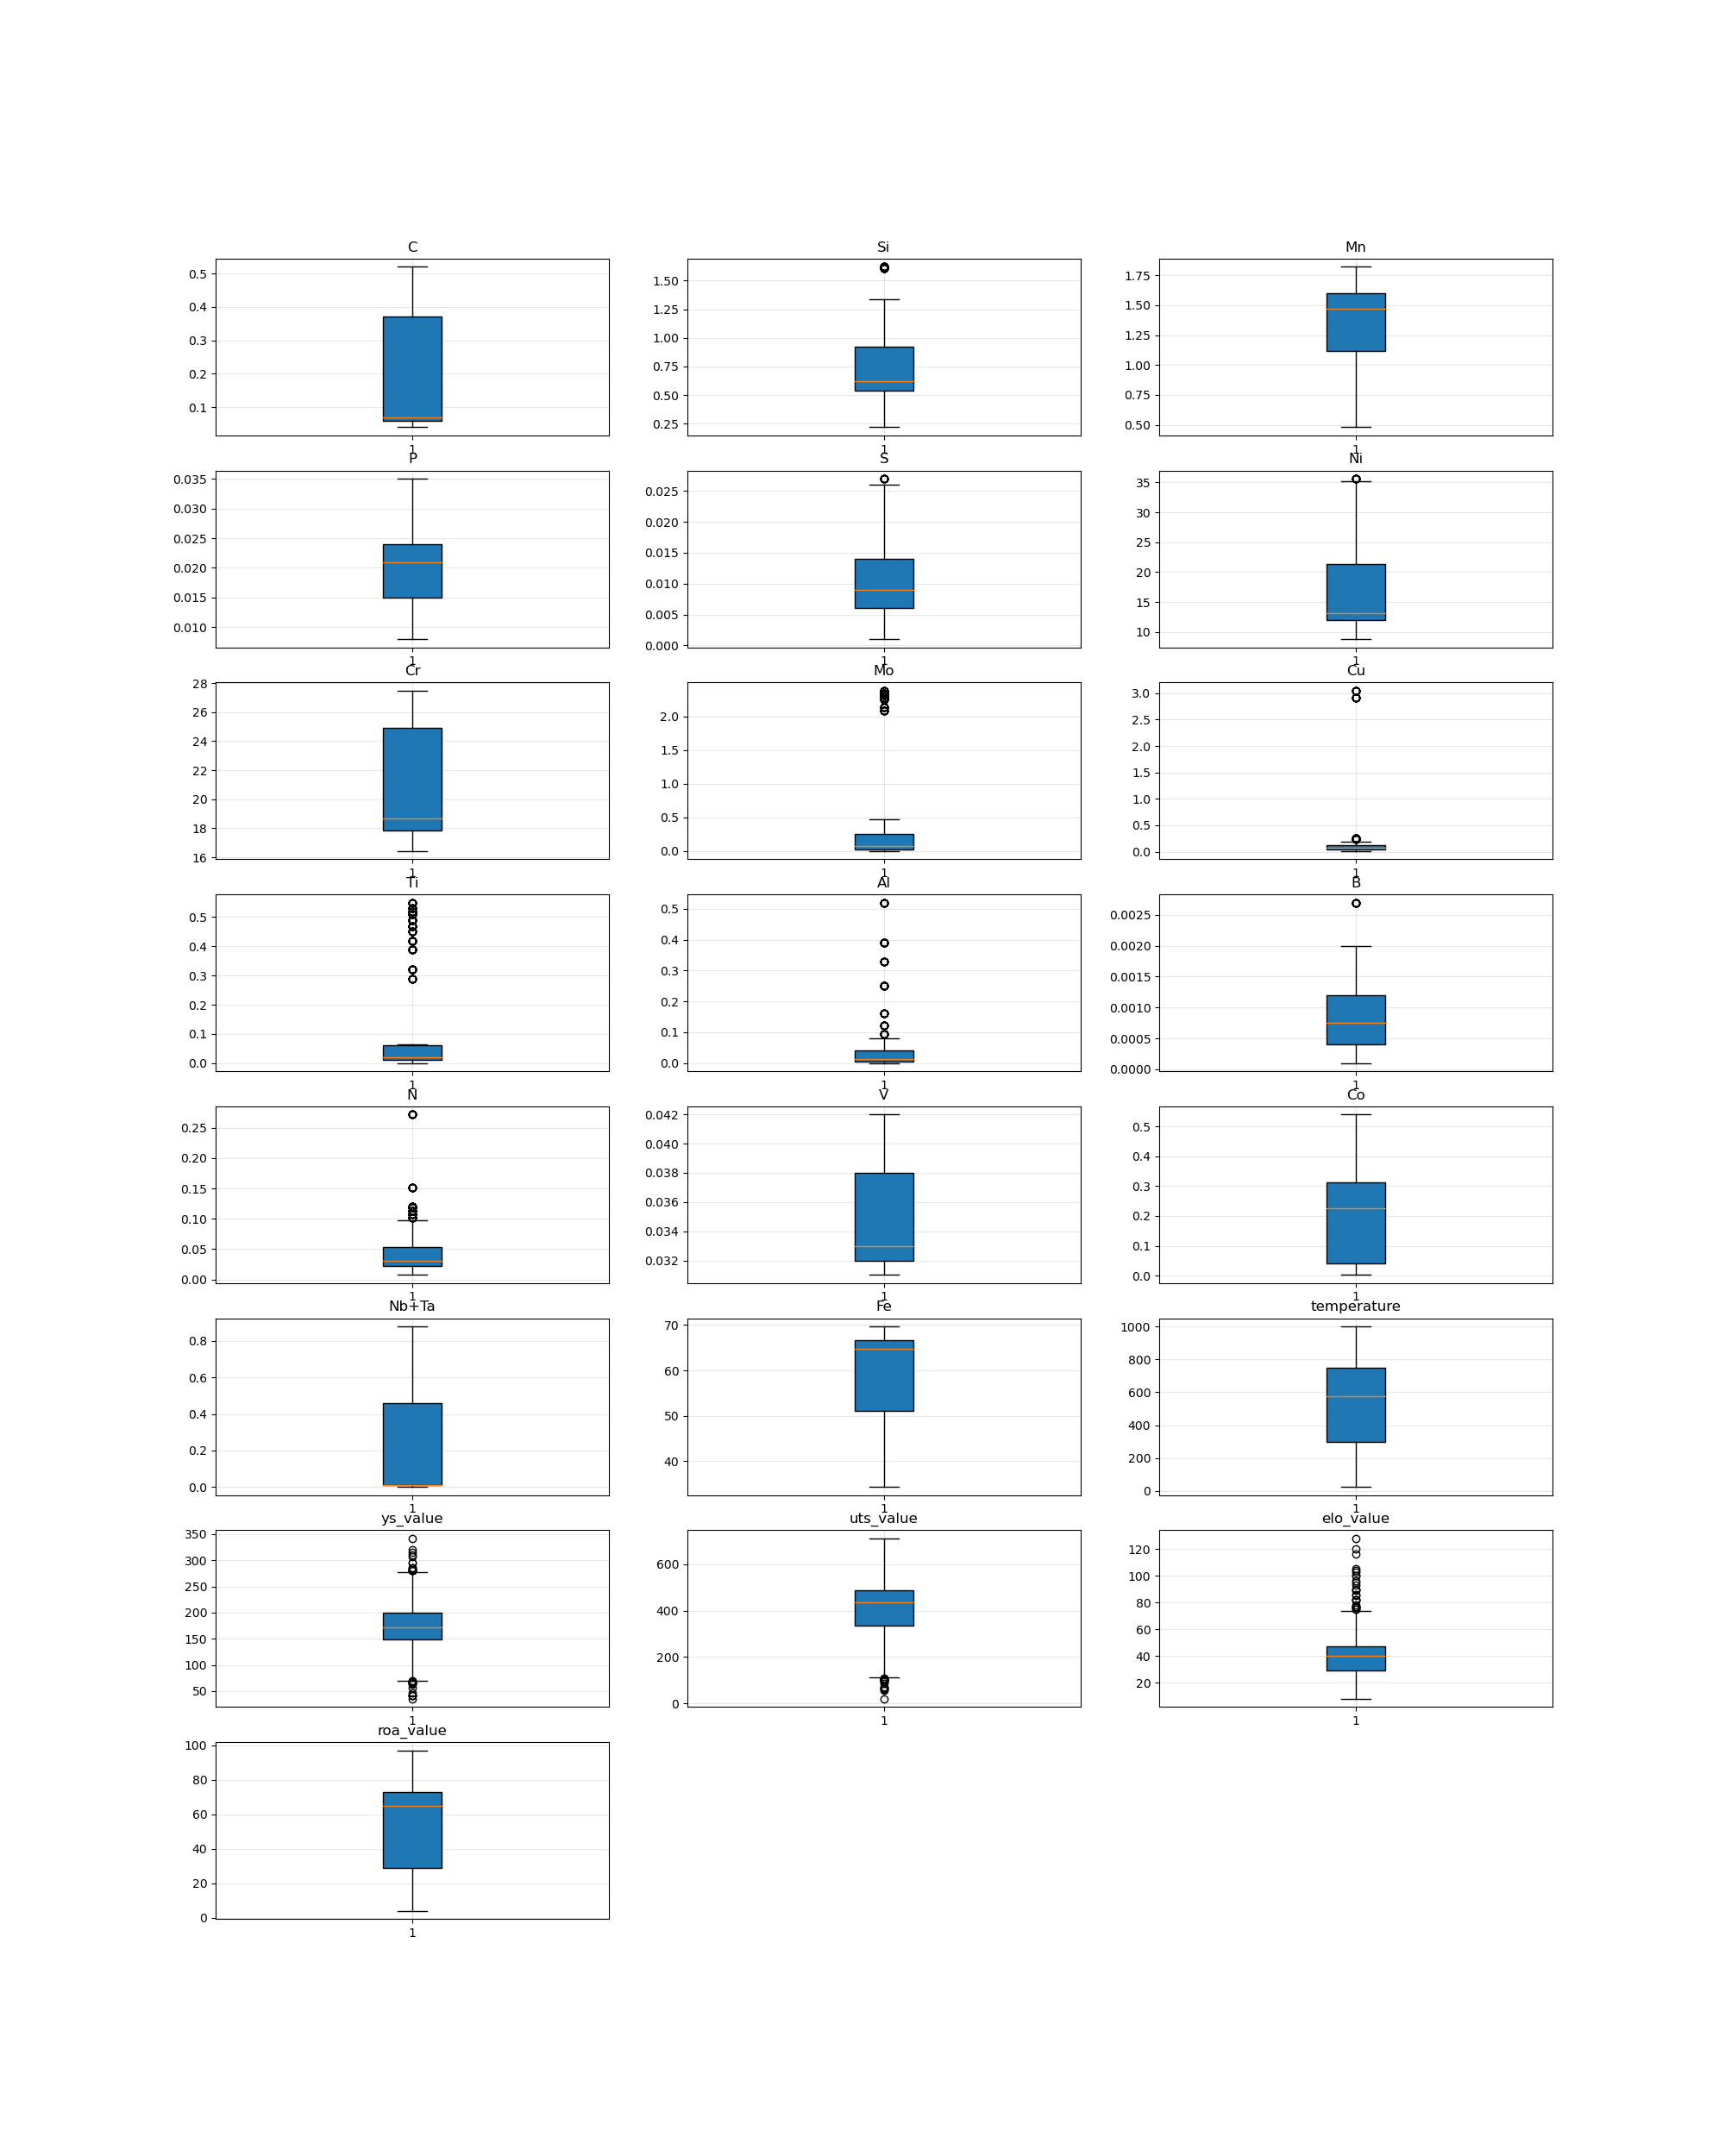
\includegraphics[width=\linewidth]{figures/03_leastsq/statdesc.png}
    \caption{Descriptive statistic of merged\_data.csv}
    \label{fig:enter-label}
\end{figure}

Steel's mechanical properties are influenced by:
\begin{itemize}
    \item \textbf{Chemical composition}: Elements like Carbon (C), Manganese (Mn), and Boron (B) significantly affect strength and ductility
    \item \textbf{Temperature}: Thermal conditions during testing alter material behavior, with higher temperatures generally reducing strength and increasing ductility
    \item \textbf{Microstructure}: Resulting from chemical composition and thermal history
\end{itemize}

The general polynomial approximation of degree $n$ is given by:
\begin{equation}
p_n(x) = \sum_{i=0}^{n} a_i x^i
\end{equation}

For our analysis, we primarily use first-degree polynomial approximation:
\begin{equation}
p_1(x) = a_0 + a_1 x
\end{equation}

This linear model provides a fundamental understanding of the relationship between independent variables (chemical elements and temperature) and dependent variables (mechanical properties).

\subsection{Least Squares Method}

The least squares method minimizes the sum of the squares of the residuals (differences between observed and predicted values). The goal is to find coefficients \( a_0 \) and \( a_1 \) that minimize the residual sum of squares (RSS):
\begin{equation}
RSS = \sum_{i=1}^{n} \left( y_i - (a_0 + a_1 x_i) \right)^2
\end{equation}

The Gram matrix \( G \) is constructed using the inner products of the basis functions. For a first-degree polynomial, the basis functions are \( 1 \) and \( x \). The entries of the Gram matrix are computed as:
\begin{equation}
G_{i,j} = \sum_{k=1}^{n} x_k^{i+j}
\end{equation}


The normal equations for this problem are given by:
\begin{equation}
\begin{bmatrix}
n & \sum_{i=1}^{n} x_i \\
\sum_{i=1}^{n} x_i & \sum_{i=1}^{n} x_i^2
\end{bmatrix}
\begin{bmatrix}
a_0 \\
a_1
\end{bmatrix}
=
\begin{bmatrix}
\sum_{i=1}^{n} y_i \\
\sum_{i=1}^{n} x_i y_i
\end{bmatrix}
\end{equation}

\subsubsection{Algorithm}
\begin{algorithm}[H]
\caption{Least Squares Fit using General Polynomial Approximation}\label{alg:least_squares}
\begin{algorithmic}
\Require Data points $x_i$, $y_i$, degree $n=1$
\Ensure Coefficients $\mathbf{a} = [a_0, a_1]$
\State \textbf{Form the Gram matrix $G$}:
\State $G[0][0] \gets n$
\State $G[0][1] \gets G[1][0] \gets \sum_{i=1}^{n} x_i$
\State $G[1][1] \gets \sum_{i=1}^{n} x_i^2$
\State \textbf{Form the d vector}:
\State $d[0] \gets \sum_{i=1}^{n} y_i$
\State $d[1] \gets \sum_{i=1}^{n} x_i y_i$
\State \textbf{Solve the normal equations}:
\State Solve the linear system $G \cdot \mathbf{a} = d$ for coefficients $\mathbf{a}$
\State \textbf{return} $\mathbf{a}$
\end{algorithmic}
\end{algorithm}

\subsubsection{Python snippet for Least Square}
\begin{lstlisting}[style=custompython][caption={Least Square}, label=code:ls]
import pandas as pd
import numpy as np
import matplotlib.pyplot as plt
import os

# Load data and create directories
df = pd.read_csv('03_leastsq/merged_data.csv')
os.makedirs('03_leastsq/plots', exist_ok=True)
os.makedirs('03_leastsq/results', exist_ok=True)

# Define least squares function
def least_squares_fit(x, y, n):
    G = np.zeros((n+1, n+1))
    b = np.zeros(n+1)
    for j in range(n+1):
        for k in range(n+1):
            G[j, k] = np.sum(x**(j + k))
        b[j] = np.sum(y * x**j)
    try:
        beta = np.linalg.solve(G, b)
    except np.linalg.LinAlgError:
        beta = np.linalg.pinv(G) @ b  # Fallback to pseudo-inverse
    return beta, G, b

# Define variables and y-axis limits
y_cols = ['ys_value', 'uts_value', 'elo_value', 'roa_value']
X_cols = ['C', 'Si', 'Mn', 'P', 'S', 'Ni', 'Cr', 'Mo', 'Cu', 'Ti', 'Al', 'B', 'N', 'V', 'Co', 'Nb+Ta', 'temperature']
ylims_dict = {
    'ys_value': (0, 400),
    'uts_value': (0, 800),
    'elo_value': (0, 120),
    'roa_value': (0, 120)
}

# Initialize results dictionary
beta_results = {}

# Process each variable combination
degrees = [1]
for x_name in X_cols:
    x = df[x_name].values
    for y_name in y_cols:
        y = df[y_name].values
        valid_mask = ~np.isnan(x) & ~np.isnan(y)
        x_valid = x[valid_mask]
        y_valid = y[valid_mask]

        if len(x_valid) == 0:
            continue

        for degree in degrees:
            beta, G, b = least_squares_fit(x_valid, y_valid, degree)
            y_pred = np.polyval(beta[::-1], x_valid)
            l2_norm = np.linalg.norm(y_valid - y_pred)

            # Save coefficients
            if y_name not in beta_results:
                beta_results[y_name] = {}
            beta_results[y_name][x_name] = {
                'beta_0': beta[0] if len(beta) > 0 else None,
                'beta_1': beta[1] if len(beta) > 1 else None
            }

            # Save results to Excel
            with pd.ExcelWriter(f"03_leastsq/results/{x_name}_vs_{y_name}_deg{degree}.xlsx") as writer:
                pd.DataFrame(beta, columns=['Coefficients']).to_excel(writer, sheet_name='Coefficients')
                pd.DataFrame(G).to_excel(writer, sheet_name='Gram_Matrix')
                pd.DataFrame(b, columns=['RHS']).to_excel(writer, sheet_name='RHS')
                pd.DataFrame({'L2_Norm': [l2_norm]}).to_excel(writer, sheet_name='Metrics', index=False)

# Generate bar charts for each dependent variable
for y_name in y_cols:
    if y_name not in beta_results:
        continue

    x_vars = []
    beta1_values = []
    for x_name in X_cols:
        if x_name in beta_results[y_name]:
            x_vars.append(x_name)
            beta1 = beta_results[y_name][x_name]['beta_1']
            beta1_values.append(beta1 if beta1 is not None else 0)

    plt.figure(figsize=(12, 6))
    plt.bar(x_vars, beta1_values, color='blue')
    plt.xlabel('Independent Variables')
    plt.ylabel('Beta_1 Coefficient')
    plt.yscale('symlog')
    plt.title(f'Beta_1 Coefficients for {y_name}')
    plt.xticks(rotation=45, ha='right')
    plt.grid(axis='y', linestyle='--', alpha=0.7)
    plt.tight_layout()
    plt.savefig(f'03_leastsq/plots/bar_charts/{y_name}_beta1_bar_chart.png')
    plt.close()

# Save beta coefficients to Excel
beta_df = pd.DataFrame(beta_results).T
beta_df.to_excel("03_leastsq/results/beta_coefficients.xlsx")

print("Beta coefficients collected and saved.")
\end{lstlisting}

\newpage
\subsection{Results}
Our analysis reveals several important relationships:
\subsubsection{Example 1: Temperature vs Yield Strength}
\begin{itemize}
    \item \textbf{Gram matrix}:
    \[
    G = \begin{bmatrix}
    773 & 364,875 \\
    364,875 & 228,744,375
    \end{bmatrix}
    \]
    \item \textbf{d vector}:
    \[
    d = \begin{bmatrix}
    135,174 \\
    55,810,200
    \end{bmatrix}
    \]
    \item \textbf{Coefficients}:
    \[
    \mathbf{a} = \begin{bmatrix}
    241.65 \\
    -0.14
    \end{bmatrix}
    \]
\end{itemize}

The negative coefficient for temperature indicates that yield strength decreases with increasing temperature, which aligns with expected material behavior as higher temperatures reduce material strength.

\begin{figure}[H]
    \centering
    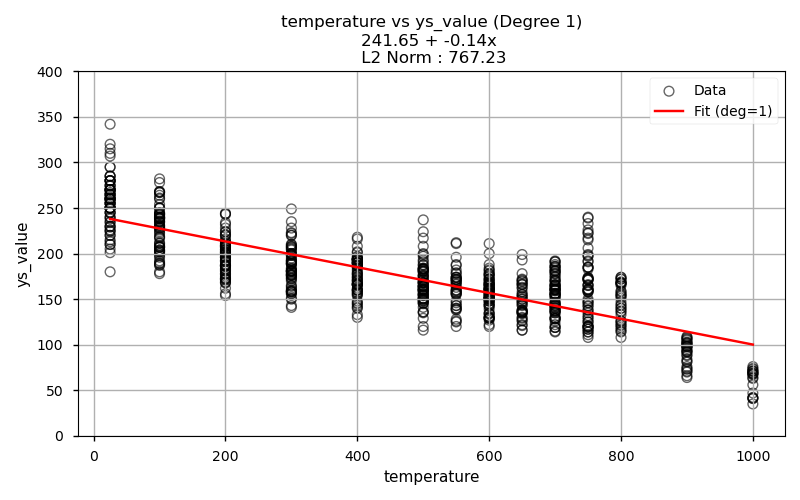
\includegraphics[width=\imagewidthone\textwidth]{figures/03_leastsq/temperature_vs_ys_value_deg1.png}
    \caption{Relationship between temperature (in Kelvin) and Yield Strength (in MPa)}
\end{figure}


\newpage
\subsubsection{Example 2: Boron vs Yield Strength}
\begin{itemize}
    \item \textbf{Gram matrix}:
    \[
    G = \begin{bmatrix}
    565 & 0.48 \\
    0.48 & 0.00
    \end{bmatrix}
    \]
    \item \textbf{d vector}:
    \[
    d = \begin{bmatrix}
    99,733 \\
    86.47
    \end{bmatrix}
    \]
    \item \textbf{Coefficients}:
    \[
    \mathbf{a} = \begin{bmatrix}
    171.24 \\
    6,176.45
    \end{bmatrix}
    \]
\end{itemize}

Boron shows a strong positive correlation with yield strength, demonstrating its effectiveness as a microalloying element in enhancing steel strength.

\begin{figure}[H]
    \centering
    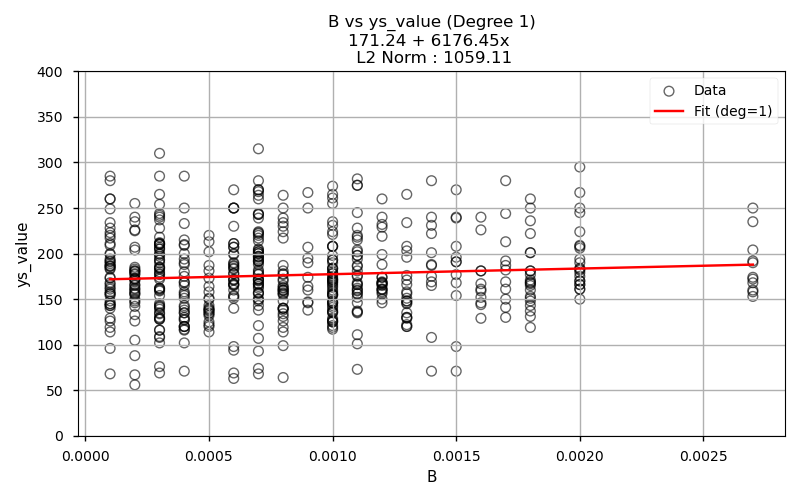
\includegraphics[width=\imagewidthone\textwidth]{figures/03_leastsq/B_vs_ys_value_deg1.png}
    \caption{Relationship between Boron (wt\%) and Yield Strength (in MPa)}
\end{figure}


\newpage
\subsubsection{Example 3: Carbon vs Reduction of Area}
\begin{itemize}
    \item \textbf{Gram matrix}:
    \[
    G = \begin{bmatrix}
    773 & 138.07 \\
    138.07 & 45.09
    \end{bmatrix}
    \]
    \item \textbf{d vector}:
    \[
    d = \begin{bmatrix}
    42,137 \\
    5,132.12
    \end{bmatrix}
    \]
    \item \textbf{Coefficients}:
    \[
    \mathbf{a} = \begin{bmatrix}
    75.45 \\
    -117.23
    \end{bmatrix}
    \]
\end{itemize}

Carbon content exhibits a negative relationship with reduction of area, indicating that higher carbon levels reduce ductility.

\begin{figure}[H]
    \centering
    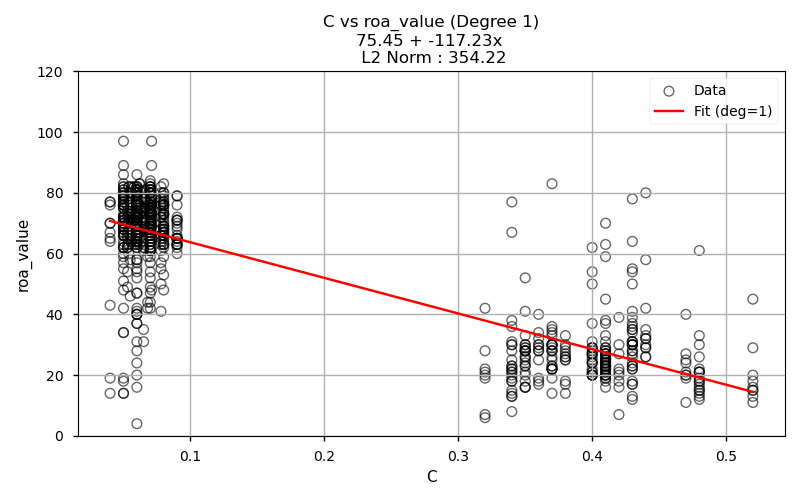
\includegraphics[width=\imagewidthone\textwidth]{figures/03_leastsq/C_vs_roa_value_deg1.png}
    \caption{Relationship between Carbon (wt\%) and Reduction of Area (in \%)}
\end{figure}

\newpage
\subsubsection{Example 4: Silicon vs Elongation}
\begin{itemize}
    \item \textbf{Gram matrix}:
    \[
    G = \begin{bmatrix}
    773 & 562.02 \\
    562.02 & 473.82
    \end{bmatrix}
    \]
    \item \textbf{d vector}:
    \[
    d = \begin{bmatrix}
    31,188 \\
    20,852.98
    \end{bmatrix}
    \]
    \item \textbf{Coefficients}:
    \[
    \mathbf{a} = \begin{bmatrix}
    60.67 \\
    -27.96
    \end{bmatrix}
    \]
\end{itemize}

Silicon also shows a negative relationship with elongation, suggesting that increased silicon content reduces steel ductility.

\begin{figure}[H]
    \centering
    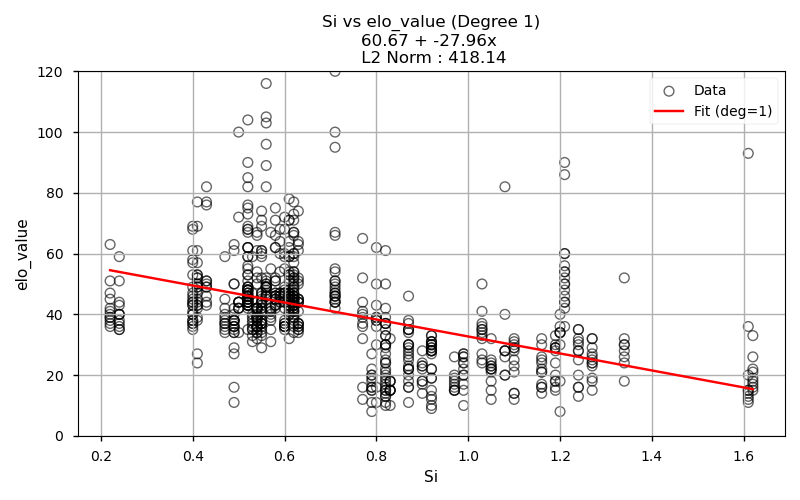
\includegraphics[width=\imagewidthone\textwidth]{figures/03_leastsq/Si_vs_elo_value_deg1.png}
    \caption{Relationship between Silicon (wt\%) and Elongation (in \%)}
\end{figure}

The following bar charts illustrate the beta coefficients for each independent variable across different mechanical properties:



\begin{figure}[H]
    \centering
    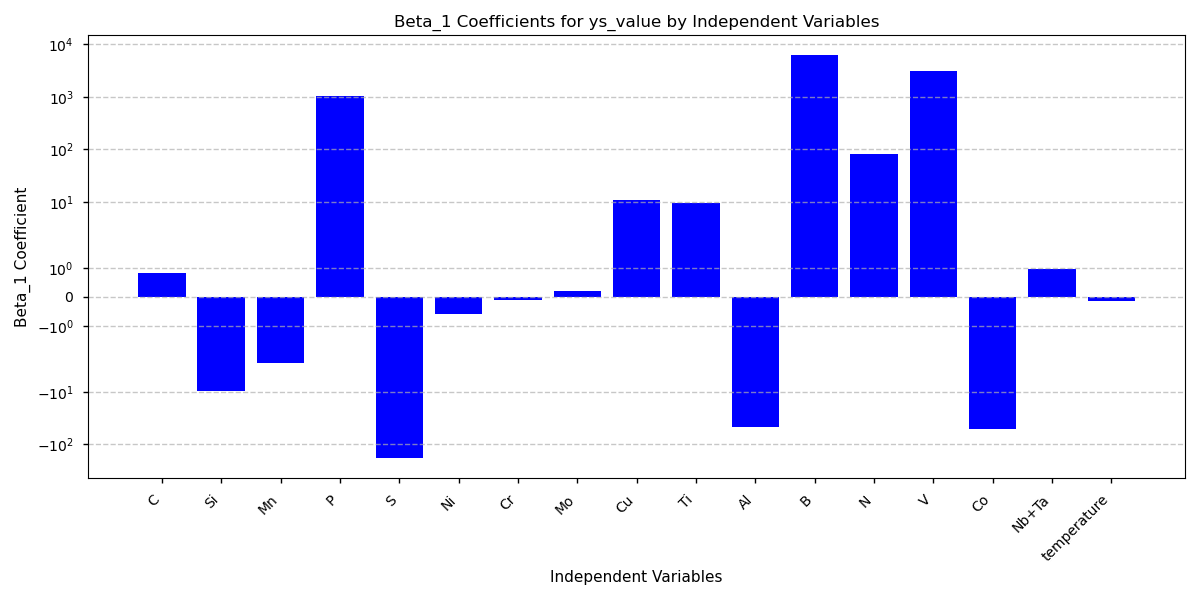
\includegraphics[width=\imagewidth\textwidth]{figures/03_leastsq/ys_value_beta1_bar_chart.png}
    \caption{Relationship between independent variables and Yield Strength (in MPa)}
\end{figure}
\begin{figure}[H]
    \centering
    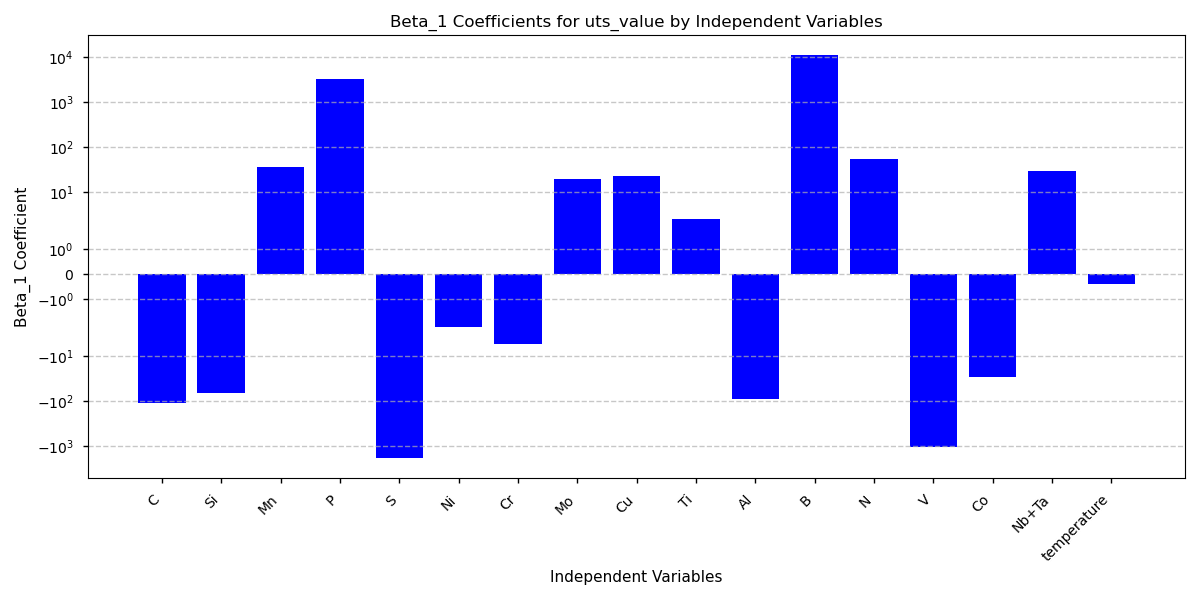
\includegraphics[width=\imagewidth\textwidth]{figures/03_leastsq/uts_value_beta1_bar_chart.png}
    \caption{Relationship between independent variables and Ultimate Tensile Strength (in MPA)}
\end{figure}
\begin{figure}[H]
    \centering
    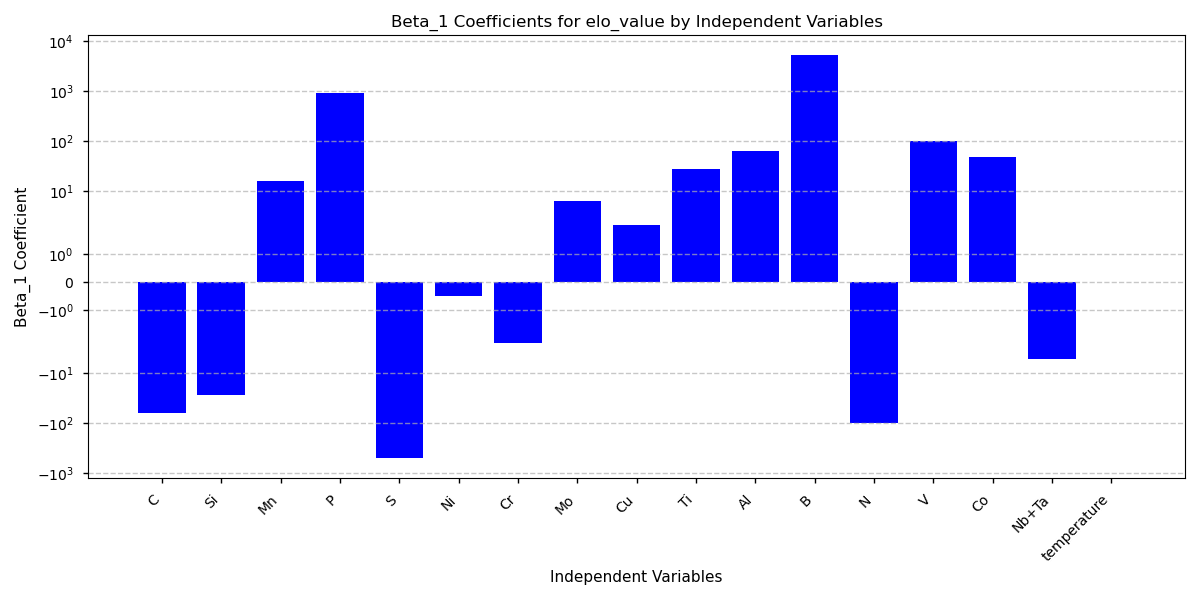
\includegraphics[width=\imagewidth\textwidth]{figures/03_leastsq/elo_value_beta1_bar_chart.png}
    \caption{Relationship between independent variables and \%Elongation}
\end{figure}
\begin{figure}[H]
    \centering
    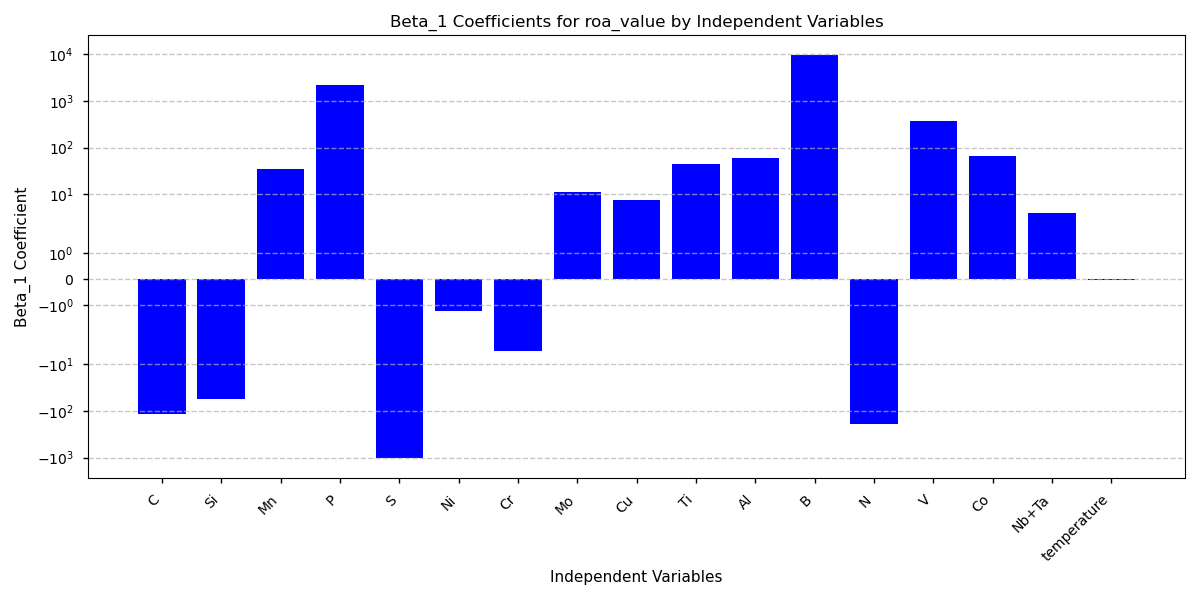
\includegraphics[width=\imagewidth\textwidth]{figures/03_leastsq/roa_value_beta1_bar_chart.png}
    \caption{Relationship between independent variables and \%Reduction of Area}
\end{figure}

\newpage
\subsection{Key Observations}
\begin{itemize}
    \item The Gram matrix $G$ is symmetric and positive definite, ensuring a unique solution for the normal equations.
    \item The coefficients $\mathbf{a}$ provide the best linear approximation for the relationship between variables.
    \item The signs of $a_1$ indicate the direction of the relationship between independent variables and mechanical properties:
    \begin{itemize}
        \item Positive coefficients: Strengthening elements (e.g., Boron for YS)
        \item Negative coefficients: Ductility-reducing elements (e.g., Carbon for RA)
    \end{itemize}
    \item Elements like Carbon and Silicon generally reduce ductility while increasing strength, demonstrating the typical strength-ductility trade-off in steels.
    \item Boron shows exceptional effectiveness in increasing yield strength despite its low concentration.
    \item \textbf{Important Note:} While we observe correlations between variables, it is crucial to remember that correlation does not imply causation. These relationships should be validated through further experimental and mechanistic studies before drawing definitive conclusions about causal relationships.
\end{itemize}

This least squares analysis provides valuable insights into how chemical composition and temperature affect steel's mechanical properties. The results can guide steel selection and alloy design by quantifying the impact of specific elements and testing conditions. Further analysis using higher-degree polynomials or multivariate models could provide more comprehensive understanding of these relationships.



\section{Integration}
\subsection{Real Case: Calculation of Enthalpy}
The calculation of sensible heat for materials like calcium oxide (CaO) involves evaluating integrals of thermodynamic functions. The enthalpy change of CaO over a temperature range can be expressed as:

\begin{equation}
\Delta H = \int_{T_1}^{T_2} C_p(T) dT
\end{equation}

Where \(C_p(T)\) is the temperature-dependent specific heat capacity. Due to the complexity of \(C_p(T)\) functions, analytical integration is often impractical, necessitating numerical approximation methods.

For example, the heat capacity of CaO is modeled by:
\begin{equation}
C_p(T) = 57.753 + (-10.779)\times10^{-3}T + (-11.51)\times10^{5}T^{-2} + 5.328\times10^{-6}T^2
\end{equation}

\subsection{Method}
\subsubsection{Left Rectangular Method}
This method approximates the integral using rectangles built on left endpoints. The formula is:

\begin{equation}
\int_{a}^{b} f(x)dx \approx h\sum_{i=0}^{n-1} f(a + i\cdot h)
\end{equation}

\begin{algorithm}[H]
\caption{Left Rectangular Integration}
\begin{algorithmic}[1]
\Require Function $f$, interval $[a, b]$, number of subintervals $n$
\Ensure Approximation of $\int_{a}^{b} f(x) dx$
\State $h \gets \frac{b - a}{n}$
\State $S \gets 0$
\For{$i = 0$ to $n-1$}
    \State $S \gets S + f(a + i \cdot h) \cdot h$
\EndFor
\State \textbf{return} $S$
\end{algorithmic}
\end{algorithm}

Python snippet for the left rectangle method:
\begin{lstlisting}[style=custompython][caption={Left rectangle integration method}, label=code:lr integra]
def left_rectangular(f, a, b, n):
    h = (b - a)/n
    x = np.linspace(a, b, n+1)[:-1]
    return h * np.sum(f(x))
\end{lstlisting}


This method provides a lower bound approximation for monotonically increasing functions.


\subsubsection{Right Rectangular Method}
The right endpoint variant calculates:

\begin{equation}
\int_{a}^{b} f(x)dx \approx h\sum_{i=1}^{n} f(a + i\cdot h)
\end{equation}

\begin{algorithm}[H]
\caption{Right Rectangular Integration}
\begin{algorithmic}[1]
\Require Function $f$, interval $[a, b]$, number of subintervals $n$
\Ensure Approximation of $\int_{a}^{b} f(x) dx$
\State $h \gets \frac{b - a}{n}$
\State $S \gets 0$
\For{$i = 1$ to $n$}
    \State $S \gets S + f(a + i \cdot h) \cdot h$
\EndFor
\State \textbf{return} $S$
\end{algorithmic}
\end{algorithm}

Python snippet for the right rectangle method:
\begin{lstlisting}[style=custompython][caption={Right rectangle integration method}, label=code:rr integra]
def right_rectangular(f, a, b, n):
    h = (b - a)/n
    x = np.linspace(a, b, n+1)[1:]
    return h * np.sum(f(x))
\end{lstlisting}

Gives an upper bound for increasing functions and vice versa for decreasing functions.

\subsubsection{Trapezoid Method}

This method averages the left and right estimates using trapezoids:

\begin{equation}
\int_{a}^{b} f(x)dx \approx \frac{h}{2}\left[f(a) + 2\sum_{i=1}^{n-1}f(a+i\cdot h) + f(b)\right]
\end{equation}


\begin{algorithm}[H]
\caption{Trapezoid Integration}
\begin{algorithmic}[1]
\Require Function $f$, interval $[a, b]$, number of subintervals $n$
\Ensure Approximation of $\int_{a}^{b} f(x) dx$
\State $h \gets \frac{b - a}{n}$
\State $S \gets \frac{h}{2} \cdot (f(a) + f(b))$
\For{$i = 1$ to $n-1$}
    \State $S \gets S + h \cdot f(a + i \cdot h)$
\EndFor
\State \textbf{return} $S$
\end{algorithmic}
\end{algorithm}

Python snippet for the trapezoidal method:
\begin{lstlisting}[style=custompython][caption={Trapezoidal integration method}, label=code:tra integra]
def composite_trapezoid(f, a, b, n):
    h = (b - a)/n
    x = np.linspace(a, b, n+1)
    y = f(x)
    return h/2 * (y[0] + 2*np.sum(y[1:-1]) + y[-1])
\end{lstlisting}


Achieves second-order convergence through its linear approximation.


\subsubsection{Newton-Cotes Method}

The general Newton-Cotes formula for degree \(k\) is:

\begin{equation}
\int_{a}^{b} f(x)dx \approx \frac{h}{k!}\sum_{i=0}^{k} w_i f(a + i\cdot h)
\end{equation}
Where \(w_i\) are coefficients derived from polynomial interpolation.
For Simpson's rule (degree 2):
\begin{equation}
\int_{a}^{b} f(x)dx \approx \frac{h}{3}\left[f(a) + 4f\left(\frac{a+b}{2}\right) + f(b)\right]
\end{equation}


\begin{algorithm}[H]
\caption{Newton-Cotes Integration}
\begin{algorithmic}[1]
\Require Function $f$, interval $[a, b]$, number of subintervals $n$
\Ensure Approximation of $\int_{a}^{b} f(x) dx$
\State $h \gets \frac{b - a}{n}$
\State $S \gets 0$
\For{$i = 0$ to $n-1$}
    \State $x_i \gets a + i \cdot h$
    \State $S \gets S + f(x_i)$
\EndFor
\State \textbf{Calculate divided differences}
\For{$k = 2$ to $n$}
    \State $d_k \gets 0$
    \For{$i = 0$ to $n-k$}
        \State $d_k \gets d_k + \binom{n-i-1}{k-1} \cdot f(x_i + (k-1) \cdot h)$
    \EndFor
    \State $S \gets S + \frac{h}{k!} \cdot d_k$
\EndFor
\State \textbf{return} $S$
\end{algorithmic}
\end{algorithm}

Python snippet for the Newton-cotes method:
\begin{lstlisting}[style=custompython][caption={Newton-cotes integration method}, label=code:nc integra]
def newton_cotes(f, a, b, n, degree):
    if degree not in [2, 3, 4]:
        raise ValueError
    
    num_sub = n // degree
    if num_sub < 1:
        num_sub = 1
    actual_n = num_sub * degree
    
    h = (b - a) / actual_n
    total = 0.0
    
    for i in range(num_sub):
        sub_a = a + i * degree * h
        sub_b = sub_a + degree * h
        x = np.linspace(sub_a, sub_b, degree + 1)
        y = f(x)
        
        if degree == 2:
            total += h/3 * (y[0] + 4*y[1] + y[2])
        elif degree == 3: 
            total += 3*h/8 * (y[0] + 3*y[1] + 3*y[2] + y[3])
        elif degree == 4: 
            total += 2*h/45 * (7*y[0] + 32*y[1] + 12*y[2] + 32*y[3] + 7*y[4])
    
    return total
\end{lstlisting}

\subsubsection{Romberg Integration}
This method combines Richardson extrapolation with trapezoidal estimates:
\begin{equation}
R_{k,j} = \frac{4^j R_{k,j-1} - R_{k-1,j-1}}{4^j - 1}
\end{equation}

\begin{algorithm}[H]
\caption{Romberg Integration}
\begin{algorithmic}[1]
\Require Function $f$, interval $[a, b]$, maximum number of extrapolations $K$
\Ensure Approximation of $\int_{a}^{b} f(x) dx$
\State Initialize $T[K+1]$ with $T[0] = \frac{h}{2} (f(a) + f(b))$
\For{$k = 1$ to $K$}
    \State $h \gets \frac{h}{2}$
    \State $T[k] \gets T[k-1]/2 + h \sum_{i=0}^{2^{k-1}} f(a + (2i + 1)h)$
    \For{$j = 1$ to $k$}
        \State $T[k] \gets (4^{j}T[k] - T[k-1])/(4^{j} - 1)$
    \EndFor
\EndFor
\State \textbf{return} $T[K]$
\end{algorithmic}
\end{algorithm}
Python snippet for the Romberg method:
\begin{lstlisting}[style=custompython][caption={Romberg integration method}, label=code:ro integra]
def romberg(f, a, b, max_k):
    T = np.zeros(max_k + 1)
    h = b - a
    T[0] = (h / 2) * (f(a) + f(b))
    
    for k in range(1, max_k + 1):
        h /= 2
        x_new = a + h * np.arange(1, 2**k, 2)
        T[k] = T[k-1]/2 + h * np.sum(f(x_new))
    
    for j in range(1, max_k + 1):
        for k in range(j, max_k + 1):
            T[k] = (4**j * T[k] - T[k-1]) / (4**j - 1)
    
    return T[max_k]
\end{lstlisting}

\subsubsection{Gauss-Legendre Integration}

Uses optimally spaced points and weights:
\begin{equation}
\int_{a}^{b} f(x)dx \approx \frac{b-a}{2}\sum_{i=1}^{n} w_i f\left(\frac{b-a}{2}x_i + \frac{a+b}{2}\right)
\end{equation}

\begin{algorithm}[H]
\caption{Gauss-Legendre Integration}
\begin{algorithmic}[1]
\Require Function $f$, interval $[a, b]$, number of points $n$
\Ensure Approximation of $\int_{a}^{b} f(x) dx$
\State Compute Legendre polynomials $P_n(x)$
\State Compute roots $x_i$ and weights $w_i$ for $P_n(x)$
\State Transform roots and weights to interval $[a, b]$
\State $S \gets 0$
\For{$i = 0$ to $n-1$}
    \State $S \gets S + w_i \cdot f(x_i)$
\EndFor
\State \textbf{return} $S \cdot \frac{b-a}{2}$
\end{algorithmic}
\end{algorithm}

Python snippet for the Gauss-Legendre method:
\begin{lstlisting}[style=custompython][caption={Gauss-Legendre integration method}, label=code:gl integra]
def legendre_poly(n, x):
    if n == 0:
        return np.ones_like(x)
    elif n == 1:
        return x
    else:
        return ((2*n-1)*x*legendre_poly(n-1,x) - (n-1)*legendre_poly(n-2,x))/n

def legendre_roots_weights(n):
    roots = np.zeros(n)
    weights = np.zeros(n)
    x0 = np.cos(np.pi * (np.arange(1, n+1) - 0.25) / (n + 0.5))
    
    for i in range(n):
        x = x0[i]
        while True:
            P, dP = legendre_poly(n, x), 0
            # Calculate derivative using recurrence
            if x != 0:
                dP = n*(legendre_poly(n-1,x) - x*legendre_poly(n,x))/(1-x**2)
            else:
                dP = n*legendre_poly(n-1,x)
            
            dx = P/dP
            x -= dx
        
        roots[i] = x
        weights[i] = 2/((1-x**2)*dP**2)
    
    return roots, weights

def gauss_legendre(f, a, b, n):
    x, w = legendre_roots_weights(n)
    x_trans = 0.5*(b-a)*x + 0.5*(b+a)
    w_trans = 0.5*(b-a)*w
    return np.sum(w_trans * f(x_trans))
    
\end{lstlisting}


\subsubsection{Gauss-Chebyshev Integration}

Employs weighted integration with Chebyshev polynomials:
\begin{equation}
\int_{a}^{b} f(x)dx \approx \frac{\pi}{n}\sum_{k=1}^{n} f\left(\frac{a+b}{2} + \frac{b-a}{2}\cos\left(\frac{2k-1}{2n}\pi\right)\right)
\end{equation}


\begin{algorithm}[H]
\caption{Gauss-Chebyshev Integration}
\begin{algorithmic}[1]
\Require Function $f$, interval $[a, b]$, number of points $n$
\Ensure Approximation of $\int_{a}^{b} f(x) dx$
\State Compute Chebyshev polynomials $T_n(x)$
\State Compute roots $x_i$ and weights $w_i$ for $T_n(x)$
\State Transform roots and weights to interval $[a, b]$
\State $S \gets 0$
\For{$i = 0$ to $n-1$}
    \State $S \gets S + w_i \cdot f(x_i)$
\EndFor
\State \textbf{return} $S \cdot \frac{b-a}{2}$
\end{algorithmic}
\end{algorithm}

Python snippet for the Gauss-Chebyshev method:
\begin{lstlisting}[style=custompython][caption={Gauss-Chebyshev integration method}, label=code:gc integra]
def chebyshev_poly(n):
    if n == 0:
        return [1]
    elif n == 1:
        return [1, 0]
    else:
        coeff = 2*np.pad(chebyshev_poly(n-1), (0,1), 'constant')
        coeff[:-2] -= chebyshev_poly(n-2)
        return coeff

def chebyshev_roots(n):
    return np.cos(np.pi * (2*np.arange(1, n+1) - 1) / (2*n))

def chebyshev_weights(n):
    return np.full(n, np.pi/n)

def gauss_chebyshev(f, a, b, n):
    roots = chebyshev_roots(n)
    weights = chebyshev_weights(n)
    
    # Transform from [-1,1] to [a,b]
    x_trans = 0.5*(b - a)*roots + 0.5*(b + a)
    w_trans = 0.5*(b - a)*weights
    
    # Account for the weight function
    return np.sum(w_trans * f(x_trans) * np.sqrt(1 - ((2*x_trans-(b+a))/(b-a))**2))
    
\end{lstlisting}


% \subsubsection*{Key Observations}
% \begin{itemize}
%     \item Left and Right Rectangular methods are simple but less accurate.
%     \item Trapezoid method provides better accuracy by considering function values at both ends of each subinterval.
%     \item Newton-Cotes method uses polynomial interpolation for higher accuracy.
%     \item Romberg method improves accuracy by extrapolation.
%     \item Gauss-Legendre and Gauss-Chebyshev methods use optimal points and weights for high accuracy.
% \end{itemize}

% \begin{lstlisting}
% def left_rectangular(f, a, b, n):
%     h = (b - a)/n
%     x = np.linspace(a, b, n+1)[:-1]
%     return h * np.sum(f(x))

% def right_rectangular(f, a, b, n):
%     h = (b - a)/n
%     x = np.linspace(a, b, n+1)[1:]
%     return h * np.sum(f(x))
% \end{lstlisting}
\subsection{Python snippet for Integration comparison}

\begin{lstlisting}[style=custompython][caption={Comparison for various integration method}, label=code:comparison integra]
import numpy as np
import pandas as pd
import matplotlib.pyplot as plt
import os

# Define various integration methods
def left_rectangular(f, a, b, n):
    h = (b - a)/n
    x = np.linspace(a, b, n+1)[:-1]
    return h * np.sum(f(x))

def right_rectangular(f, a, b, n):
    h = (b - a)/n
    x = np.linspace(a, b, n+1)[1:]
    return h * np.sum(f(x))

def composite_trapezoid(f, a, b, n):
    h = (b - a)/n
    x = np.linspace(a, b, n+1)
    y = f(x)
    return h/2 * (y[0] + 2*np.sum(y[1:-1]) + y[-1])

def newton_cotes(f, a, b, n, degree=2):
    if degree not in [2, 3, 4]:
        raise ValueError
    
    num_sub = n // degree
    actual_n = num_sub * degree
    
    h = (b - a) / actual_n
    total = 0.0
    
    for i in range(num_sub):
        sub_a = a + i * degree * h
        sub_b = sub_a + degree * h
        x = np.linspace(sub_a, sub_b, degree + 1)
        y = f(x)
        
        if degree == 2:
            total += h/3 * (y[0] + 4*y[1] + y[2])
        elif degree == 3: 
            total += 3*h/8 * (y[0] + 3*y[1] + 3*y[2] + y[3])
        elif degree == 4: 
            total += 2*h/45 * (7*y[0] + 32*y[1] + 12*y[2] + 32*y[3] + 7*y[4])
    
    return total

def romberg(f, a, b, max_k):
    T = np.zeros(max_k + 1)
    h = b - a
    T[0] = (h / 2) * (f(a) + f(b))
    
    for k in range(1, max_k + 1):
        h /= 2
        x_new = a + h * np.arange(1, 2**k, 2)
        T[k] = T[k-1]/2 + h * np.sum(f(x_new))
    
    for j in range(1, max_k + 1):
        for k in range(j, max_k + 1):
            T[k] = (4**j * T[k] - T[k-1]) / (4**j - 1)
    
    return T[max_k]

def gauss_legendre(f, a, b, n):
    x, w = legendre_roots_weights(n)
    x_trans = 0.5*(b-a)*x + 0.5*(b+a)
    w_trans = 0.5*(b-a)*w
    return np.sum(w_trans * f(x_trans))

def gauss_chebyshev(f, a, b, n):
    roots = chebyshev_roots(n)
    weights = chebyshev_weights(n)
    
    x_trans = 0.5*(b - a)*roots + 0.5*(b + a)
    w_trans = 0.5*(b - a)*weights
    
    return np.sum(w_trans * f(x_trans) * np.sqrt(1 - ((2*x_trans-(b+a))/(b-a))**2))

# Generate results for different methods
def generate_results(f, a, b, ns):
    methods = [
        ('Left Rect', left_rectangular),
        ('Right Rect', right_rectangular),
        ('Trapezoid', composite_trapezoid),
        ('Newton-Cotes 2', lambda f, a, b, n: newton_cotes(f, a, b, n, 2)),
        ('Newton-Cotes 3', lambda f, a, b, n: newton_cotes(f, a, b, n, 3)),
        ('Newton-Cotes 4', lambda f, a, b, n: newton_cotes(f, a, b, n, 4)),
        ('Romberg', lambda f, a, b, n: romberg(f, a, b, n)),
        ('Gauss-Legendre', gauss_legendre),
        ('Gauss-Chebyshev', gauss_chebyshev)
    ]
    
    exact = exact_integral(a, b)
    
    data = []
    for n in ns:
        row = {'n': n}
        for name, method in methods:
            try:
                row[name] = method(f, a, b, n)
            except Exception as e:
                row[name] = np.nan
        data.append(row)
    
    results_df = pd.DataFrame(data)
    results_df['Exact'] = exact
    
    # Create error DataFrame
    error_data = {'n': ns}
    for name, _ in methods:
        error_data[name + '_error'] = np.abs((results_df[name] - exact)/exact)
    
    error_df = pd.DataFrame(error_data)
    error_df = error_df.rename(columns={c: c.replace('_error', '') for c in error_df.columns if c != 'n'})
    
    return results_df, error_df

# Example function and exact integral
def original_function(x):
    return 57.753 + (-10.779)*1e-3*x + (-11.51)*1e5/(x**2) + 5.328*1e-6*x**2

def exact_integral(a, b):
    def integral(x):
        return 57.753*x + (-10.779)*1e-3*(x**2)/2 + (-11.51)*1e5*(-1/x) + 5.328*1e-6*(x**3)/3
    return integral(b) - integral(a)

if __name__ == "__main__":
    a = 298
    b = 1500
    ns = np.arange(1, 21)
    
    results_df, error_df = generate_results(original_function, a, b, ns)
    
    # Plot results
    plt.figure(figsize=(10, 6))
    for col in results_df.columns:
        if col not in ['n', 'Exact']:
            plt.plot(results_df['n'], results_df[col], label=col)
    plt.plot(results_df['n'], results_df['Exact'], 'k--', label='Exact')
    plt.xlabel('n')
    plt.ylabel('Integral Value')
    plt.title('Integration Method Comparison')
    plt.legend()
    plt.grid(True)
    plt.show()

    plt.figure(figsize=(10, 6))
    for col in error_df.columns:
        if col != 'n':
            plt.plot(error_df['n'], error_df[col], label=col)
    plt.xlabel('n')
    plt.ylabel('Absolute Error')
    plt.yscale("log")
    plt.title('Integration Error Comparison')
    plt.legend()
    plt.grid(True)
    plt.show()

\end{lstlisting}

\subsection{Results}

The convergence behavior across methods is shown in Table \ref{tab:integration_results}. Figure \ref{fig:integration_results} demonstrates the approximation quality for different \(n\), while Figure \ref{fig:integration_errors} presents the error characteristics.

\begin{landscape}
% \begin{table}[H]
\begin{table}[htbp]
\centering
\caption{Integration Results}
\label{tab:integration_results}
\begin{tabular}{lrrrrrrrrrrrrrrrrrrrr}
\toprule
$n$ & \multicolumn{1}{c}{Left Rect} & \multicolumn{1}{c}{Right Rect} & \multicolumn{1}{c}{Trapezoid} & \multicolumn{1}{c}{NC 2} & NC 3 & NC 4 & Romberg & Legendre & Chebyshev & Exact \\
\midrule
1 & 50,547.56 & 63,779.26 & 57,163.41 & 59,878.09 & 60,201.93 & 60,515.38 & 59,878.09 & 61,235.44 & 96,188.40 & 60,623.26 \\
2 & 25,891.50 & 62,507.35 & 59,199.42 & 59,878.09 & 60,201.93 & 60,515.38 & 60,274.08 & 61,002.63 & 67,343.82 & 60,623.26 \\
3 & 57,659.03 & 62,069.60 & 59,864.32 & 59,878.09 & 60,201.93 & 60,515.38 & 60,598.10 & 60,705.79 & 63,222.57 & 60,623.26 \\
4 & 58,502.56 & 61,810.48 & 60,156.52 & 60,475.55 & 60,201.93 & 60,515.38 & 60,594.59 & 60,639.30 & 62,060.86 & 60,623.26 \\
5 & 58,985.91 & 61,632.25 & 60,309.08 & 60,475.55 & 60,201.93 & 60,515.38 & 60,623.72 & 60,626.19 & 61,549.60 & 60,623.26 \\
6 & 59,295.52 & 61,500.80 & 60,398.16 & 60,576.11 & 60,548.00 & 60,515.38 & 60,620.82 & 60,623.70 & 61,270.65 & 60,623.26 \\
7 & 59,509.32 & 61,399.6 & 60,454.4 & 60,576.11 & 60,548.00 & 60,515.38 & 60,623.50 & 60,623.5 & 61,100.59 & 60,623.26 \\
8 & 59,665.18 & 61,319.14 & 60,492.16 & 60,604.0 & 60,548.00 & 60,612.60 & 60,623.03 & 60,623.27 & 60,989.38 & 60,623.26 \\
9 & 59,783.51 & 61,253.70 & 60,518.61 & 60,604.04 & 60,600.39 & 60,612.60 & 60,623.30 & 60,623.26 & 60,912.83 & 60,623.26 \\
10 & 59,876.26 & 61,199.43 & 60,537.85 & 60,614.10 & 60,600.39 & 60,612.60 & 60,623.24 & 60,623.26 & 60,857.95 & 60,623.26 \\
11 & 59,950.82 & 61,153.70 & 60,552.26 & 60,614.10 & 60,600.39 & 60,612.60 & 60,623.26 & 60,623.26 & 60,817.29 & 60,623.26 \\
12 & 60,012.01 & 61,114.65 & 60,563.33 & 60,618.39 & 60,614.19 & 60,621.21 & 60,623.26 & 60,623.26 & 60,786.34 & 60,623.26 \\
13 & 60,063.11 & 61,080.93 & 60,572.02 & 60,618.39 & 60,614.19 & 60,621.21 & 60,623.26 & 60,623.26 & 60,762.24 & 60,623.26 \\
14 & 60,106.39 & 61,051.51 & 60,578.95 & 60,620.45 & 60,614.19 & 60,621.21 & 60,623.26 & 60,623.26 & 60,743.11 & 60,623.26 \\
15 & 60,143.51 & 61,025.63 & 60,584.57 & 60,620.50 & 60,619.01 & 60,621.21 & 60,623.26 & 60,623.26 & 60,727.67 & 60,623.26 \\
16 & 60,175.70 & 61,002.68 & 60,589.19 & 60,621.53 & 60,619.01 & 60,622.70 & 60,623.26 & 60,623.26 & 60,715.04 & 60,623.26 \\
17 & 60,203.86 & 60,982.20 & 60,593.03 & 60,621.53 & 60,619.01 & 60,622.70 & 60,623.26 & 60,623.26 & 60,704.56 & 60,623.26 \\
18 & 60,228.71 & 60,963.81 & 60,596.26 & 60,622.14 & 60,621.02 & 60,622.70 & 60,623.26 & 60,623.26 & 60,695.78 & 60,623.26 \\
19 & 60,250.80 & 60,947.20 & 60,599.00 & 60,622.14 & 60,621.02 & 60,622.70 & 60,623.26 & 60,623.26 & 60,688.35 & 60,623.26 \\
20 & 60,270.55 & 60,932.13 & 60,601.34 & 60,622.51 & 60,621.02 & 60,623.07 & 60,623.26 & 60,623.26 & 60,682.01 & 60,623.26 \\
\bottomrule
\end{tabular}
\end{table}
\end{landscape}

The results demonstrate that Gaussian methods achieve highest accuracy with significantly fewer points. The Romberg method shows rapid convergence through extrapolation. Newton-Cotes methods provide good balance between simplicity and accuracy. The trapezoidal rule exhibits characteristic even-order convergence behavior.

For precise calculation of CaO's enthalpy change between 298 K and 1500 K, Gaussian quadrature, especially Gauss-legendre quadrature methods are recommended for their optimal accuracy-computation trade-off. When implementing these methods in material science applications, careful consideration of error tolerance requirements and computational resources should guide method selection.

\begin{figure}[H]
    \centering
    \label{fig:integration_results}
    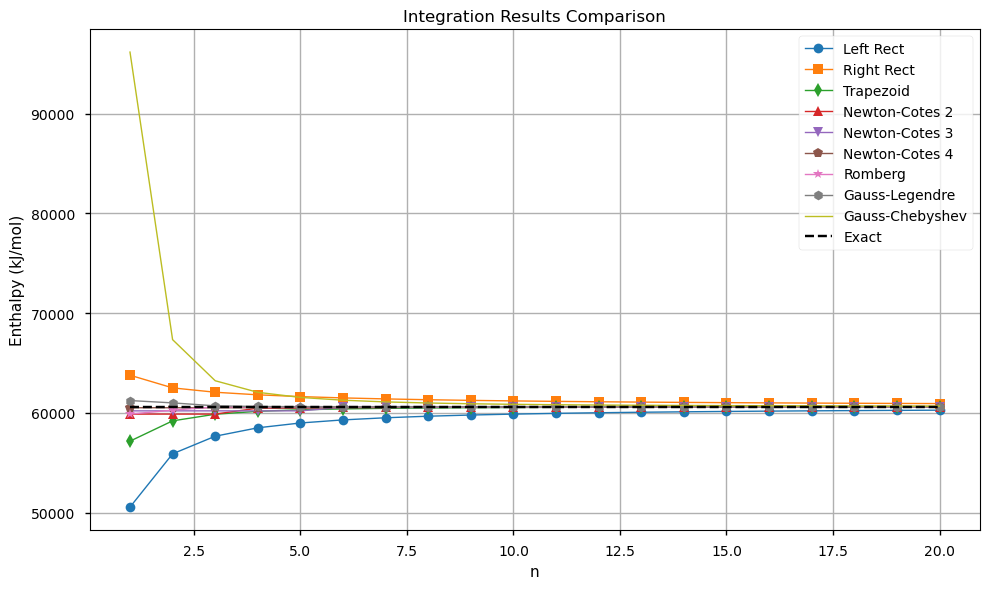
\includegraphics[width=\imagewidth\textwidth]{figures/04_int&diff/integration_results.png}
    \caption{Approximation of Integral}
\end{figure}

\begin{figure}[H]
    \centering
    \label{fig:integration_errors}
    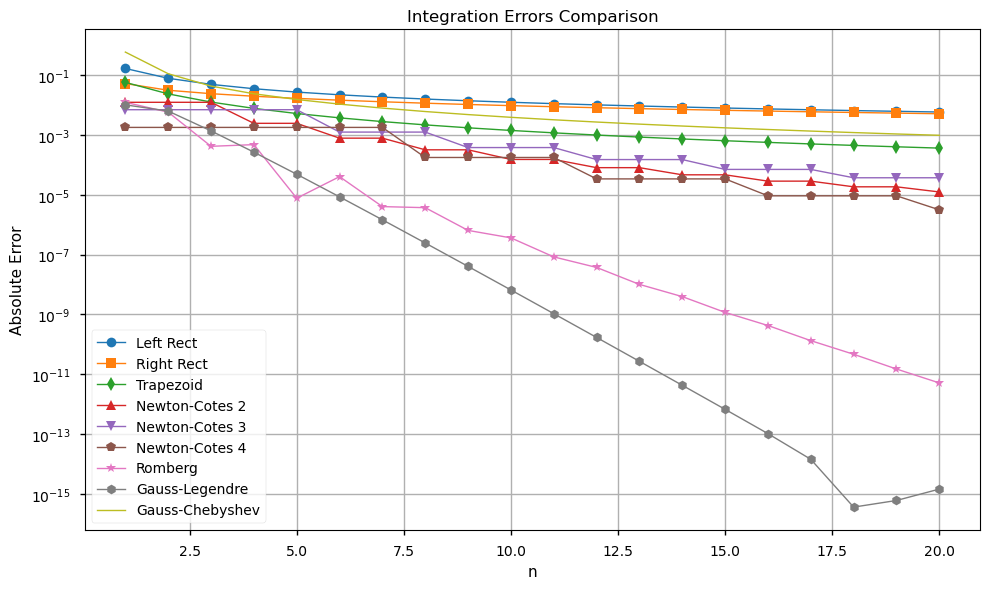
\includegraphics[width=\imagewidth\textwidth]{figures/04_int&diff/integration_errors.png}
    \caption{Error of Integral}
\end{figure}






\section{Linear Systems}
\subsection{Real Case: Copper Smelting Material Balance}






The main reaction in the Smelting Furnace is the oxidation of chalcopyrite concentrate into matte. In this stage, $\text{SiO}_2$ is used as a flux to capture impurities and regulate slag composition. The main reaction in the Smelting Furnace is:
$$
\text{CuFeS}_2(s) + \dots \text{O}_2(g) + w\text{SiO}_2(s) \rightarrow 0.5\text{Cu}_2\text{S} - x\text{FeS}(l) + (1 - x)\text{FeO} - w\text{SiO}_2(l) + \dots \text{SO}_2(g)
$$

No chemical reactions occur in the Slag Cleaning Furnace; it only separates slag and matte by heating the molten slag and matte with electrodes in an electric furnace.

\subsubsection{Assumptions for Calculations}


    
\begin{enumerate}
    \item Matte consists of $\text{Cu}_2\text{S}$ and $\text{FeS}$.
    
    \item Off-gas consists of $\text{N}_2$, $\text{SO}_2$, and $\text{CO}_2$.
    
    \item C-slag consists of $\text{Fe}_2\text{O}_3$, $\text{CaO}$, and $\text{Cu}_2\text{O}$.
    
    \item C-slag entering the S-furnace weighs 9.98 tph with 13.25\% Cu and 43.47\% Fe.
    
    \item Cl-slag consists of $\text{Fe}_2\text{SiO}_4$, $\text{Ca}_2\text{SiO}_4$, $\text{SiO}_2$, $\text{Al}_2\text{O}_3$, and $\text{Cu}_2\text{O}$.
    
    \item Minor elements in the concentrate, such as Au, Ag, Pb, As, Sb, Zn, are negligible. Au and Ag are carried to the final copper product and separated in anode slime, while other minor elements are assumed to go to slag.
\end{enumerate}


\subsubsection{Mass balance equations with known information}

\begin{enumerate}
    \item Copper Balance
    \begin{equation}
        -0.346 w_{\text{CuFeS}_2} + 0.799 w_{\text{Cu}_2\text{S}} + 0.888 w_{\text{Cu}_2\text{O}} = 1.325 \tph
    \end{equation}

    \item Iron Balance
    \begin{equation}
        -0.304 w_{\text{CuFeS}_2} - 0.466 w_{\text{FeS}_2} + 0.635 w_{\text{FeS}} + 0.548 w_{\text{Fe}_2\text{SiO}_4} = 4.347 \tph
    \end{equation}

    \item Sulfur Balance
    \begin{equation}
        -0.349 w_{\text{CuFeS}_2} - 0.535 w_{\text{FeS}_2} + 0.202 w_{\text{Cu}_2\text{S}} + 0.365 w_{\text{FeS}} + 0.501 w_{\text{SO}_2} = 0
    \end{equation}

    \item Oxygen Balance
    \begin{equation}
        -w_{\text{O}_2} (\text{blast}) + 0.157 w_{\text{Fe}_2\text{SiO}_4} + 0.112 w_{\text{Cu}_2\text{O}} + 0.500 w_{\text{SO}_2} + 0.727 w_{\text{CO}_2} = 2.035 \tph
    \end{equation}

    \item Carbon Balance
    \begin{equation}
        -w_{\text{fuel}} + 0.273 w_{\text{CO}_2} = 0
    \end{equation}

    \item SiO$_2$ Balance
    \begin{equation}
        -w_{\text{flux}} + 0.295 w_{\text{Fe}_2\text{SiO}_4} + 0.349 w_{\text{Ca}_2\text{SiO}_4} + w_{\text{SiO}_2}(\text{cl-slag}) = 17.904 \tph
    \end{equation}

    \item CaO Balance
    \begin{equation}
        0.651 w_{\text{Ca}_2\text{SiO}_4} = 4.146 \tph
    \end{equation}

    \item Al$_2$O$_3$ Balance
    \begin{equation}
        w_{\text{Al}_2\text{O}_3}(\text{cl-slag}) = 3.704 \tph
    \end{equation}

    \item Matte Grade
    \begin{equation}
        0.68 w_{\text{FeS}} - 0.119 w_{\text{Cu}_2\text{S}} = 0
    \end{equation}

    \item Fe/SiO$_2$ in Slag
    \begin{equation}
        0.241 w_{\text{Fe}_2\text{SiO}_4}(\text{cl-slag}) - 0.363 w_{\text{Ca}_2\text{SiO}_4}(\text{cl-slag}) - 1.040 w_{\text{SiO}_2}(\text{cl-slag}) = 0
    \end{equation}

    \item Cu in Slag
    \begin{equation}
        0.879 w_{\text{Cu}_2\text{O}}(\text{cl-slag}) - 0.009 w_{\text{Fe}_2\text{SiO}_4}(\text{cl-slag}) - 0.009 w_{\text{Ca}_2\text{SiO}_4}(\text{cl-slag}) - 0.009 w_{\text{SiO}_2}(\text{cl-slag}) = 0
    \end{equation}

    \item Weight of Sulfide Minerals in Concentrate
    \begin{equation}
        w_{\text{CuFeS}_2} + w_{\text{FeS}_2} = 100.013 \tph
    \end{equation}

    \item CuFeS$_2$/FeS$_2$ in Concentrate
    \begin{equation}
        0.150 w_{\text{CuFeS}_2} - 0.85 w_{\text{FeS}_2} = 0
    \end{equation}

    \item Weight of C-Slag
    \begin{equation}
        w_{\text{C-slag}} = 10 \tph
    \end{equation}

    \item Weight of Fuel
    \begin{equation}
        w_{\text{fuel}} = 1.235 \tph
    \end{equation}

    \item Total N$_2$
    \begin{equation}
        w_{\text{N}_2} = 76.64 \tph
    \end{equation}
\end{enumerate}



% \begin{sidewaysfigure}
\begin{landscape}
    

\[ \setlength\arraycolsep{1pt} % default value: 5pt 
\mathbf{A} = \left[ \begin{array}{@{} *{16}{S[table-format=-1.3, round-mode=places, round-precision=2]} @{}}
    -0.346 &  0.000 &  0.000 &  0.000 &  0.000 &  0.000 &  0.000 &  0.799 &  0.000 &  0.000 &  0.000 &  0.000 &  0.000 &  0.888 &  0.000 &  0.000 \\
    -0.304 & -0.466 &  0.000 &  0.000 &  0.000 &  0.000 &  0.000 &  0.000 &  0.635 &  0.548 &  0.000 &  0.000 &  0.000 &  0.000 &  0.000 &  0.000 \\
    -0.349 & -0.535 &  0.000 &  0.000 &  0.000 &  0.000 &  0.000 &  0.202 &  0.365 &  0.000 &  0.000 &  0.000 &  0.000 &  0.000 &  0.501 &  0.000 \\
     0.000 &  0.000 &  0.000 &  0.000 &  0.000 & -1.000 &  0.000 &  0.000 &  0.000 &  0.157 &  0.000 &  0.000 &  0.000 &  0.112 &  0.500 &  0.727 \\
     0.000 &  0.000 &  0.000 &  0.000 & -1.000 &  0.000 &  0.000 &  0.000 &  0.000 &  0.000 &  0.000 &  0.000 &  0.000 &  0.000 &  0.000 &  0.273 \\
     0.000 &  0.000 &  0.000 & -1.000 &  0.000 &  0.000 &  0.000 &  0.000 &  0.000 &  0.295 &  1.000 &  0.349 &  0.000 &  0.000 &  0.000 &  0.000 \\
     0.000 &  0.000 &  0.000 &  0.000 &  0.000 &  0.000 &  0.000 &  0.000 &  0.000 &  0.000 &  0.000 &  0.651 &  0.000 &  0.000 &  0.000 &  0.000 \\
     0.000 &  0.000 &  0.000 &  0.000 &  0.000 &  0.000 &  0.000 &  0.000 &  0.000 &  0.000 &  0.000 &  0.000 &  1.000 &  0.000 &  0.000 &  0.000 \\
     0.000 &  0.000 &  0.000 &  0.000 &  0.000 &  0.000 &  0.000 & -0.119 &  0.680 &  0.000 &  0.000 &  0.000 &  0.000 &  0.000 &  0.000 &  0.000 \\
     0.000 &  0.000 &  0.000 &  0.000 &  0.000 &  0.000 &  0.000 &  0.000 &  0.000 &  0.241 & -1.040 & -0.363 &  0.000 &  0.000 &  0.000 &  0.000 \\
     0.000 &  0.000 &  0.000 &  0.000 &  0.000 &  0.000 &  0.000 &  0.000 &  0.000 & -0.009 & -0.009 & -0.009 &  0.000 &  0.880 &  0.000 &  0.000 \\
     1.000 &  1.000 &  0.000 &  0.000 &  0.000 &  0.000 &  0.000 &  0.000 &  0.000 &  0.000 &  0.000 &  0.000 &  0.000 &  0.000 &  0.000 &  0.000 \\
     0.150 & -0.850 &  0.000 &  0.000 &  0.000 &  0.000 &  0.000 &  0.000 &  0.000 &  0.000 &  0.000 &  0.000 &  0.000 &  0.000 &  0.000 &  0.000 \\
     0.000 &  0.000 &  1.000 &  0.000 &  0.000 &  0.000 &  0.000 &  0.000 &  0.000 &  0.000 &  0.000 &  0.000 &  0.000 &  0.000 &  0.000 &  0.000 \\
     0.000 &  0.000 &  0.000 &  0.000 &  1.000 &  0.000 &  0.000 &  0.000 &  0.000 &  0.000 &  0.000 &  0.000 &  0.000 &  0.000 &  0.000 &  0.000 \\
     0.000 &  0.000 &  0.000 &  0.000 &  0.000 &  0.000 &  1.000 &  0.000 &  0.000 &  0.000 &  0.000 &  0.000 &  0.000 &  0.000 &  0.000 &  0.000 \\
\end{array} \right] \] 


\[\setlength\arraycolsep{1pt} 
\mathbf{b^T} = \left[ \begin{array}{@{} *{16}{S[table-format=-1.3, round-mode=places, round-precision=2]} @{}} 
1.325 & 4.347 & 0.000 & 2.037 & 0.000 & 17.904 & 4.143 & 3.704 & 0.000 & 0.000 & 0.000 & 100.013 & 0.000 & 10.000 & 1.235 & 76.640 \\ 
\end{array} \right] \] 

\[\setlength\arraycolsep{3.5pt} 
\mathbf{x^T} = \left[ \begin{array}{@{} *{16}{c} @{}} 
w_{\text{CuFeS}_2} & w_{\text{FeS}_2} & w_{\text{C-Slag}} & w_{\text{Flux}} & w_{\text{Fuel}} & w_{\text{O}_2} & w_{\text{N}_2} & w_{\text{Cu}_2\text{S}} & w_{\text{FeS}} & w_{\text{Fe}_2\text{SiO}_4} & w_{\text{SiO}_2} & w_{\text{Ca}_2\text{SiO}_4} & w_{\text{Al}_2\text{O}_3} & w_{\text{Cu}_2\text{O}} & w_{\text{SO}_2} & w_{\text{CO}_2} \\ 
\end{array} \right] \]

\end{landscape}



A linear system is a set of linear equations that can be written in matrix form as:
\begin{equation}
A \cdot \mathbf{x} = \mathbf{b}
\end{equation}
where $A$ is the coefficient matrix, $\mathbf{x}$ is the vector of unknowns, and $\mathbf{b}$ is the vector of constants.

\subsection{Methods}

\subsubsection{Jacobian Method}
The Jacobi method is an iterative method for solving a linear system of equations. The algorithm is as follows:
\begin{algorithm}[H]
\caption{Jacobi Method}
\begin{algorithmic}
\State $\mathbf{x}^{(0)}$, an initial guess for the solution vector\;
\For{$k = 0$ to $max\_iterations$}
    \For{$i = 0$ to $n-1$}
        \State $x_i^{(k+1)} \gets \frac{\mathbf{b}_i - \cdot \sum_{j \neq i} A_{ij} x_j^{(k)}}{A_{ii}}$;
    \EndFor
\State \textbf{return} $\mathbf{x}^{(k+1)}$;
\end{algorithmic}
\end{algorithm}
Python snippet for the Jacobian method:
\begin{lstlisting}[style=custompython][caption={Jacobian method}, label=code:jacobi]
def jacobi(A, b, max_iterations):
    n = len(b)
    x = np.zeros_like(b, dtype=np.float64)
    results = []
    results.append({'k': 0, 'x': x.copy(), 'residual': np.linalg.norm(A @ x - b)})
    
    for k in range(max_iterations):
        x_new = np.zeros_like(x)
        for i in range(n):
            sum_total = np.dot(A[i, :], x) - A[i, i] * x[i]
            x_new[i] = (b[i] - sum_total) / A[i, i]
        x = x_new.copy()
        residual = np.linalg.norm(A @ x - b)
        results.append({'k': k + 1, 'x': x.copy(), 'residual': residual})
    
    return pd.DataFrame(results)
\end{lstlisting}

\subsubsection{Gauss-Seidel Method}
The Gauss-Seidel method is another iterative method for solving a linear system. The algorithm is as follows:
\begin{algorithm}[H]
\caption{Gauss-Seidel Method}
\begin{algorithmic}
\State $\mathbf{x}^{(0)}$, an initial guess for the solution vector\;
\For{$k = 0$ to $max\_iterations$}
    \For{$i = 0$ to $n-1$}
        \State $s \gets \sum_{j=0}^{i-1} A_{ij} x_j^{(k)}$;
        \State $t \gets \sum_{j=i+1}^{n} A_{ij} x_j^{(k)}$;
        \State $x_i^{(k+1)} \gets \frac{\mathbf{b}_i - s - t}{A_{ii}}$;
    \EndFor
\State \textbf{return} $\mathbf{x}^{(k+1)}$;
\end{algorithmic}
\end{algorithm}
Python snippet for the Gauss-Seidel method:
\begin{lstlisting}[style=custompython][caption={Gauss-Seidel method}, label=code:gs]
def gauss_seidel(A, b, max_iterations):
    n = len(b)
    x = np.zeros_like(b, dtype=np.float64)
    results = []
    results.append({'k': 0, 'x': x.copy(), 'residual': np.linalg.norm(A @ x - b)})
    
    for k in range(max_iterations):
        x_new = np.zeros_like(x)
        for i in range(n):
            sum_before = np.dot(A[i, :i], x_new[:i])
            sum_after = np.dot(A[i, i+1:], x[i+1:])
            x_new[i] = (b[i] - sum_before - sum_after) / A[i, i]
        x = x_new.copy()
        residual = np.linalg.norm(A @ x - b)
        results.append({'k': k + 1, 'x': x.copy(), 'residual': residual})
    
    return pd.DataFrame(results)
\end{lstlisting}


\subsubsection{SOR Method}
The SOR (Successive Over-Relaxation) method is an iterative method for solving a linear system. The algorithm is as follows:
\begin{algorithm}[H]
\caption{SOR Method}
\begin{algorithmic}
\State $\mathbf{x}^{(0)}$, an initial guess for the solution vector\;
\For{$k = 0$ to $max\_iterations$}
    \For{$i = 0$ to $n-1$}
        \State $w \gets \mathbf{b}_i - \cdot \sum_{j=0}^{i-1} A_{ij} x_j^{(k)}$;
        \State $u \gets \mathbf{b}_i - \cdot \sum_{j=i+1}^{n} A_{ij} x_j^{(k)}$;
        \State $x_i^{(k+1)} \gets (1-w) x_i^{(k)} + w$;
    \EndFor
\State \textbf{return} $\mathbf{x}^{(k+1)}$;
\end{algorithmic}
\end{algorithm}

Python snippet for the SOR method:
\begin{lstlisting}[style=custompython][caption={SOR method}, label=code:sor]
def SOR(A, b, max_iterations, w):
    n = len(b)
    x = np.zeros_like(b, dtype=np.float64)
    results = []
    results.append({'k': 0, 'x': x.copy(), 'residual': np.linalg.norm(A @ x - b)})
    
    for k in range(max_iterations):
        x_new = np.zeros_like(x)
        for i in range(n):
            sum_before = np.dot(A[i, :i], x_new[:i])
            sum_after = np.dot(A[i, i+1:], x[i+1:])
            x_new[i] = (1 - w) * x[i] + w * (b[i] - sum_before - sum_after) / A[i, i]
        x = x_new.copy()
        residual = np.linalg.norm(A @ x - b)
        results.append({'k': k + 1, 'x': x.copy(), 'residual': residual})
    
    return pd.DataFrame(results)
\end{lstlisting}


\subsubsection{Steepest Descent Method}
The Steepest Descent method is an iterative method for solving a linear system. The algorithm is as follows:
\begin{algorithm}[H]
\caption{Steepest Descent Method}
\begin{algorithmic}
\State $\mathbf{x}^{(0)}$, an initial guess for the solution vector\;
\State $\mathbf{r}^{(0)} \gets \mathbf{b} - A \cdot \mathbf{x}^{(0)}$;
\State $\mathbf{residuals}^{(0)} \gets \lVert \mathbf{r}^{(0)} \rVert$;
\For{$k = 1$ to $max\_iterations$}
    \State $\mathbf{Ar} \gets A \cdot \mathbf{r}^{(k-1)}$;
    \State $\alpha \gets \frac{\mathbf{r}^{(k-1)} \cdot \mathbf{r}^{(k-1)}}{\mathbf{r}^{(k-1)} \cdot \mathbf{Ar}^{(k-1)}}$;
    \State $\mathbf{x}^{(k)} \gets \mathbf{x}^{(k-1)} + \alpha \cdot \mathbf{r}^{(k-1)}$;
    \State $\mathbf{r}^{(k)} \gets \mathbf{r}^{(k-1)} - \alpha \cdot \mathbf{Ar}^{(k-1)}$;
    \State $\mathbf{residuals}^{(k)} \gets \lVert \mathbf{r}^{(k)} \rVert$;
\EndFor
\State \textbf{return} $\mathbf{x}^{(k)}$;
\end{algorithmic}
\end{algorithm}
Python snippet for the Steepest Descent method:
\begin{lstlisting}[style=custompython][caption={Steepest Descent method}, label=code:sd]
def steepest_descent(A, b, max_iterations):
    x = np.zeros_like(b, dtype=np.float64)
    r = b - A @ x
    residuals = [np.linalg.norm(r)]
    results = []
    results.append({
        'k': 0,
        'x': x.copy(),
        'p': r.copy(),
        'alpha': np.nan,
        'residual': residuals[0]
    })
    
    for k in range(max_iterations):
        Ar = A @ r
        alpha = np.dot(r, r) / np.dot(r, Ar)
        x = x + alpha * r
        r = r - alpha * Ar
        residual = np.linalg.norm(r)
        residuals.append(residual)
        results.append({
            'k': k + 1,
            'x': x.copy(),
            'p': r.copy(),
            'alpha': alpha,
            'residual': residual
        })
    
    return pd.DataFrame(results)
\end{lstlisting}


\subsubsection{Conjugate Gradient Method}
The Conjugate Gradient method is an iterative method for solving a linear system. The algorithm is as follows:
\begin{algorithm}[H]
\caption{Conjugate Gradient Method}
\begin{algorithmic}
\State $\mathbf{x}^{(0)}$, an initial guess for the solution vector\;
\State $\mathbf{r}^{(0)} \gets \mathbf{b} - A \cdot \mathbf{x}^{(0)}$;
\State $\mathbf{p}^{(0)} \gets \mathbf{r}^{(0)}$;
\For{$k = 1$ to $max\_iterations$}
    \State $\mathbf{Ap} \gets A \cdot \mathbf{p}^{(k-1)}$;
    \State $\alpha \gets \frac{\mathbf{r}^{(k-1)} \cdot \mathbf{r}^{(k-1)}}{\mathbf{r}^{(k-1)} \cdot \mathbf{Ap}^{(k-1)}}$;
    \State $\mathbf{x}^{(k)} \gets \mathbf{x}^{(k-1)} + \alpha \cdot \mathbf{p}^{(k-1)}$;
    \State $\mathbf{r}^{(k)} \gets \mathbf{r}^{(k-1)} - \alpha \cdot \mathbf{Ap}^{(k-1)}$;
    \State $\mathbf{beta} \gets \frac{\mathbf{r}^{(k)} \cdot \mathbf{r}^{(k)}}{\mathbf{r}^{(k-1)} \cdot \mathbf{r}^{(k-1)}}$;
    \State $\mathbf{p}^{(k)} \gets \mathbf{r}^{(k)} + \beta \cdot \mathbf{p}^{(k-1)}$;
\EndFor
\State \textbf{return} $\mathbf{x}^{(k)}$;
\end{algorithmic}
\end{algorithm}

Python snippet for the Conjugate Gradient method:
\begin{lstlisting}[style=custompython][caption={Conjugate Gradient method}, label=code:cg]
def conjugate_gradient(A, b, max_iterations):
    x = np.zeros_like(b, dtype=np.float64)
    r = b - A @ x
    p = r.copy()
    residuals = [np.linalg.norm(r)]
    results = []
    results.append({
        'k': 0,
        'x': x.copy(),
        'p': p.copy(),
        'r': r.copy(),
        'alpha': np.nan,
        'beta': np.nan,
        'residual': residuals[0]
    })
    
    for k in range(max_iterations):
        Ap = A @ p
        alpha = np.dot(r, r) / np.dot(p, Ap)
        x = x + alpha * p
        r_new = r - alpha * Ap
        residual = np.linalg.norm(r_new)
        residuals.append(residual)
        beta = np.dot(r_new, r_new) / np.dot(r, r)
        p = r_new + beta * p
        results.append({
            'k': k + 1,
            'x': x.copy(),
            'p': p.copy(),
            'r': r_new.copy(),
            'alpha': alpha,
            'beta': beta,
            'residual': residual
        })
        r = r_new
    
    return pd.DataFrame(results)
\end{lstlisting}

\subsection{Python snippet for various method comparison}
\begin{lstlisting}[style=custompython][caption={Linear system method comparison}, label=code:lscomparison]
\begin{lstlisting}[style=custompython]
import numpy as np
import pandas as pd
import os
from scipy.optimize import linear_sum_assignment
import matplotlib.pyplot as plt

# Matrix preprocessing to create diagonally dominant matrix
def make_diagonally_dominant(A, b):
    n = len(b)
    A_new = A.copy()
    b_new = b.copy()
    col_order = np.arange(n)
    
    for i in range(n):
        if A_new[i, i] == 0:
            for j in range(i + 1, n):
                if A_new[j, i] != 0:
                    A_new[[i, j]] = A_new[[j, i]]
                    b_new[[i, j]] = b_new[[j, i]]
                    break
            for k in range(i + 1, n):
                if A_new[i, k] != 0:
                    A_new[:, [i, k]] = A_new[:, [k, i]]
                    col_order[[i, k]] = col_order[[k, i]]
                    break
    
    cost = -np.abs(A_new)
    row_ind, col_ind = linear_sum_assignment(cost)
    A_new = A_new[row_ind][:, col_ind]
    b_new = b_new[row_ind]
    col_order = col_order[col_ind]
    
    return A_new, b_new, col_order

# Jacobi method
def jacobi(A, b, max_iterations):
    n = len(b)
    x = np.zeros_like(b, dtype=np.float64)
    results = []
    results.append({'k': 0, 'x': x.copy(), 'residual': np.linalg.norm(A @ x - b)})
    
    for k in range(max_iterations):
        x_new = np.zeros_like(x)
        for i in range(n):
            sum_total = np.dot(A[i, :], x) - A[i, i] * x[i]
            x_new[i] = (b[i] - sum_total) / A[i, i]
        x = x_new.copy()
        residual = np.linalg.norm(A @ x - b)
        results.append({'k': k + 1, 'x': x.copy(), 'residual': residual})
    
    return pd.DataFrame(results)

# Gauss-Seidel method
def gauss_seidel(A, b, max_iterations):
    n = len(b)
    x = np.zeros_like(b, dtype=np.float64)
    results = []
    results.append({'k': 0, 'x': x.copy(), 'residual': np.linalg.norm(A @ x - b)})
    
    for k in range(max_iterations):
        x_new = np.zeros_like(x)
        for i in range(n):
            sum_before = np.dot(A[i, :i], x_new[:i])
            sum_after = np.dot(A[i, i+1:], x[i+1:])
            x_new[i] = (b[i] - sum_before - sum_after) / A[i, i]
        x = x_new.copy()
        residual = np.linalg.norm(A @ x - b)
        results.append({'k': k + 1, 'x': x.copy(), 'residual': residual})
    
    return pd.DataFrame(results)

# SOR method
def SOR(A, b, max_iterations, w):
    n = len(b)
    x = np.zeros_like(b, dtype=np.float64)
    results = []
    results.append({'k': 0, 'x': x.copy(), 'residual': np.linalg.norm(A @ x - b)})
    
    for k in range(max_iterations):
        x_new = np.zeros_like(x)
        for i in range(n):
            sum_before = np.dot(A[i, :i], x_new[:i])
            sum_after = np.dot(A[i, i+1:], x[i+1:])
            x_new[i] = (1 - w) * x[i] + w * (b[i] - sum_before - sum_after) / A[i, i]
        x = x_new.copy()
        residual = np.linalg.norm(A @ x - b)
        results.append({'k': k + 1, 'x': x.copy(), 'residual': residual})
    
    return pd.DataFrame(results)

# Steepest Descent method
def steepest_descent(A, b, max_iterations):
    x = np.zeros_like(b, dtype=np.float64)
    r = b - A @ x
    residuals = [np.linalg.norm(r)]
    results = []
    results.append({
        'k': 0,
        'x': x.copy(),
        'p': r.copy(),
        'alpha': np.nan,
        'residual': residuals[0]
    })
    
    for k in range(max_iterations):
        Ar = A @ r
        alpha = np.dot(r, r) / np.dot(r, Ar)
        x = x + alpha * r
        r = r - alpha * Ar
        residual = np.linalg.norm(r)
        residuals.append(residual)
        results.append({
            'k': k + 1,
            'x': x.copy(),
            'p': r.copy(),
            'alpha': alpha,
            'residual': residual
        })
    
    return pd.DataFrame(results)

# Conjugate Gradient method
def conjugate_gradient(A, b, max_iterations):
    x = np.zeros_like(b, dtype=np.float64)
    r = b - A @ x
    p = r.copy()
    residuals = [np.linalg.norm(r)]
    results = []
    results.append({
        'k': 0,
        'x': x.copy(),
        'p': p.copy(),
        'r': r.copy(),
        'alpha': np.nan,
        'beta': np.nan,
        'residual': residuals[0]
    })
    
    for k in range(max_iterations):
        Ap = A @ p
        alpha = np.dot(r, r) / np.dot(p, Ap)
        x = x + alpha * p
        r_new = r - alpha * Ap
        residual = np.linalg.norm(r_new)
        residuals.append(residual)
        beta = np.dot(r_new, r_new) / np.dot(r, r)
        p = r_new + beta * p
        results.append({
            'k': k + 1,
            'x': x.copy(),
            'p': p.copy(),
            'r': r_new.copy(),
            'alpha': alpha,
            'beta': beta,
            'residual': residual
        })
        r = r_new
    
    return pd.DataFrame(results)

# Matrix and vector definitions
A = np.array([...])  # Matrix definition
b = np.array([...])  # Vector definition
variables = [...]     # Variable names

# Parameters
w = 0.965
max_iterations = 10

# Preprocessing
A_new, b_new, col_order = make_diagonally_dominant(A, b)
inv_col_order = np.argsort(col_order)

# Run methods
jacob_result = jacobi(A_new, b_new, max_iterations)
gs_result = gauss_seidel(A_new, b_new, max_iterations)
sor_result = SOR(A_new, b_new, max_iterations, w)
sd_result = steepest_descent(A, b, max_iterations)
cg_result = conjugate_gradient(A, b, max_iterations)

# Process and save results
output_dir = "06_linearsys/results"
os.makedirs(output_dir, exist_ok=True)

with pd.ExcelWriter(os.path.join(output_dir, "linear_system_results.xlsx")) as writer:
    jacob_result.to_excel(writer, sheet_name='Jacobi', index=False)
    gs_result.to_excel(writer, sheet_name='Gauss-Seidel', index=False)
    sor_result.to_excel(writer, sheet_name='SOR', index=False)
    sd_result.to_excel(writer, sheet_name='Steepest-Descent', index=False)
    cg_result.to_excel(writer, sheet_name='Conjugate-Gradient', index=False)

# Plot residuals comparison
def plot_residuals_comparison(error_df, output_dir):
    markerss = ['o', 's', 'd', '^', 'v', 'p', '*', 'h', '+', 'x']
    plt.figure(figsize=(10, 6))
    plt.style.use('seaborn-v0_8-notebook')
    for i, column in enumerate(error_df.columns):
        plt.semilogy(error_df.index, error_df[column], marker=markerss[i], label=column)
    plt.title('Residuals Comparison of Different Methods')
    plt.xlabel('Iteration')
    plt.ylabel('Residual')
    plt.legend()
    plt.grid(True)
    plt.savefig(os.path.join(output_dir, "residuals_comparison.png"))
    plt.show()

# Generate and display residuals comparison
error = pd.DataFrame({
    'Jacobi': jacob_result['residual'],
    'Gauss-Seidel': gs_result['residual'],
    'SOR': sor_result['residual'],
    'Steepest-Descent': sd_result['residual'],
    'Conjugate-Gradient': cg_result['residual']
})
error.index = jacob_result['k']

print("Residuals Comparison:")
print(error.to_string())
plot_residuals_comparison(error, output_dir)

\end{lstlisting}



\subsection{Results}

\subsubsection{Jacobian Method}

\begin{table}[H]
\centering
\caption{Results of Jacobian method (Part 1)}
\begin{tabular}{ccccccccccc}
\toprule
\( k \) & \( w_{\text{CuFeS2}} \) & \( w_{\text{FeS2}} \) & \( w_{\text{C\_Slag}} \) & \( w_{\text{Flux}} \) & \( w_{\text{Fuel}} \) & \( w_{\text{O2}} \) & \( w_{\text{N2}} \) & \( w_{\text{Cu2S}} \) & \( w_{\text{FeS}} \)\\
\midrule
0 & 0.0000 & 0.0000 & 0.0000 & 0.0000 & 0.0000 & 0.0000 & 0.0000 & 0.0000 & 0.0000 \\
1 & 100.0130 & 0.0000 & 10.0000 & -17.9040 & 1.2350 & -2.0370 & 76.6400 & 1.6583 & 0.0000 \\
2 & 100.0130 & 17.6494 & 10.0000 & -13.3429 & 1.2350 & -0.7916 & 76.6400 & 44.9681 & 0.2902\\
3 & 82.3636 & 17.6494 & 10.0000 & 2.6411 & 1.2350 & 45.7248 & 76.6400 & 44.8056 & 7.8694 \\
4 & 82.3636 & 14.5348 & 10.0000 & 19.8262 & 1.2350 & 48.6781 & 76.6400 & 36.5364 & 7.8410 \\
5 & 85.4782 & 14.5348 & 10.0000 & 17.7470 & 1.2350 & 36.9182 & 76.6400 & 36.2235 & 6.3939 \\
6 & 85.4782 & 15.0844 & 10.0000 & 12.6714 & 1.2350 & 36.5046 & 76.6400 & 37.7447 & 6.3391 \\
7 & 84.9286 & 15.0844 & 10.0000 & 13.0697 & 1.2350 & 38.7062 & 76.6400 & 37.8234 & 6.6053 \\
8 & 84.9286 & 14.9874 & 10.0000 & 14.0153 & 1.2350 & 38.7995 & 76.6400 & 37.5535 & 6.6191 \\
9 & 85.0256 & 14.9874 & 10.0000 & 13.9573 & 1.2350 & 38.4005 & 76.6400 & 37.5385 & 6.5719 \\
10 & 85.0256 & 15.0045 & 10.0000 & 13.7861 & 1.2350 & 38.3820 & 76.6400 & 37.5861 & 6.5692 \\
\bottomrule
\end{tabular}
\end{table}

\begin{table}[H]
\centering
\caption{Results of Jacobian method (Part 2)}
\begin{tabular}{ccccccccccc}
\toprule
\( k \) & \( w_{\text{Fe2SiO4}} \) & \( w_{\text{SiO2}} \) & \( w_{\text{Ca2SiO4}} \) & \( w_{\text{Al2O3}} \) & \( w_{\text{Cu2O}} \) & \( w_{\text{SO2}} \) & \( w_{\text{CO2}} \) & Residual \\
\midrule
0 & 0.0000 & 0.0000 & 0.0000 & 0.0000 & 0.0000 & 0.0000 & 0.0000 & 127.8830 \\
1 & 7.9325 & 0.0000 & 6.3641 & 3.7040 & 0.0000 & 0.0000 & 0.0000 & 59.7167 \\
2 & 63.4141 & -0.3831 & 6.3641 & 3.7040 & 0.1462 & 69.0011 & 4.5238 & 54.7847 \\
3 & 78.0863 & 12.4737 & 6.3641 & 3.7040 & 0.7097 & 70.1746 & 4.5238 & 23.4513 \\
4 & 59.5129 & 15.8737 & 6.3641 & 3.7040 & 0.9913 & 52.4237 & 4.5238 & 13.2461 \\
5 & 56.8973 & 11.5697 & 6.3641 & 3.7040 & 0.8361 & 52.4525 & 4.5238 & 5.8591 \\
6 & 60.3020 & 10.9636 & 6.3641 & 3.7040 & 0.7653 & 55.8026 & 4.5238 & 2.4705 \\
7 & 60.8328 & 11.7525 & 6.3641 & 3.7040 & 0.7939 & 55.8161 & 4.5238 & 1.0856 \\
8 & 60.2194 & 11.8755 & 6.3641 & 3.7040 & 0.8074 & 55.2075 & 4.5238 & 0.4449 \\
9 & 60.1210 & 11.7334 & 6.3641 & 3.7040 & 0.8024 & 55.2027 & 4.5238 & 0.1958 \\
10 & 60.2295 & 11.7106 & 6.3641 & 3.7040 & 0.7999 & 55.3107 & 4.5238 & 0.0787 \\
\bottomrule
\end{tabular}
\end{table}





\subsubsection{Gauss-Seidel Method}

\begin{table}[H]
\centering
\caption{Results of Gauss-Seidel method (Part 1)}
\begin{tabular}{ccccccccccc}
\toprule
\( k \) & \( w_{\text{CuFeS2}} \) & \( w_{\text{FeS2}} \) & \( w_{\text{C\_Slag}} \) & \( w_{\text{Flux}} \) & \( w_{\text{Fuel}} \) & \( w_{\text{O2}} \) & \( w_{\text{N2}} \) & \( w_{\text{Cu2S}} \) & \( w_{\text{FeS}} \) \\
\midrule
0 & 0.0000 & 0.0000 & 0.0000 & 0.0000 & 0.0000 & 0.0000 & 0.0000 & 0.0000 & 0.0000 \\
1 & 100.0130 & 17.6494 & 10.0000 & -15.5639 & 1.2350 & -0.7916 & 76.6400 & 1.6583 & 0.2902 \\
2 & 82.3636 & 14.5348 & 10.0000 & 9.1907 & 1.2350 & 13.0825 & 76.6400 & 44.8570 & 7.8499 \\
3 & 85.4782 & 15.0844 & 10.0000 & 16.9724 & 1.2350 & 42.6538 & 76.6400 & 36.1849 & 6.3323 \\
4 & 84.9286 & 14.9874 & 10.0000 & 13.2262 & 1.2350 & 37.7355 & 76.6400 & 37.8304 & 6.6203 \\
5 & 85.0256 & 15.0045 & 10.0000 & 13.9297 & 1.2350 & 38.5695 & 76.6400 & 37.5370 & 6.5690 \\
6 & 85.0085 & 15.0015 & 10.0000 & 13.8003 & 1.2350 & 38.4232 & 76.6400 & 37.5891 & 6.5781 \\
7 & 85.0115 & 15.0020 & 10.0000 & 13.8232 & 1.2350 & 38.4489 & 76.6400 & 37.5799 & 6.5765 \\
8 & 85.0110 & 15.0019 & 10.0000 & 13.8192 & 1.2350 & 38.4443 & 76.6400 & 37.5816 & 6.5768 \\
9 & 85.0111 & 15.0020 & 10.0000 & 13.8199 & 1.2350 & 38.4451 & 76.6400 & 37.5813 & 6.5767 \\
10 & 85.0110 & 15.0020 & 10.0000 & 13.8198 & 1.2350 & 38.4450 & 76.6400 & 37.5813 & 6.5767 \\
\bottomrule
\end{tabular}
\end{table}

\begin{table}[H]
\centering
\caption{Results of Gauss-Seidel method (Part 2)}
\begin{tabular}{ccccccccccc}
\toprule
\( k \) & \( w_{\text{Fe2SiO4}} \) & \( w_{\text{SiO2}} \) & \( w_{\text{Ca2SiO4}} \) & \( w_{\text{Al2O3}} \) & \( w_{\text{Cu2O}} \) & \( w_{\text{SO2}} \) & \( w_{\text{CO2}} \) & Residual \\
\midrule
0 & 0.0000 & 0.0000 & 0.0000 & 0.0000 & 0.0000 & 0.0000 & 0.0000 & 127.8830 \\
1 & 7.9325 & 1.8382 & 6.3641 & 3.7040 & 0.0999 & -0.8801 & 0.0000 & 70.5052 \\
2 & 78.0863 & 15.8737 & 6.3641 & 3.7040 & 1.0260 & 64.7117 & 4.5238 & 39.1574 \\
3 & 56.8869 & 10.9611 & 6.3641 & 3.7040 & 0.7590 & 53.6933 & 4.5238 & 7.9654 \\
4 & 60.8406 & 11.8773 & 6.3641 & 3.7040 & 0.8088 & 55.5766 & 4.5238 & 1.4201 \\
5 & 60.1196 & 11.7103 & 6.3641 & 3.7040 & 0.7997 & 55.2459 & 4.5238 & 0.2538 \\
6 & 60.2474 & 11.7399 & 6.3641 & 3.7040 & 0.8013 & 55.3041 & 4.5238 & 0.0448 \\
7 & 60.2248 & 11.7346 & 6.3641 & 3.7040 & 0.8010 & 55.2938 & 4.5238 & 0.0079 \\
8 & 60.2288 & 11.7356 & 6.3641 & 3.7040 & 0.8011 & 55.2956 & 4.5238 & 0.0014 \\
9 & 60.2281 & 11.7354 & 6.3641 & 3.7040 & 0.8011 & 55.2953 & 4.5238 & 0.0002 \\
10 & 60.2282 & 11.7354 & 6.3641 & 3.7040 & 0.8011 & 55.2954 & 4.5238 & 0.0000 \\
\bottomrule
\end{tabular}
\end{table}



\subsubsection{SOR Method}

\begin{table}[H]
\centering
\caption{Results of SOR method (Part 1)}
\begin{tabular}{ccccccccccc}
\toprule
\( k \) & \( w_{\text{CuFeS2}} \) & \( w_{\text{FeS2}} \) & \( w_{\text{C\_Slag}} \) & \( w_{\text{Flux}} \) & \( w_{\text{Fuel}} \) & \( w_{\text{O2}} \) & \( w_{\text{N2}} \) & \( w_{\text{Cu2S}} \) & \( w_{\text{FeS}} \) \\
\midrule
0 & 0.0000 & 0.0000 & 0.0000 & 0.0000 & 0.0000 & 0.0000 & 0.0000 & 0.0000 & 0.0000 \\
1 & 96.5125 & 16.4355 & 9.6500 & -15.0982 & 1.1918 & -0.8060 & 73.9576 & 1.6003 & 0.2702 \\
2 & 84.0302 & 14.8851 & 9.9878 & 6.6312 & 1.2335 & 11.6050 & 76.5461 & 41.8883 & 7.0833 \\
3 & 85.0895 & 15.0112 & 9.9996 & 15.7936 & 1.2349 & 39.9094 & 76.6367 & 37.1916 & 6.5286 \\
4 & 85.0049 & 15.0012 & 9.9999 & 13.8372 & 1.2350 & 38.3083 & 76.6399 & 37.6047 & 6.5790 \\
5 & 85.0115 & 15.0020 & 10.0000 & 13.8335 & 1.2350 & 38.4577 & 76.6400 & 37.5787 & 6.5764 \\
6 & 85.0110 & 15.0019 & 10.0000 & 13.8201 & 1.2350 & 38.4444 & 76.6400 & 37.5814 & 6.5767 \\
7 & 85.0111 & 15.0020 & 10.0000 & 13.8199 & 1.2350 & 38.4451 & 76.6400 & 37.5813 & 6.5767 \\
8 & 85.0110 & 15.0020 & 10.0000 & 13.8198 & 1.2350 & 38.4450 & 76.6400 & 37.5813 & 6.5767 \\
9 & 85.0111 & 15.0020 & 10.0000 & 13.8198 & 1.2350 & 38.4450 & 76.6400 & 37.5813 & 6.5767 \\
10 & 85.0110 & 15.0020 & 10.0000 & 13.8198 & 1.2350 & 38.4450 & 76.6400 & 37.5813 & 6.5767 \\
\bottomrule
\end{tabular}
\end{table}

\begin{table}[htbp]
\centering
\caption{Results of SOR method (Part 2)}
\begin{tabular}{ccccccccccc}
\toprule
\( k \) & \( w_{\text{Fe2SiO4}} \) & \( w_{\text{SiO2}} \) & \( w_{\text{Ca2SiO4}} \) & \( w_{\text{Al2O3}} \) & \( w_{\text{Cu2O}} \) & \( w_{\text{SO2}} \) & \( w_{\text{CO2}} \) & Residual \\
\midrule
0 & 0.0000 & 0.0000 & 0.0000 & 0.0000 & 0.0000 & 0.0000 & 0.0000 & 127.8830 \\
1 & 7.6548 & 1.7118 & 6.1413 & 3.5744 & 0.0924 & -0.8126 & 0.0000 & 66.8977 \\
2 & 72.7735 & 14.2650 & 6.3563 & 3.6995 & 0.9229 & 60.5085 & 4.2127 & 35.2671 \\
3 & 59.4798 & 11.6592 & 6.3638 & 3.7038 & 0.7971 & 54.8835 & 4.5076 & 2.9772 \\
4 & 60.3054 & 11.7501 & 6.3640 & 3.7040 & 0.8018 & 55.3325 & 4.5231 & 0.1778 \\
5 & 60.2244 & 11.7351 & 6.3641 & 3.7040 & 0.8011 & 55.2930 & 4.5238 & 0.0213 \\
6 & 60.2288 & 11.7355 & 6.3641 & 3.7040 & 0.8011 & 55.2956 & 4.5238 & 0.0009 \\
7 & 60.2282 & 11.7354 & 6.3641 & 3.7040 & 0.8011 & 55.2953 & 4.5238 & 0.0002 \\
8 & 60.2282 & 11.7354 & 6.3641 & 3.7040 & 0.8011 & 55.2953 & 4.5238 & 0.0000 \\
9 & 60.2282 & 11.7354 & 6.3641 & 3.7040 & 0.8011 & 55.2953 & 4.5238 & 0.0000 \\
10 & 60.2282 & 11.7354 & 6.3641 & 3.7040 & 0.8011 & 55.2953 & 4.5238 & 0.0000 \\
\bottomrule
\end{tabular}
\end{table}


\subsubsection{Steepest Descent Method}

\begin{table}[H]
\centering
\caption{Results of Steepest Descent method (Part 1)}
\begin{tabular}{ccccccc}
\toprule
\( k \) & \( w_{\text{CuFeS2}} \) & \( w_{\text{FeS2}} \) & \( w_{\text{C\_Slag}} \) & \( w_{\text{Flux}} \) & \( w_{\text{Fuel}} \) & \( w_{\text{O2}} \) \\
\midrule
0 & 0.0000 & 0.0000 & 0.0000 & 0.0000 & 0.0000 & 0.0000 \\
1 & 1.19 \times 10^1 & 3.89 \times 10^1 & 0.0000 & 1.82 \times 10^1 & 0.0000 & 1.60 \times 10^2 \\
2 & 2.67 \times 10^2 & -2.73 \times 10^1 & -3.23 \times 10^1 & 9.12 \times 10^2 & 4.75 \times 10^2 & 8.61 \times 10^2 \\
3 & 1.79 \times 10^2 & -2.65 \times 10^3 & -3.95 \times 10^2 & -1.84 \times 10^3 & -1.08 \times 10^3 & -2.72 \times 10^3 \\
4 & -4.03 \times 10^3 & -1.20 \times 10^4 & 2.01 \times 10^4 & 7.20 \times 10^4 & 2.56 \times 10^4 & 1.05 \times 10^4 \\
5 & -2.13 \times 10^3 & 4.62 \times 10^3 & 2.97 \times 10^3 & 2.96 \times 10^4 & 7.80 \times 10^4 & 3.19 \times 10^5 \\
% 6 & -3.49 \times 10^5 & -4.69 \times 10^4 & -1.83 \times 10^5 & -1.07 \times 10^6 & -1.47 \times 10^5 & 2.73 \times 10^5 \\
% 7 & -2.20 \times 10^6 & 5.10 \times 10^6 & 1.27 \times 10^7 & -8.66 \times 10^6 & 1.25 \times 10^7 & 5.73 \times 10^7 \\
% 8 & -4.24 \times 10^7 & 2.16 \times 10^7 & -9.69 \times 10^6 & -2.03 \times 10^8 & -2.30 \times 10^7 & 5.18 \times 10^7 \\
% 9 & -3.45 \times 10^8 & -3.08 \times 10^8 & -1.80 \times 10^8 & -1.31 \times 10^8 & -2.33 \times 10^8 & -1.30 \times 10^9 \\
% 10 & 1.71 \times 10^{10} & -6.09 \times 10^8 & 2.21 \times 10^{10} & 9.29 \times 10^{10} & 1.95 \times 10^{10} & -1.24 \times 10^{10} \\
\bottomrule
\end{tabular}
\end{table}

\begin{table}[H]
\centering
\caption{Results of Steepest Descent method (Part 2)}
\begin{tabular}{ccccccc}
\toprule
\( k \) & \( w_{\text{Cu2S}} \) & \( w_{\text{FeS}} \) & \( w_{\text{Fe2SiO4}} \) & \( w_{\text{SiO2}} \) & \( w_{\text{Ca2SiO4}} \) & \( w_{\text{Al2O3}} \) \\
\midrule
0 & 0.0000 & 0.0000 & 0.0000 & 0.0000 & 0.0000 & 0.0000 \\
1 & 3.31 \times 10^1 & 0.0000 & 0.0000 & 0.0000 & 8.95 \times 10^2 & 0.0000 \\
2 & 2.37 \times 10^1 & -1.00 \times 10^1 & 1.79 \times 10^2 & 7.70 \times 10^2 & -7.94 \times 10^1 & 6.41 \times 10^1 \\
3 & -3.87 \times 10^2 & -5.76 \times 10^1 & 1.46 \times 10^3 & 2.33 \times 10^2 & -1.45 \times 10^2 & 2.35 \times 10^3 \\
4 & 1.54 \times 10^3 & 1.90 \times 10^{-1} & -2.02 \times 10^4 & 1.94 \times 10^4 & -3.55 \times 10^3 & -6.77 \times 10^3 \\
5 & -6.83 \times 10^4 & 6.61 \times 10^2 & 3.79 \times 10^4 & -1.52 \times 10^4 & -7.58 \times 10^4 & -9.89 \times 10^4 \\
% 6 & -1.12 \times 10^5 & 2.53 \times 10^4 & -1.82 \times 10^5 & 4.48 \times 10^4 & -2.73 \times 10^4 & -6.73 \times 10^4 \\
% 7 & -1.91 \times 10^6 & 2.03 \times 10^6 & -2.60 \times 10^7 & -8.52 \times 10^5 & -1.21 \times 10^7 & -9.56 \times 10^6 \\
% 8 & -4.89 \times 10^6 & 7.64 \times 10^6 & -1.58 \times 10^8 & -1.72 \times 10^7 & 3.24 \times 10^7 & 3.43 \times 10^7 \\
% 9 & 7.70 \times 10^7 & -3.67 \times 10^7 & 1.44 \times 10^8 & 1.72 \times 10^8 & 1.07 \times 10^8 & 2.11 \times 10^8 \\
% 10 & 7.13 \times 10^9 & -2.25 \times 10^9 & 1.44 \times 10^{10} & 1.72 \times 10^{10} & 1.07 \times 10^{10} & 2.11 \times 10^{10} \\
\bottomrule
\end{tabular}
\end{table}


\begin{table}[H]
\centering
\caption{Results of Steepest Descent method (Part 3)}
\begin{tabular}{ccccccc}
\toprule
\( k \) & \( w_{\text{SO2}} \) & \( w_{\text{CO2}} \) & \( \alpha \) & \( \beta \) & Residual \\
\midrule
0 & 0.0000 & 0.0000 &  &  & 1.28 \times 10^2 \\
1 & 1.10 \times 10^1 & 6.86 \times 10^2 & 8.95 \times 10^0 &  & 8.34 \times 10^2 \\
2 & -4.08 \times 10^2 & -6.78 \times 10^1 & -4.08 \times 10^2 & 5.97 \times 10^{-1} & 6.45 \times 10^2 \\
3 & 7.59 \times 10^1 & 2.52 \times 10^2 & 2.52 \times 10^2 & 1.99 \times 10^{-1} & 2.88 \times 10^2 \\
4 & -1.47 \times 10^4 & 5.00 \times 10^3 & -2.44 \times 10^3 & -1.19 \times 10^2 & 3.01 \times 10^4 \\
5 & 1.54 \times 10^4 & -4.45 \times 10^3 & 2.52 \times 10^3 & 1.16 \times 10^{-2} & 3.11 \times 10^4 \\
% 6 & -1.76 \times 10^2 & 5.88 \times 10^2 & -5.07 \times 10^1 & -5.61 \times 10^{-3} & 8.02 \times 10^2 \\
% 7 & 5.57 \times 10^2 & 3.21 \times 10^1 & 3.21 \times 10^1 & 2.08 \times 10^{-1} & 7.18 \times 10^2 \\
% 8 & 8.67 \times 10^0 & 1.83 \times 10^1 & 1.83 \times 10^1 & 1.82 \times 10^{-1} & 6.81 \times 10^3 \\
% 9 & 2.13 \times 10^3 & -1.82 \times 10^3 & -1.82 \times 10^3 & -6.73 \times 10^{-2} & 1.45 \times 10^4 \\
% 10 & 2.36 \times 10^2 & 0.0000 & 0.0000 & 1.69 \times 10^{-1} & 5.99 \times 10^3 \\
\bottomrule
\end{tabular}
\end{table}



\begin{figure}[H]
    \centering
    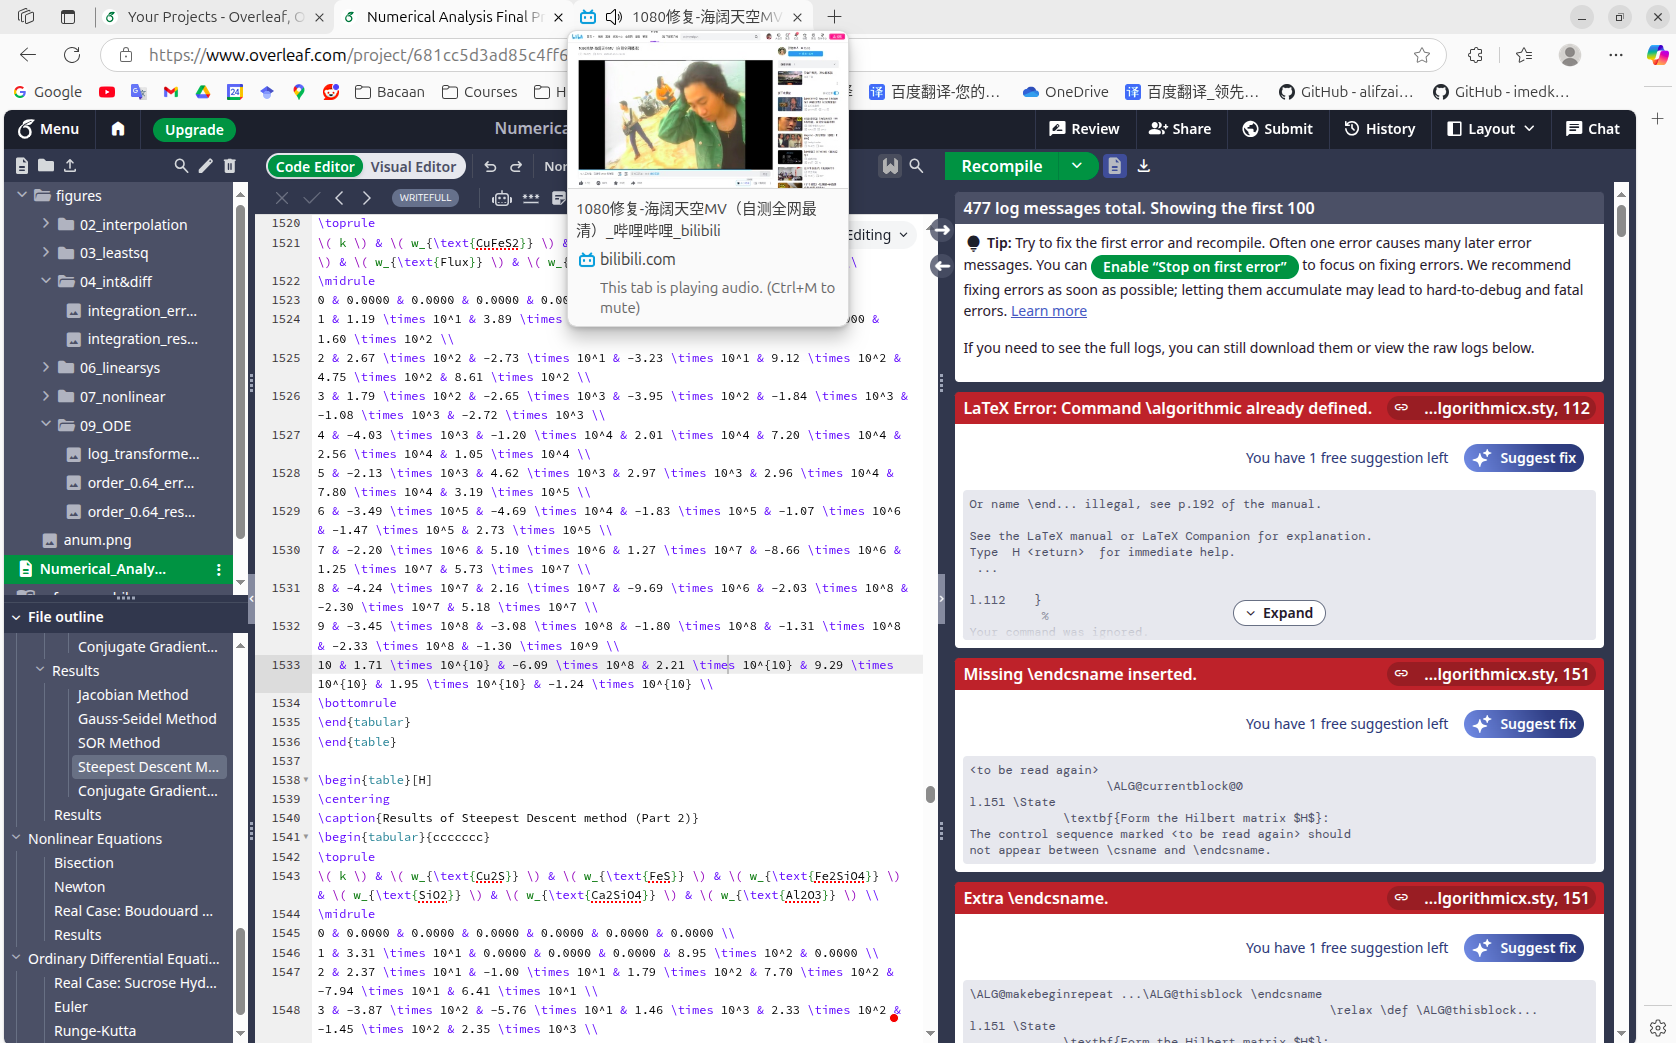
\includegraphics[width=\linewidth]{figures/06_linearsys/Screenshot from 2025-05-18 19-57-18.png}
    \caption{Unable to compile due to large number}
    \label{fig:enter-label}
\end{figure}

\begin{figure}[H]
    \centering
    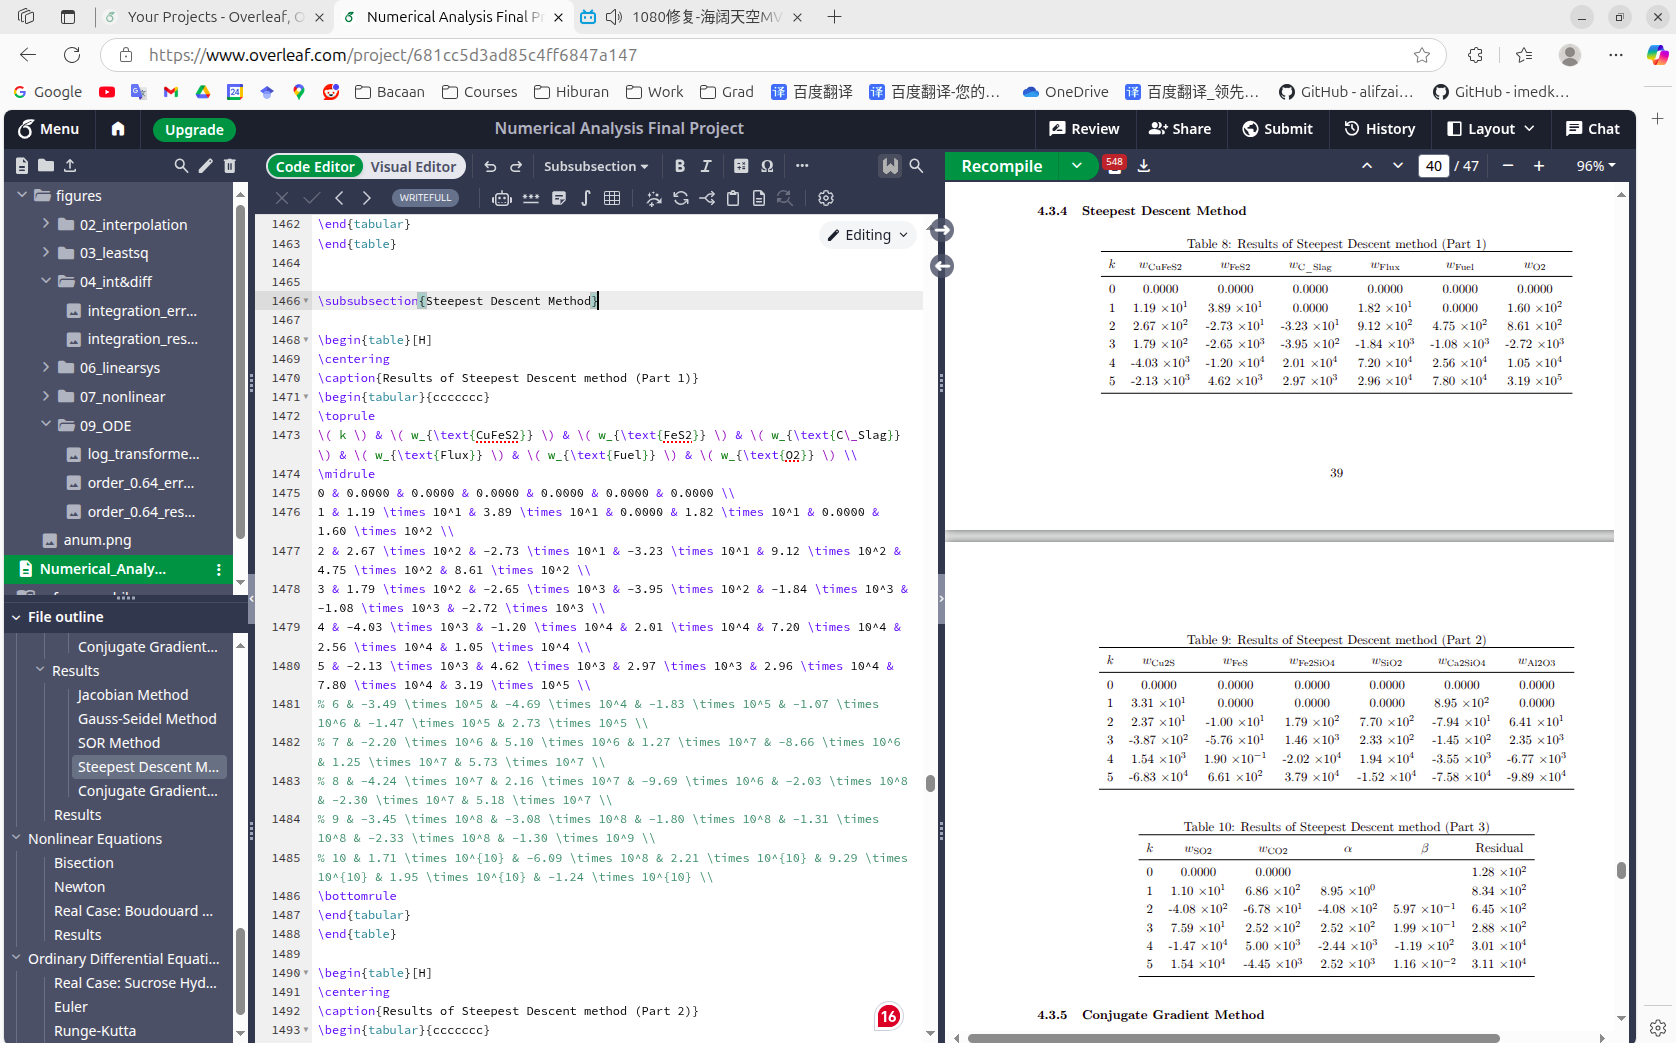
\includegraphics[width=\linewidth]{figures/06_linearsys/Screenshot from 2025-05-18 19-59-09.png}
    \caption{Only show half of max iteration :(}
    \label{fig:enter-label}
\end{figure}




\subsubsection{Conjugate Gradient Method}


\begin{table}[H]
\centering
\caption{Results of Conjugate Gradient method (Part 1)}
\begin{tabular}{cccccccc}
\toprule
\( k \) & \( w_{\text{CuFeS2}} \) & \( w_{\text{FeS2}} \) & \( w_{\text{C\_Slag}} \) & \( w_{\text{Flux}} \) & \( w_{\text{Fuel}} \) & \( w_{\text{O2}} \) & \( w_{\text{N2}} \) \\
\midrule
0 & 0.0000 & 0.0000 & 0.0000 & 0.0000 & 0.0000 & 0.0000 & 0.0000 \\
1 & 11.8534 & 38.8883 & 0.0000 & 18.2230 & 0.0000 & 160.1691 & 37.0633 \\
2 & 26.4679 & -31.0606 & -4.2131 & 106.0731 & 62.0286 & -0.8353 & 170.2829 \\
3 & 39.1477 & 16.3453 & -2.1001 & 148.9784 & 77.9697 & 156.0524 & 198.8193 \\
4 & -214.4401 & -7050.3375 & -1873.1774 & -9624.0332 & -4274.7193 & -14682.9149 & 4999.7204 \\
5 & 363.5734 & 7269.9871 & 1848.1179 & 10119.7885 & 4540.7178 & 15419.3319 & -4452.4879 \\
6 & 95.7469 & -157.5146 & -116.9182 & -150.8443 & -33.9928 & -175.9652 & 587.9656 \\
7 & 130.9044 & 63.2694 & -93.9381 & 120.4240 & 93.1006 & 237.1970 & 557.1989 \\
8 & 311.5840 & 1977.9058 & 165.9106 & 2580.0815 & 1194.4393 & 3198.6350 & 8.6722 \\
9 & -179.4649 & -4390.7281 & -797.0186 & -5750.2975 & -2519.0523 & -6619.1756 & 2130.9367 \\
10 & 342.5440 & 1710.9291 & 78.3454 & 2158.3552 & 1012.5862 & 2784.3617 & 236.2954 \\
\bottomrule
\end{tabular}
\end{table}

\begin{table}[H]
\centering
\caption{Results of Conjugate Gradient method (Part 2)}
\begin{tabular}{cccccccc}
\toprule
\( k \) & \( w_{\text{Cu2S}} \) & \( w_{\text{FeS}} \) & \( w_{\text{Fe2SiO4}} \) & \( w_{\text{SiO2}} \) & \( w_{\text{Ca2SiO4}} \) & \( w_{\text{Al2O3}} \) & \( w_{\text{Cu2O}} \) \\
\midrule
0 & 0.0000 & 0.0000 & 0.0000 & 0.0000 & 0.0000 & 0.0000 & 0.0000 \\
1 & 33.1360 & 0.0000 & 0.0000 & 0.0000 & 8.95 \times 10^2 & 0.0000 & 8.95 \times 10^1 \\
2 & -20.3315 & -1.3067 & 2.34 \times 10^1 & -5.32 \times 10^2 & -1.04 \times 10^1 & -5.49 \times 10^1 & -6.78 \times 10^1 \\
3 & 8.1490 & -1.0944 & 1.58 \times 10^2 & 1.58 \times 10^2 & -1.34 \times 10^1 & 1.59 \times 10^1 & -1.42 \times 10^1 \\
4 & -2436.7036 & -118.6226 & -2.14 \times 10^3 & -7.05 \times 10^3 & -1.87 \times 10^3 & -9.62 \times 10^3 & -4.27 \times 10^3 \\
5 & 2519.1301 & 116.9826 & 3.64 \times 10^2 & 7.27 \times 10^3 & 1.85 \times 10^3 & 1.01 \times 10^4 & 4.54 \times 10^3 \\
6 & -50.6906 & -6.4989 & 9.57 \times 10^1 & -1.58 \times 10^2 & -1.17 \times 10^2 & -1.51 \times 10^2 & -3.40 \times 10^1 \\
7 & 32.0940 & -3.7953 & 1.31 \times 10^2 & 6.33 \times 10^1 & -9.39 \times 10^1 & 1.20 \times 10^2 & 9.31 \times 10^1 \\
8 & 823.9719 & 26.8669 & 3.12 \times 10^2 & 1.98 \times 10^3 & 1.66 \times 10^2 & 2.58 \times 10^3 & 1.19 \times 10^3 \\
9 & -1817.3784 & -80.2385 & -1.79 \times 10^2 & -4.39 \times 10^3 & -7.97 \times 10^2 & -5.75 \times 10^3 & -2.52 \times 10^3 \\
10 & 712.1424 & 20.0331 & 3.43 \times 10^2 & 1.71 \times 10^3 & 7.83 \times 10^1 & 2.16 \times 10^3 & 1.01 \times 10^3 \\
\bottomrule
\end{tabular}
\end{table}


\begin{table}[H]
\centering
\caption{Results of Conjugate Gradient method (Part 3)}
\begin{tabular}{cccccccc}
\toprule
\( k \) & \( w_{\text{SO2}} \) & \( w_{\text{CO2}} \) & \( \alpha \) & \( \beta \) & Residual \\
\midrule
0 & 0.0000 & 0.0000 &  &  & 127.8830 \\
1 & 1.10 \times 10^1 & 6.86 \times 10^2 & 8.95 \times 10^0 &  & 834.2690 \\
2 & -4.08 \times 10^2 & -6.78 \times 10^1 & -4.08 \times 10^2 & 0.5970 & 644.5874 \\
3 & 7.59 \times 10^1 & 0.2580 & 0.2580 & 0.1991 & 287.5950 \\
4 & -1.47 \times 10^4 & 5.00 \times 10^3 & -2.44 \times 10^3 & -1.19 \times 10^2 & 30098.1827 \\
5 & 1.54 \times 10^4 & -4.45 \times 10^3 & 2.52 \times 10^3 & 0.0116 & 31142.3866 \\
6 & -1.76 \times 10^2 & 5.88 \times 10^2 & -5.07 \times 10^1 & -0.0056 & 801.7977 \\
7 & 5.57 \times 10^2 & 3.21 \times 10^1 & 3.21 \times 10^1 & 0.2083 & 717.6400 \\
8 & 8.67 \times 10^0 & 1.83 \times 10^1 & 1.83 \times 10^1 & 1.82 \times 10^1 & 6810.7401 \\
9 & 2.13 \times 10^3 & -1.82 \times 10^3 & -1.82 \times 10^3 & -0.0672 & 14524.4245 \\
10 & 2.36 \times 10^2 & 0.0142 & 0.0142 & 0.1699 & 5987.2638 \\
\bottomrule
\end{tabular}
\end{table}



\subsection{Comparison}
\begin{figure}[H]
    \centering
    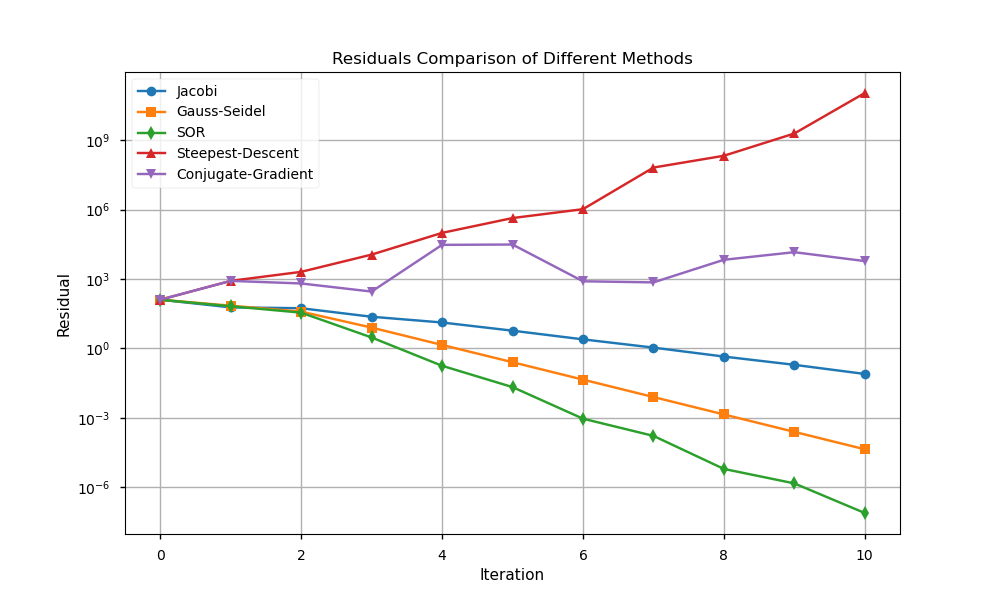
\includegraphics[width=\imagewidth\textwidth]{figures/06_linearsys/residuals_comparison.png}
    \caption{Residual comparison from different method}
\end{figure}


\section{Nonlinear Equations}
\subsection{Real Case: Boudouard Reaction Equilibrium}

The Boudouard reaction is a chemical equilibrium reaction that describes the conversion of carbon monoxide (\(\text{CO}\)) to carbon dioxide (\(\text{CO}_2\)) and solid carbon (C) at high temperatures. The reaction is represented as:
\begin{equation}
2 \text{CO} \leftrightarrow \text{CO}_2 + \text{C}
\end{equation}

This reaction is important in various industrial processes, such as the production of synthesis gas and the reduction of iron ore.

Given the fraction of CO (\( x_{\text{CO}} \)) in the gas mixture, the equilibrium constant \( K \) for the Boudouard reaction can be expressed as:
\begin{equation}
K = \frac{P_{\text{CO}_2} \cdot P_{\text{C}}}{P_{\text{CO}}^2}
\end{equation}

Where:
\begin{itemize}
    \item \( P_{\text{CO}} \) is the partial pressure of \(\text{CO}\).
    \item \( P_{\text{CO}_2} \) is the partial pressure of \(\text{CO}_2\).
    \item \( P_{\text{C}} \) is the partial pressure of solid carbon (which is often considered to be 1 atm).
\end{itemize}

Given \( x_{\text{CO}} = \frac{n_{\text{CO}}}{n_{\text{CO}} + n_{\text{CO}_2}} \), we can express the partial pressures in terms of \( x_{\text{CO}} \):
\begin{equation}
P_{\text{CO}} = x_{\text{CO}} \cdot P_{\text{total}}
\end{equation}
\begin{equation}
P_{\text{CO}_2} = (1 - x_{\text{CO}}) \cdot P_{\text{total}}
\end{equation}

Assuming \( P_{\text{total}} = 1 \) atm for simplicity, the equilibrium constant \( K \) becomes:
\begin{equation}
K = \frac{(1 - x_{\text{CO}})}{x_{\text{CO}}^2}
\end{equation}

Taking the natural logarithm of both sides:
\begin{equation}
\ln K = \ln \left( \frac{1 - x_{\text{CO}}}{x_{\text{CO}}^2} \right)
\end{equation}

The Gibbs free energy change (\( \Delta G \)) for the reaction can be related to the equilibrium constant \( K \) by:
\begin{equation}
\Delta G = -RT \ln K
\end{equation}

Where:
\begin{itemize}
    \item \( R \) is the universal gas constant.
    \item \( T \) is the temperature in Kelvin.
\end{itemize}

The enthalpy change (\( \Delta H \)) and entropy change (\( \Delta S \)) for the reaction can be calculated using the Shomate equation parameters. The function \( f(T) \) representing the equilibrium condition is:
\begin{equation}
f(T) = \ln K + \frac{\Delta H(T)}{RT} - \frac{\Delta S(T)}{R}
\end{equation}

The Shomate parameters for \(\text{CO}\), \(\text{CO}_2\), and \(\text{C}_(s)\) are given as follows:
\begin{equation}
\begin{aligned}
\text{CO:} & \quad A_1 = 25.56759, \quad B_1 = 6.096130, \quad C_1 = 4.054656, \quad D_1 = -2.671301, \quad E_1 = 0.131021 \\
\text{\(\text{CO}_2\):} & \quad A_2 = 24.99735, \quad B_2 = 55.18696, \quad C_2 = -33.69137, \quad D_2 = 7.948387, \quad E_2 = -0.136638 \\
\text{C(s):} & \quad A_3 = 17.7289, \quad B_3 = 28.0988, \quad C_3 = -4.21434, \quad D_3 = 0.218050, \quad E_3 = -0.000281 \\
\end{aligned}
\end{equation}

The \(\Delta\) parameters for the reaction \( 2\text{CO} \rightarrow \text{CO}_2 + \text{C} \) are calculated as:
\begin{equation}
\begin{aligned}
\Delta A &= A_2 + A_3 - 2A_1 \\
\Delta B &= B_2 + B_3 - 2B_1 \\
\Delta C &= C_2 + C_3 - 2C_1 \\
\Delta D &= D_2 + D_3 - 2D_1 \\
\Delta E &= E_2 + E_3 - 2E_1 \\
\end{aligned}
\end{equation}

The enthalpy change (\( \Delta H \)) and entropy change (\( \Delta S \)) as functions of temperature are given by:
\begin{equation}
\begin{aligned}
\Delta H(T) &= \Delta H_{298} + \Delta A (T - 298) + \frac{\Delta B}{1000} \left( \frac{T^2}{2} - \frac{298^2}{2} \right) + \frac{\Delta C}{10^6} \left( \frac{T^3}{3} - \frac{298^3}{3} \right) \\
&\quad + \frac{\Delta D}{10^9} \left( \frac{T^4}{4} - \frac{298^4}{4} \right) + \Delta E \times 10^6 \left( -\frac{1}{T} + \frac{1}{298} \right) \\
\end{aligned}
\end{equation}

\begin{equation}
\begin{aligned}
\Delta S(T) &= \Delta S_{298} + \Delta A \ln \left( \frac{T}{298} \right) + \frac{\Delta B}{1000} (T - 298) + \frac{\Delta C}{2 \times 10^6} (T^2 - 298^2) \\
&\quad + \frac{\Delta D}{3 \times 10^9} (T^3 - 298^3) + \Delta E \times 10^6 \left( -\frac{1}{2T^2} + \frac{1}{2 \times 298^2} \right) \\
\end{aligned}
\end{equation}

Where:
\begin{itemize}
    \item \( \Delta H_{298} = -172459 \) J/mol
    \item \( \Delta S_{298} = -175.79 \) J/(mol K)
    \item \( R = 8.314 \) J/(mol K)
\end{itemize}

\newpage
\subsection{Method}
\subsubsection{Bisection}
The Bisection method is a root-finding method that repeatedly bisects an interval and then selects a subinterval in which a root must lie for further processing. The algorithm is as follows:

\begin{algorithm}[H]
\caption{Bisection Method}
\begin{algorithmic}[1]
\Require Function \( f \), interval \([a, b]\), maximum iterations \( \text{max\_iter} \)
\Ensure Approximation of the root of \( f(x) = 0 \)
\State Ensure \( f(a) \cdot f(b) < 0 \) (i.e., \( f \) changes sign over \([a, b]\))
\State Initialize \( \text{error} \gets b - a \)
\For{\( n = 1 \) to \( \text{max\_iter} \)}
    \State Compute the midpoint \( c \gets \frac{a + b}{2} \)
    \State Evaluate \( f(c) \)
    \State Update the error \( \text{error} \gets b - a \)
    \If{\( f(a) \cdot f(c) < 0 \)}
        \State \( b \gets c \)
    \Else
        \State \( a \gets c \)
    \EndIf
\EndFor
\State \textbf{return} \( c \) as the best approximation
\end{algorithmic}
\end{algorithm}

Python snippet for the bisection method:
\begin{lstlisting}[style=custompython][caption={Bisection method}, label=code:bs]
def bisection(x_CO, T_low=600, T_high=1200, max_iter=100):
    iterations = []
    for n in range(max_iter):
        T_mid = (T_low + T_high) / 2
        F_mid = f(T_mid, x_CO)
        F_low = f(T_low, x_CO)
        error = T_high - T_low
        iterations.append([n, T_mid, F_mid, error])
        if F_mid * F_low < 0:
            T_high = T_mid
        else:
            T_low = T_mid
    return pd.DataFrame(iterations, columns=["Iteration", "T", "f(T)", "Error"])
\end{lstlisting}

\subsubsection{Newton}
The Newton-Raphson method is an iterative root-finding algorithm that uses the first derivative of the function to approximate the root. The algorithm is as follows:
\begin{algorithm}[H]
\caption{Newton Method}
\begin{algorithmic}[1]
\Require Function \( f \), initial guess \( x_0 \), maximum iterations \( \text{max\_iter} \)
\Ensure Approximation of the root of \( f(x) = 0 \)
\State Initialize \( x \gets x_0 \)
\For{\( n = 1 \) to \( \text{max\_iter} \)}
    \State Compute \( f(x) \) and its derivative \( f'(x) \)
    \State Update the guess \( x_{\text{new}} \gets x - \frac{f(x)}{f'(x)} \)
    \State Compute the error \( \text{error} \gets |x_{\text{new}} - x| \)
    \State Update \( x \gets x_{\text{new}} \)
\EndFor
\State \textbf{return} \( x \) as the best approximation
\end{algorithmic}
\end{algorithm}

Python snippet for the newton method:
\begin{lstlisting}[style=custompython][caption={Newton method}, label=code:nt]
def newton_raphson(x_CO, T_guess=800, tol=1e-6, max_iter=100):
    T = T_guess
    iterations = []
    for n in range(max_iter):
        F = f(T, x_CO)
        dT = 1e-3
        F_plus = f(T + dT, x_CO)
        dFdT = (F_plus - F) / dT
        T_new = T - F / dFdT
        error = abs(T_new - T)
        iterations.append([n, T, F, error])
        # if error < tol:
        #     break
        T = T_new
    return pd.DataFrame(iterations, columns=["Iteration", "T", "f(T)", "Error"])
\end{lstlisting}


\subsection{Python Snippet for various method}
\begin{lstlisting}[style=custompython][caption={Comparison between Bisection and Newton method}, label=code:bsnt]
\begin{lstlisting}[style=custompython]
import numpy as np
import pandas as pd
import matplotlib.pyplot as plt
import os

# Shomate parameters (CO, CO₂, C(s))
A1, B1, C1, D1, E1 = 25.56759, 6.096130, 4.054656, -2.671301, 0.131021    # CO
A2, B2, C2, D2, E2 = 24.99735, 55.18696, -33.69137, 7.948387, -0.136638   # CO₂
A3, B3, C3, D3, E3 = 17.7289, 28.0988, -4.21434, 0.218050, -0.000281      # C(s)

# Δ parameters for 2CO → CO₂ + C
delta_A = A2 + A3 - 2*A1
delta_B = B2 + B3 - 2*B1
delta_C = C2 + C3 - 2*C1
delta_D = D2 + D3 - 2*D1
delta_E = E2 + E3 - 2*E1

# Standard values
delta_H_298 = -172459  # J/mol
delta_S_298 = -175.79  # J/(mol·K)
R = 8.314

# Functions for enthalpy and entropy changes
def delta_H(T):
    term1 = delta_A * (T - 298)
    term2 = (delta_B / 1000) * (T**2 / 2 - 298**2 / 2)
    term3 = (delta_C / 1e6) * (T**3 / 3 - 298**3 / 3)
    term4 = (delta_D / 1e9) * (T**4 / 4 - 298**4 / 4)
    term5 = delta_E * 1e6 * (-1/T + 1/298)
    return delta_H_298 + term1 + term2 + term3 + term4 + term5

def delta_S(T):
    term1 = delta_A * np.log(T / 298)
    term2 = (delta_B / 1000) * (T - 298)
    term3 = (delta_C / 2e6) * (T**2 - 298**2)
    term4 = (delta_D / 3e9) * (T**3 - 298**3)
    term5 = delta_E * 1e6 * (-1/(2*T**2) + 1/(2*298**2))
    return delta_S_298 + term1 + term2 + term3 + term4 + term5

# Equilibrium function
def f(T, x_CO):
    K = (1 - x_CO) / (x_CO**2)
    lnK = np.log(K)
    dH = delta_H(T)
    dS = delta_S(T)
    return lnK + dH/(R*T) - dS/R

# Newton-Raphson Solver
def newton_raphson(x_CO, T_guess=800, tol=1e-6, max_iter=100):
    T = T_guess
    iterations = []
    for n in range(max_iter):
        F = f(T, x_CO)
        dT = 1e-3
        F_plus = f(T + dT, x_CO)
        dFdT = (F_plus - F) / dT
        T_new = T - F / dFdT
        error = abs(T_new - T)
        iterations.append([n, T, F, error])
        T = T_new
    return pd.DataFrame(iterations, columns=["Iteration", "T", "f(T)", "Error"])

# Bisection Solver
def bisection(x_CO, T_low=600, T_high=1200, max_iter=100):
    iterations = []
    for n in range(max_iter):
        T_mid = (T_low + T_high) / 2
        F_mid = f(T_mid, x_CO)
        F_low = f(T_low, x_CO)
        error = T_high - T_low
        iterations.append([n, T_mid, F_mid, error])
        if F_mid * F_low < 0:
            T_high = T_mid
        else:
            T_low = T_mid
    return pd.DataFrame(iterations, columns=["Iteration", "T", "f(T)", "Error"])

# Solve for different x_CO values
x_CO_values = [0.1, 0.3, 0.5, 0.7, 0.9]
results_dir = "07_nonlinear/results"
os.makedirs(results_dir, exist_ok=True)

# Generate and save results
for x_CO in x_CO_values:
    df_nr = newton_raphson(x_CO, max_iter=20)
    df_bs = bisection(x_CO, max_iter=20)
    with pd.ExcelWriter(f"{results_dir}/xCO_{x_CO:.1f}_results.xlsx") as writer:
        df_nr.to_excel(writer, sheet_name="Newton-Raphson", index=False)
        df_bs.to_excel(writer, sheet_name="Bisection", index=False)

# Plot x_CO vs. T
plt.figure(figsize=(8, 5))
x_plot = x_CO_values
T_plot_nr = [newton_raphson(x, max_iter=20).iloc[-1]["T"] for x in x_plot]
plt.plot(x_plot, T_plot_nr, 'r-', marker='o', label="Newton")
plt.xlabel(r"$x_{\mathrm{CO}}$ = CO/(CO+CO₂)")
plt.ylabel("Temperature (K)")
plt.title("Boudouard Reaction Equilibrium")
plt.grid(True)
plt.savefig(f"{results_dir}/xCO_vs_T.png")
plt.close()

# Plot error convergence for Newton-Raphson
plt.figure(figsize=(10, 6))
markerss = ['o', 's', 'd', '^', 'v', 'p', '*', 'h', '+', 'x']
for i, x_CO in enumerate(x_CO_values):
    df = pd.read_excel(f"{results_dir}/xCO_{x_CO:.1f}_results.xlsx", sheet_name="Newton-Raphson")
    plt.semilogy(df["Iteration"], df["Error"], marker=markerss[i], label=f"$x_{{\\mathrm{{CO}}}}$ = {x_CO}")
plt.xlabel("Iteration")
plt.ylabel("Error (log scale)")
plt.title("Newton Error Convergence")
plt.grid(True, which="both", ls="--")
plt.legend()
plt.tight_layout()
plt.savefig(f"{results_dir}/newton_error_convergence.png")
plt.close()

# Plot error convergence for Bisection
plt.figure(figsize=(10, 6))
for i, x_CO in enumerate(x_CO_values):
    df = pd.read_excel(f"{results_dir}/xCO_{x_CO:.1f}_results.xlsx", sheet_name="Bisection")
    plt.semilogy(df["Iteration"], df["Error"], marker=markerss[i], label=f"$x_{{\\mathrm{{CO}}}}$ = {x_CO}")
plt.xlabel("Iteration")
plt.ylabel("Error (log scale)")
plt.title("Bisection Error Convergence")
plt.grid(True, which="both", ls="--")
plt.legend()
plt.tight_layout()
plt.savefig(f"{results_dir}/bisection_error_convergence.png")
plt.close()

# Plot value convergence for Newton-Raphson
plt.figure(figsize=(10, 6))
for i, x_CO in enumerate(x_CO_values):
    df = pd.read_excel(f"{results_dir}/xCO_{x_CO:.1f}_results.xlsx", sheet_name="Newton-Raphson")
    plt.plot(df["Iteration"], df["T"], marker=markerss[i], label=f"T at $x_{{\\mathrm{{CO}}}}$ = {x_CO}")
plt.xlabel("Iteration")
plt.ylabel("T (K)")
plt.title("Newton Temperature Convergence")
plt.grid(True, which="both", ls="--")
plt.legend()
plt.tight_layout()
plt.savefig(f"{results_dir}/Newton_Temperature_convergence.png")
plt.close()

# Plot value convergence for Bisection
plt.figure(figsize=(10, 6))
for i, x_CO in enumerate(x_CO_values):
    df = pd.read_excel(f"{results_dir}/xCO_{x_CO:.1f}_results.xlsx", sheet_name="Bisection")
    plt.plot(df["Iteration"], df["T"], marker=markerss[i], label=f"T at $x_{{\\mathrm{{CO}}}}$ = {x_CO}")
plt.xlabel("Iteration")
plt.ylabel("T (K)")
plt.title("Bisection Temperature Convergence")
plt.grid(True, which="both", ls="--")
plt.legend()
plt.tight_layout()
plt.savefig(f"{results_dir}/Bisection_Temperature_convergence.png")
plt.close()

\end{lstlisting}


\newpage
\subsection{Results}
\subsubsection{Bisection}


\begin{table}[H]
\centering
\caption{Bisection Method Results for Different \( x_{\text{CO}} \) Values}
\begin{tabular}{cccccccccc}
\toprule
Iteration & \multicolumn{3}{c}{\( x_{\text{CO}} = 0.3 \)} & \multicolumn{3}{c}{\( x_{\text{CO}} = 0.5 \)} & \multicolumn{3}{c}{\( x_{\text{CO}} = 0.7 \)} \\
% \cmidrule(r){2-4} \cmidrule(r){5-7} \cmidrule(r){8-10}
\cmidrule(r){2-10}
 & \( T \) & \( f(T) \) & Error & \( T \) & \( f(T) \) & Error & \( T \) & \( f(T) \) & Error \\
\midrule
0 & 900 & -0.54 & 600 & 900 & -1.90 & 600 & 900 & -3.09 & 600 \\
1 & 1050 & 2.50 & 300 & 1050 & 1.14 & 300 & 1050 & -0.04 & 300 \\
2 & 975 & 1.10 & 150 & 975 & -0.25 & 150 & 1125 & 1.15 & 150 \\
3 & 937.50 & 0.32 & 75 & 1012.50 & 0.47 & 75 & 1087.50 & 0.57 & 75 \\
4 & 918.75 & -0.11 & 37.50 & 993.75 & 0.12 & 37.50 & 1068.75 & 0.27 & 37.50 \\
5 & 928.13 & 0.11 & 18.75 & 984.38 & -0.07 & 18.75 & 1059.38 & 0.11 & 18.75 \\
6 & 923.44 & 0.00 & 9.38 & 989.06 & 0.02 & 9.38 & 1054.69 & 0.04 & 9.38 \\
7 & 921.09 & -0.05 & 4.69 & 986.72 & -0.02 & 4.69 & 1052.34 & 0.00 & 4.69 \\
8 & 922.27 & -0.02 & 2.34 & 987.89 & 0.00 & 2.34 & 1053.52 & 0.02 & 2.34 \\
9 & 922.85 & -0.01 & 1.17 & 987.30 & -0.01 & 1.17 & 1052.93 & 0.01 & 1.17 \\
10 & 923.14 & 0.00 & 0.59 & 987.60 & 0.00 & 0.59 & 1052.64 & 0.00 & 0.59 \\
11 & 923.29 & 0.00 & 0.29 & 987.74 & 0.00 & 0.29 & 1052.49 & 0.00 & 0.29 \\
12 & 923.36 & 0.00 & 0.15 & 987.82 & 0.00 & 0.15 & 1052.56 & 0.00 & 0.15 \\
13 & 923.33 & 0.00 & 0.07 & 987.78 & 0.00 & 0.07 & 1052.60 & 0.00 & 0.07 \\
14 & 923.35 & 0.00 & 0.04 & 987.80 & 0.00 & 0.04 & 1052.62 & 0.00 & 0.04 \\
15 & 923.36 & 0.00 & 0.02 & 987.81 & 0.00 & 0.02 & 1052.61 & 0.00 & 0.02 \\
16 & 923.36 & 0.00 & 0.01 & 987.80 & 0.00 & 0.01 & 1052.61 & 0.00 & 0.01 \\
17 & 923.36 & 0.00 & 0.00 & 987.80 & 0.00 & 0.00 & 1052.61 & 0.00 & 0.00 \\
18 & 923.36 & 0.00 & 0.00 & 987.80 & 0.00 & 0.00 & 1052.61 & 0.00 & 0.00 \\
19 & 923.36 & 0.00 & 0.00 & 987.80 & 0.00 & 0.00 & 1052.61 & 0.00 & 0.00 \\
20 & 923.36 & 0.00 & 0.00 & 987.80 & 0.00 & 0.00 & 1052.61 & 0.00 & 0.00 \\
\bottomrule
\end{tabular}
\end{table}


\begin{figure}[H]
    \centering
    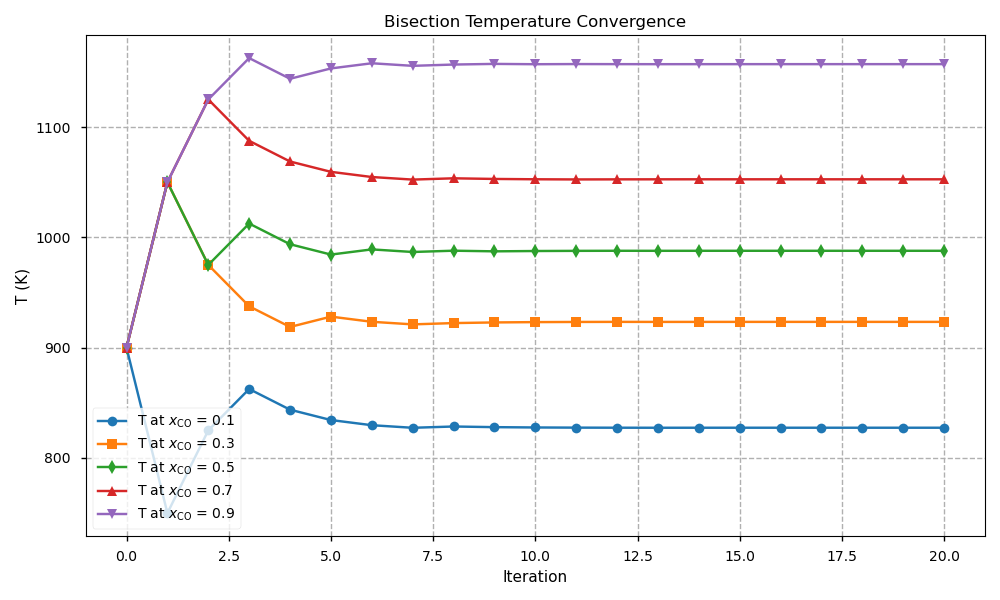
\includegraphics[width=\imagewidth\textwidth]{figures/07_nonlinear/Bisection_Temperature_convergence.png}
    \caption{Temperature convergence using bisection method}
\end{figure}
\begin{figure}[H]
    \centering
    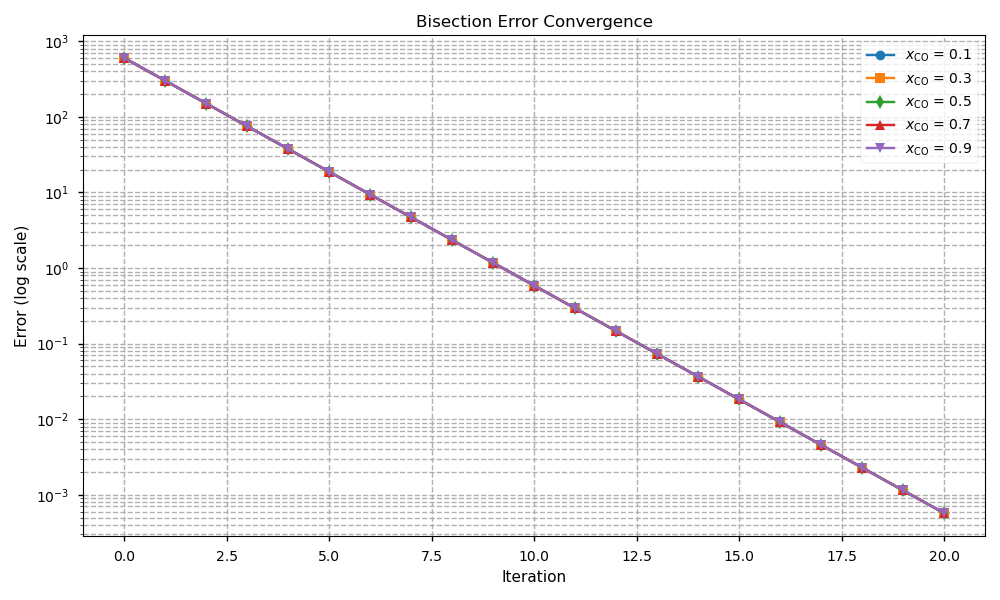
\includegraphics[width=\imagewidth\textwidth]{figures/07_nonlinear/bisection_error_convergence.png}
    \caption{Error from bisection method}
\end{figure}


\subsubsection{Newton}



\begin{table}[H]
\centering
\caption{Newton Method Results for Different \( x_{\text{CO}} \) Values}
\begin{tabular}{cccccccccc}
\toprule
Iteration & \multicolumn{3}{c}{\( x_{\text{CO}} = 0.3 \)} & \multicolumn{3}{c}{\( x_{\text{CO}} = 0.5 \)} & \multicolumn{3}{c}{\( x_{\text{CO}} = 0.7 \)} \\
\cmidrule(r){2-10}
 & \( T \) & \( f(T) \) & Error & \( T \) & \( f(T) \) & Error & \( T \) & \( f(T) \) & Error \\
\midrule
0 & 800 & -3.26 & 105.87 & 800 & -4.62 & 149.93 & 800 & -5.81 & 188.34 \\
1 & 905.87 & -0.40 & 17.13 & 949.93 & -0.77 & 36.29 & 988.34 & -1.17 & 59.99 \\
2 & 923.00 & -0.01 & 0.36 & 986.23 & -0.03 & 1.57 & 1048.33 & -0.07 & 4.26 \\
3 & 923.36 & 0.00 & 0.00 & 987.80 & 0.00 & 0.00 & 1052.59 & 0.00 & 0.02 \\
4 & 923.36 & 0.00 & 0.00 & 987.80 & 0.00 & 0.00 & 1052.61 & 0.00 & 0.00 \\
5 & 923.36 & 0.00 & 0.00 & 987.80 & 0.00 & 0.00 & 1052.61 & 0.00 & 0.00 \\
6 & 923.36 & 0.00 & 0.00 & 987.80 & 0.00 & 0.00 & 1052.61 & 0.00 & 0.00 \\
7 & 923.36 & 0.00 & 0.00 & 987.80 & 0.00 & 0.00 & 1052.61 & 0.00 & 0.00 \\
8 & 923.36 & 0.00 & 0.00 & 987.80 & 0.00 & 0.00 & 1052.61 & 0.00 & 0.00 \\
9 & 923.36 & 0.00 & 0.00 & 987.80 & 0.00 & 0.00 & 1052.61 & 0.00 & 0.00 \\
10 & 923.36 & 0.00 & 0.00 & 987.80 & 0.00 & 0.00 & 1052.61 & 0.00 & 0.00 \\
11 & 923.36 & 0.00 & 0.00 & 987.80 & 0.00 & 0.00 & 1052.61 & 0.00 & 0.00 \\
12 & 923.36 & 0.00 & 0.00 & 987.80 & 0.00 & 0.00 & 1052.61 & 0.00 & 0.00 \\
13 & 923.36 & 0.00 & 0.00 & 987.80 & 0.00 & 0.00 & 1052.61 & 0.00 & 0.00 \\
14 & 923.36 & 0.00 & 0.00 & 987.80 & 0.00 & 0.00 & 1052.61 & 0.00 & 0.00 \\
15 & 923.36 & 0.00 & 0.00 & 987.80 & 0.00 & 0.00 & 1052.61 & 0.00 & 0.00 \\
16 & 923.36 & 0.00 & 0.00 & 987.80 & 0.00 & 0.00 & 1052.61 & 0.00 & 0.00 \\
17 & 923.36 & 0.00 & 0.00 & 987.80 & 0.00 & 0.00 & 1052.61 & 0.00 & 0.00 \\
18 & 923.36 & 0.00 & 0.00 & 987.80 & 0.00 & 0.00 & 1052.61 & 0.00 & 0.00 \\
19 & 923.36 & 0.00 & 0.00 & 987.80 & 0.00 & 0.00 & 1052.61 & 0.00 & 0.00 \\
20 & 923.36 & 0.00 & 0.00 & 987.80 & 0.00 & 0.00 & 1052.61 & 0.00 & 0.00 \\
\bottomrule
\end{tabular}
\end{table}


\begin{figure}[H]
    \centering
    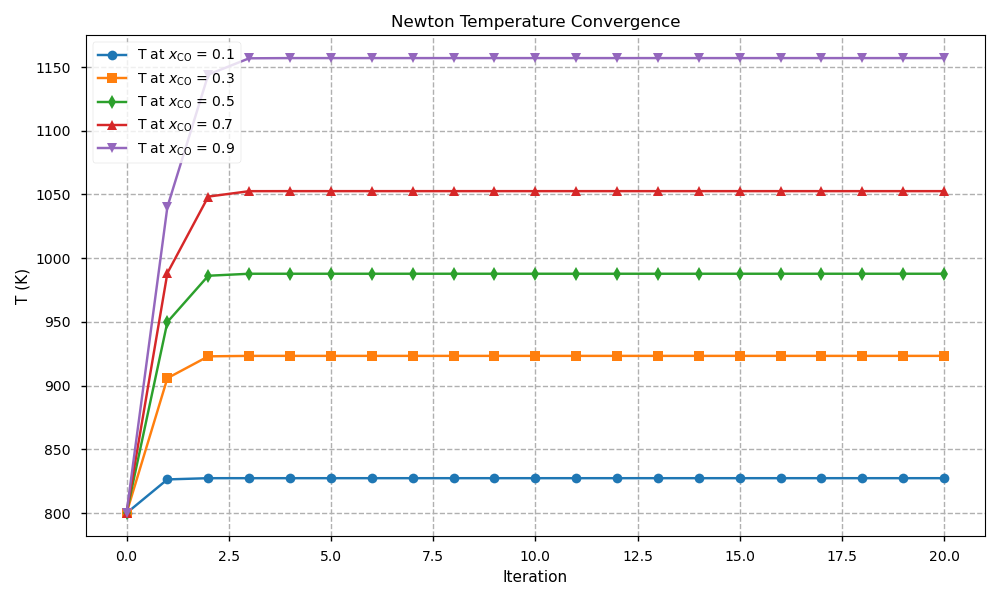
\includegraphics[width=\imagewidth\textwidth]{figures/07_nonlinear/Newton_Temperature_convergence.png}
    \caption{Temperature convergence using newton method}
\end{figure}

\begin{figure}[H]
    \centering
    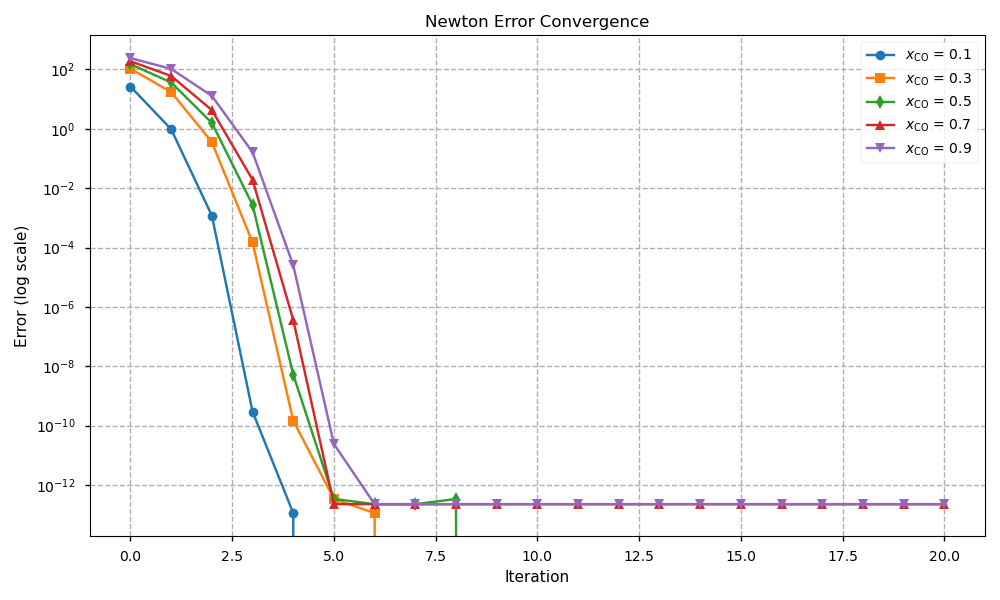
\includegraphics[width=\imagewidth\textwidth]{figures/07_nonlinear/newton_error_convergence.png}
    \caption{Error from newton method}
\end{figure}

\subsubsection{Boudouard Reaction}
\begin{figure}[H]
    \centering
    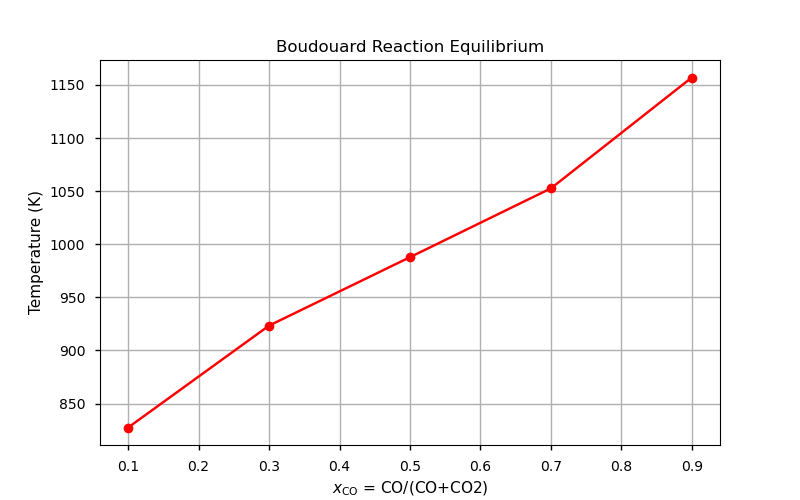
\includegraphics[width=\imagewidth\textwidth]{figures/07_nonlinear/xCO_vs_T.png}
    \caption{Boudouard Reaction from known CO fraction}
\end{figure}

\subsubsection{Key Observations}
\begin{itemize}
    \item The Bisection method is guaranteed to converge if the function changes sign over the interval. It is robust but can be slow.
    \item The Newton-Raphson method converges quickly if the initial guess is close to the root. However, it requires the derivative of the function and may not converge if the initial guess is not good.
\end{itemize}

\section{Ordinary Differential Equation}
\subsection{Real Case: Sucrose Hydrolysis Reaction Profile}
Reaction kinetics is the study of the rates of chemical reactions and the factors that influence these rates. For sucrose hydrolysis, the reaction rate is described by the rate equation above. The reaction order \( n \) indicates how the rate of reaction changes with the concentration of sucrose. For example:
\begin{itemize}
    \item If \( n = 1 \), the reaction is first-order, meaning the rate is directly proportional to the concentration of sucrose.
    \item If \( n = 2 \), the reaction is second-order, meaning the rate is proportional to the square of the concentration.
\end{itemize}
The reaction rate constant \( k \) is a proportionality constant that depends on factors such as temperature and the presence of a catalyst. It quantifies how quickly the reaction proceeds under given conditions.

Sucrose hydrolysis is an acid-catalyzed reaction governed by the rate equation:
\begin{equation}
    -\frac{dC_A}{dt} = k{C_A}^n
\end{equation}
where:
\begin{itemize}
    \item \( C_A \): Concentration of sucrose (reactant)
    \item \( k \): Reaction rate constant (depends on temperature and catalyst)
    \item \( n \): Reaction order (determines rate dependence on concentration)
\end{itemize}

The code calculates \( n \) and \( k \) using experimental data and logarithmic transformation:
\begin{equation}
    \ln(-\frac{dC_A}{dt}) = \ln(k) + n\ln(C_A)
\end{equation}
\begin{itemize}
    \item Numerical derivatives approximate \(\frac{dC_A}{dt}\)
    \item Least squares regression determines \( n \) (slope) and \( k = e^{\text{intercept}} \)
\end{itemize}
\begin{table}[H]
\centering
\caption{Experimental Data for Sucrose Hydrolysis}
\begin{tabular}{cc}
\toprule
\( t \) (hours) & \( C_A \) (mmol/liter) \\
\midrule
0 & 1.00 \\
1 & 0.84 \\
2 & 0.68 \\
3 & 0.53 \\
4 & 0.38 \\
5 & 0.27 \\
6 & 0.16 \\
7 & 0.09 \\
8 & 0.04 \\
9 & 0.018 \\
10 & 0.006 \\
11 & 0.0025 \\
\bottomrule
\end{tabular}
\end{table}

\subsection{Method}
\subsubsection{Euler}

\begin{algorithm}[H]
\caption{Euler Method}
\begin{algorithmic}[1]
\Require Initial time \( t_0 \), initial concentration \( C_{A0} \), step size \( h \), final time \( t_f \), ODE function \( f(t, C_A) \)
\Ensure Approximate concentration profile
\State Initialize \( C_A(t_0) = C_{A0} \)
\For{\( t = t_0 + h \) to \( t_f \) step \( h \)}
    \State \( C_A(t) = C_A(t - h) + h \cdot f(t - h, C_A(t - h)) \)
\EndFor
\end{algorithmic}
\end{algorithm}

Python snippet for the Euler method:
\begin{lstlisting}[style=custompython][caption={Euler method}, label=code:eu]
def euler(self) -> Tuple[np.ndarray, np.ndarray]:
        y = np.zeros(len(self.t))
        y[0] = self.y0
        for i in range(1, len(self.t)):
            y[i] = y[i-1] + self.h * self.f(self.t[i-1], y[i-1])
            
        return self.t, y
\end{lstlisting}


Key features:
\begin{itemize}
    \item First-order accuracy
    \item Simplest numerical integration method
    \item Prone to instability for stiff equations
\end{itemize}


\subsubsection{Runge-Kutta}
\begin{algorithm}[H]
\caption{4th Order Runge-Kutta Method}
\begin{algorithmic}[1]
\Require Same inputs as Euler method
\Ensure More accurate concentration profile
\For{\( t = t_0 + h \) to \( t_f \) step \( h \)}
    \State \( k_1 = f(t - h, C_A(t - h)) \)
    \State \( k_2 = f(t - \frac{h}{2}, C_A(t - h) + \frac{h}{2}k_1) \)
    \State \( k_3 = f(t - \frac{h}{2}, C_A(t - h) + \frac{h}{2}k_2) \)
    \State \( k_4 = f(t, C_A(t - h) + hk_3) \)
    \State \( C_A(t) = C_A(t - h) + \frac{h}{6}(k_1 + 2k_2 + 2k_3 + k_4) \)
\EndFor
\end{algorithmic}
\end{algorithm}

Python snippet for the Runge-Kutta 4 method:
\begin{lstlisting}[style=custompython][caption={Runge-Kutta 4 method}, label=code:rk4]
def runge_kutta4(self) -> Tuple[np.ndarray, np.ndarray]:
    y = np.zeros(len(self.t))
    y[0] = self.y0
    for i in range(1, len(self.t)):
        t_prev = self.t[i-1]
        y_prev = y[i-1]
        h = self.h
        k1 = self.f(t_prev, y_prev)
        k2 = self.f(t_prev + h/2, y_prev + h/2 * k1)
        k3 = self.f(t_prev + h/2, y_prev + h/2 * k2)
        k4 = self.f(t_prev + h, y_prev + h * k3)
        y[i] = y_prev + h/6 * (k1 + 2*k2 + 2*k3 + k4)
        
    return self.t, y
\end{lstlisting}

Key features:
\begin{itemize}
    \item Fourth-order accuracy
    \item Balances computational effort and precision
    \item Requires four function evaluations per step
\end{itemize}





\subsection{Python snippet for various method}

\begin{lstlisting}[style=custompython][caption={Comparing Euler and Runge-Kutta 4 method}, label=code:eurk4]
import numpy as np
import pandas as pd
import matplotlib.pyplot as plt
import os
from typing import Callable, Optional, Tuple

# Define ODE solver class
class ODESolver:
    def __init__(self, 
                 f: Callable[[float, float], float], 
                 y0: float, 
                 t0: float, 
                 tf: float, 
                 h: float,
                 primitive: Optional[Callable[[float], float]] = None):

        self.f = f
        self.y0 = y0
        self.t0 = t0
        self.tf = tf
        self.h = h
        self.primitive = primitive
        
        # Create time array
        self.t = np.arange(t0, tf + h, h)
        
    def euler(self) -> Tuple[np.ndarray, np.ndarray]:
        y = np.zeros(len(self.t))
        y[0] = self.y0
        
        for i in range(1, len(self.t)):
            y[i] = y[i-1] + self.h * self.f(self.t[i-1], y[i-1])
            
        return self.t, y
    
    def runge_kutta4(self) -> Tuple[np.ndarray, np.ndarray]:
        y = np.zeros(len(self.t))
        y[0] = self.y0
        
        for i in range(1, len(self.t)):
            t_prev = self.t[i-1]
            y_prev = y[i-1]
            h = self.h
            
            k1 = self.f(t_prev, y_prev)
            k2 = self.f(t_prev + h/2, y_prev + h/2 * k1)
            k3 = self.f(t_prev + h/2, y_prev + h/2 * k2)
            k4 = self.f(t_prev + h, y_prev + h * k3)
            
            y[i] = y_prev + h/6 * (k1 + 2*k2 + 2*k3 + k4)
            
        return self.t, y

# Experimental data
t_exp = np.array([0, 1, 2, 3, 4, 5, 6, 7, 8, 9, 10, 11])
CA_exp = np.array([1.0, 0.84, 0.68, 0.53, 0.38, 0.27, 0.16, 0.09, 0.04, 0.018, 0.006, 0.0025])

# Function to define the ODE for different reaction orders
def create_f(n: float, k: float) -> Callable[[float, float], float]:
    def f(t: float, CA: float) -> float:
        return -k * CA**n
    return f

# Least squares fit function
def least_squares_fit(x, y, n):
    G = np.zeros((n+1, n+1))
    b = np.zeros(n+1)
    for j in range(n+1):
        for k in range(n+1):
            G[j, k] = np.sum(x**(j + k))
        b[j] = np.sum(y * x**j)
    try:
        beta = np.linalg.solve(G, b)
    except np.linalg.LinAlgError:
        beta = np.linalg.pinv(G) @ b  # Fallback to pseudo-inverse
    return beta, G, b

# Calculate the derivative using finite differences
dCA_dt = np.zeros_like(CA_exp)
for i in range(1, len(CA_exp) - 1):
    dCA_dt[i] = (CA_exp[i+1] - CA_exp[i-1]) / (t_exp[i+1] - t_exp[i-1])
dCA_dt[0] = (CA_exp[1] - CA_exp[0]) / (t_exp[1] - t_exp[0])
dCA_dt[-1] = (CA_exp[-1] - CA_exp[-2]) / (t_exp[-1] - t_exp[-2])

# Avoid log of negative or zero values
valid_indices = CA_exp > 0
ln_CA = np.log(CA_exp[valid_indices])
ln_dCA_dt = np.log(-dCA_dt[valid_indices])

# Perform least squares fit for the linear equation ln(-dCA/dt) = ln(k) + n*ln(CA)
beta, G, b = least_squares_fit(ln_CA, ln_dCA_dt, 1)
n_estimate = beta[1]
k_estimate = np.exp(beta[0])

# Create directory for least squares data if it doesn't exist
os.makedirs('09_ODE/least_square_data', exist_ok=True)

# Save Gram matrix, right-hand side vector, and least squares results to Excel
with pd.ExcelWriter('09_ODE/least_square_data/least_squares_results.xlsx') as writer:
    pd.DataFrame({'ln_CA': ln_CA, 'ln_dCA_dt': ln_dCA_dt}).to_excel(writer, sheet_name='Data', index=False)
    pd.DataFrame(G, columns=[f'G_{i}' for i in range(G.shape[1])]).to_excel(writer, sheet_name='Gram_Matrix', index=False)
    pd.DataFrame({'b': b}).to_excel(writer, sheet_name='RHS_Vector', index=False)
    pd.DataFrame({'beta': beta}).to_excel(writer, sheet_name='Results', index=False)

# Plot the log-transformed data
plt.figure(figsize=(10, 6))
plt.style.use('seaborn-v0_8-notebook')
plt.scatter(ln_CA, ln_dCA_dt, facecolors='none', edgecolors='black', linewidths=1, label='Experimental Data')
plt.plot(ln_CA, beta[0] + beta[1] * ln_CA, 'r-', label='Least Squares Fit')
plt.xlabel(r'$\ln(C_A)$')
plt.ylabel(r'$\ln(-dC_A/dt)$')
plt.title('Log-Transformed Rate Data')
plt.legend()
plt.grid(True)

# Create directory for plots if it doesn't exist
os.makedirs('09_ODE/plots', exist_ok=True)
plt.savefig('09_ODE/plots/log_transformed_rate_data.png')
plt.close()

# Function to find the best reaction order and constant
def find_best_order_and_constant():
    orders = [0.5, n_estimate, 0.7, 1.1]
    k_guess = k_estimate

    for n in orders:
        f = create_f(n, k_guess)
        solver = ODESolver(f, y0=1.0, t0=0, tf=11, h=1)
        df = solver.solve_and_compare()
        df['Experimental'] = CA_exp

        if 'Euler' in df.columns:
            df['Euler Error'] = np.abs(df['Euler'] - df['Experimental'])
        if 'Runge-Kutta4' in df.columns:
            df['RK4 Error'] = np.abs(df['Runge-Kutta4'] - df['Experimental'])

        print(f"Results for reaction order {n:0,.2f}:")
        print(df[['t', 'Euler', 'Runge-Kutta4', 'Experimental', 'Euler Error', 'RK4 Error']])
        print("\n")

        # Create directory for results if it doesn't exist
        os.makedirs('09_ODE/results', exist_ok=True)
        df.to_excel(f'09_ODE/results/order_{n:0,.2f}_results.xlsx', index=False)

        # Plot results for this reaction order
        plt.figure(figsize=(10, 6))
        plt.style.use('seaborn-v0_8-notebook')
        plt.scatter(df['t'], df['Experimental'], facecolors='none', edgecolors='black', linewidths=1, label='Experimental')
        plt.plot(df['t'], df['Euler'], 'b-', marker='o', label='Euler')
        plt.plot(df['t'], df['Runge-Kutta4'], 'r-', marker='s', label='Runge-Kutta 4')
        plt.xlabel('Time (hr)')
        plt.ylabel('Concentration (millimol/liter)')
        plt.title(f'Reaction Order {n:0,.2f}')
        plt.legend()
        plt.grid(True)
        plt.savefig(f'09_ODE/plots/order_{n:0,.2f}_results.png')
        plt.close()

# Run the analysis
find_best_order_and_constant()
\end{lstlisting}

\subsection{Results}

The estimated reaction order \( n \) and rate constant \( k \) are crucial for understanding the reaction mechanism and predicting the reaction profile. The results from the least squares regression provide the following estimates:
\begin{itemize}
    \item Estimated reaction order \( n \approx 0.64 \)
    \item Estimated rate constant \( k \approx 0.22 \)
\end{itemize}

These values indicate that the reaction is slightly more than first-order, suggesting that the rate of hydrolysis increases slightly faster than linearly with the concentration of sucrose. The rate constant \( k \) provides a measure of the reaction's speed under the given conditions.

\begin{figure}[H]
    \centering
    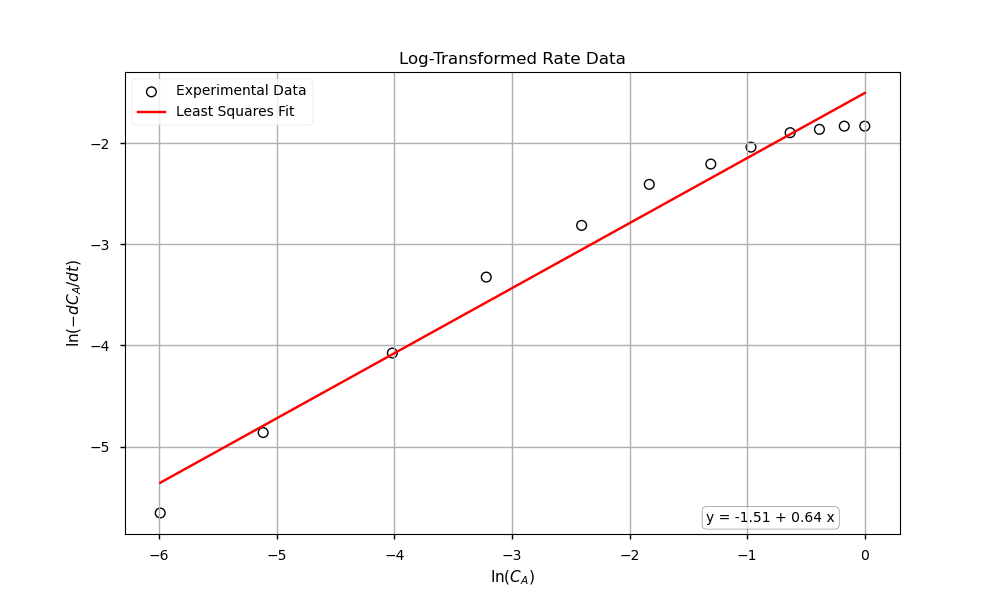
\includegraphics[width=\imagewidth\textwidth]{figures/09_ODE/log_transformed_rate_data.png}
    \caption{Interpolation data}
\end{figure}


The numerical solutions using Euler's method and the 4th order Runge-Kutta method were compared to the experimental data. The results are summarized in the following table:
\begin{table}[H]
\centering
\caption{Comparison of Numerical Methods for Sucrose Hydrolysis}
\begin{tabular}{cccccc}
\toprule
\( t \) & Euler & Runge-Kutta4 & Experimental & Euler Error & RK4 Error \\
\midrule
0 & 1.00 & 1.00 & 1.00 & 0.00 & 0.00 \\
1 & 0.78 & 0.79 & 0.84 & 0.06 & 0.05 \\
2 & 0.59 & 0.62 & 0.68 & 0.09 & 0.06 \\
3 & 0.43 & 0.47 & 0.53 & 0.10 & 0.06 \\
4 & 0.30 & 0.34 & 0.38 & 0.08 & 0.04 \\
5 & 0.20 & 0.24 & 0.27 & 0.07 & 0.03 \\
6 & 0.12 & 0.16 & 0.16 & 0.04 & 0.00 \\
7 & 0.06 & 0.10 & 0.09 & 0.03 & 0.01 \\
8 & 0.03 & 0.06 & 0.04 & 0.01 & 0.02 \\
9 & 0.00 & 0.03 & 0.02 & 0.01 & 0.01 \\
10 & 0.00 & 0.01 & 0.01 & 0.01 & 0.01 \\
11 &  & 0.00 & 0.00 &  & 0.00 \\
\bottomrule
\end{tabular}
\end{table}

\begin{figure}[H]
    \centering
    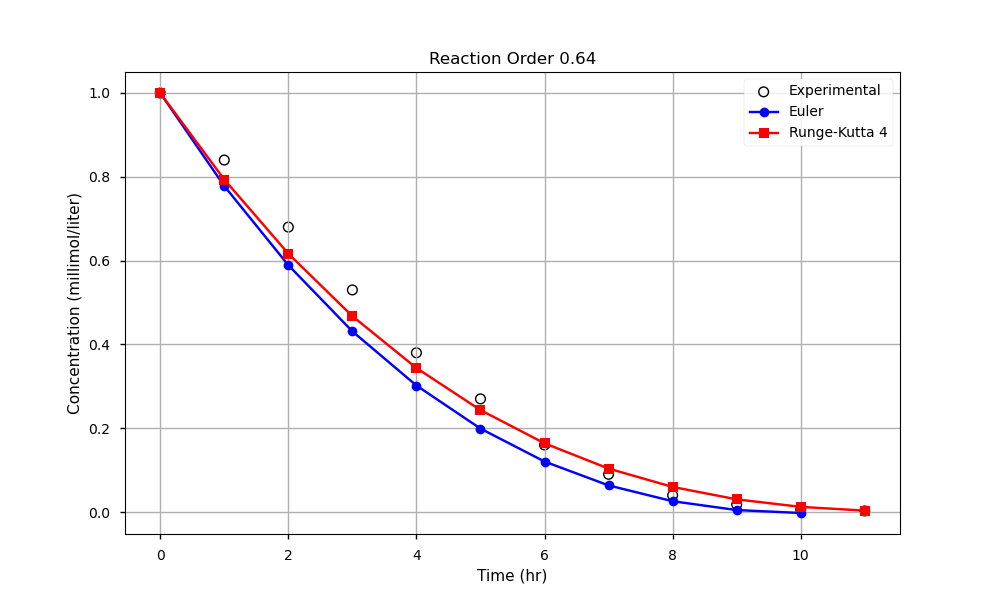
\includegraphics[width=\imagewidth\textwidth]{figures/09_ODE/order_0.64_results.png}
    \caption{Reaction profile result}
\end{figure}
\begin{figure}[H]
    \centering
    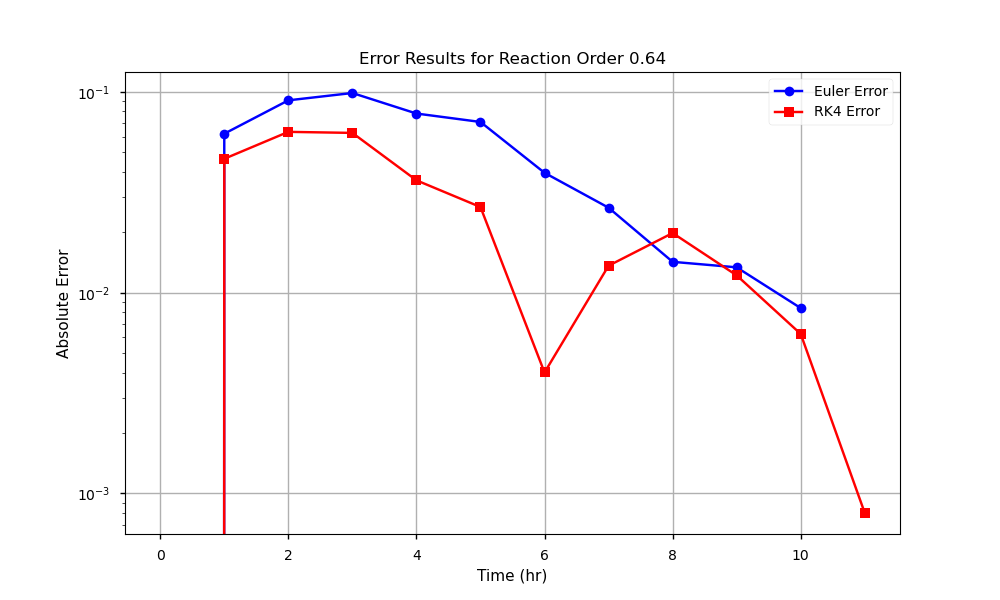
\includegraphics[width=\imagewidth\textwidth]{figures/09_ODE/order_0.64_errors.png}
    \caption{Error comparison}
\end{figure}


\subsection{Key Observations}
\begin{itemize}
    \item The estimated reaction order (\( n \)) determines the rate equation's nonlinearity
    \item Runge-Kutta 4 demonstrates superior accuracy compared to Euler method
    \item Experimental validation shows best match at \( n \approx 0.64 \)
    \item Error analysis highlights RK4's effectiveness in minimizing concentration prediction errors
    \item Numerical solutions must satisfy physical bounds (non-negative concentrations)
\end{itemize}













% \section{Special Case: Analysis of mass and energy balances in copper flash melting furnaces}

% \subsection{Introduction}

% Copper extraction has been a fundamental metallurgical process since antiquity, evolving from primitive smelting techniques to today's sophisticated pyrometallurgical methods\cite{davenport2002extractive}. Modern copper production predominantly relies on flash smelting technology, which accounts for over 50\% of global primary copper output\cite{schlesinger2011extractive}.

% Copper flash smelting has become the dominant production method since its development in the mid-20th century \cite{davenport2002extractive}. This process offers significant advantages over traditional methods, including higher energy efficiency \cite{schlesinger2011extractive} and reduced environmental impact \cite{outokumpu1995flash}.

% The flash smelting process, developed by Outokumpu in 1949\cite{outokumpu1995flash}, revolutionized copper production by combining roasting and smelting into a single autogenous process. This technology offers significant advantages:

% \begin{itemize}
%     \item Energy efficiency through autogenous operation
%     \item High SO$_2$ concentration for acid production
%     \item Reduced environmental impact compared to conventional methods\cite{shibasaki1993behavior}
% \end{itemize}

% \subsection{Process Overview}

% The flash smelting furnace operates on the principle of rapid oxidation, where finely ground concentrate particles (typically <100 um) react with oxygen-enriched air. Key process characteristics include:

% \begin{table}[H]
%     \centering
%     \caption{Typical flash smelting operating parameters}
%     \begin{tabular}{lc}
%         \toprule
%         Parameter & Value \\
%         \midrule
%         Temperature range & 1250-1300 \si{\degreeCelsius} \\
%         Oxygen enrichment & 50-80\% \\
%         Matte grade & 50-65\% Cu \\
%         Slag copper content & <0.5\% \\
%         \bottomrule
%     \end{tabular}
% \end{table}

% [Rest of your content with tables and equations...]
% \subsection{Problem Statement}
% \subsection{Known Information}

% \subsubsection{Input Compositions}
% \begin{table}[H]
%     \centering
%     \caption{Input Stream Compositions}
%     \begin{tabular}{lcccc}
%         \toprule
%         \textbf{Compound} & \textbf{Concentrate} & \textbf{Flux} & \textbf{Air (vol\%)} & \textbf{Fuel} \\
%         \midrule
%         SO$_2$ & 0 & 0 & 0 & 0 \\
%         O$_2$ & 0 & 0 & 50 & 0 \\
%         N$_2$ & 0 & 0 & 50 & 0 \\
%         CO$_2$ & 0 & 0 & 0 & 0 \\
%         CuFeS$_2$ & 80 & 0 & 0 & 0 \\
%         Fe$_3$O$_4$ & 2 & 0 & 0 & 0 \\
%         PbS & 1 & 0 & 0 & 0 \\
%         ZnS & 1 & 0 & 0 & 0 \\
%         As$_2$S$_3$ & 1 & 0 & 0 & 0 \\
%         SiO$_2$ & 5 & 95 & 0 & 0 \\
%         CaO & 3 & 2 & 0 & 0 \\
%         Al$_2$O$_3$ & 4 & 2 & 0 & 0 \\
%         Others & 3 & 1 & 0 & 0 \\
%         C & 0 & 0 & 0 & 100 \\
%         \bottomrule
%     \end{tabular}
% \end{table}

% \subsubsection{Output Stream Distribution}
% % \begin{table}[H]
% %     \centering
% %     \caption{Distribution of compounds in output streams}
% %     \begin{tabular}{lcccc}
% %         \toprule
% %         \multirow{2}{*}{\textbf{Compound}} & \multicolumn{4}{c}{\textbf{Output Stream}} \\
% %         \cmidrule(lr){2-5}
% %          & \textbf{Gas} & \textbf{Dust} & \textbf{Slag} & \textbf{Matte} \\
% %         \midrule
% %         SO\textsubscript{2} & Yes & No & No & No \\
% %         O\textsubscript{2} & Yes & No & No & No \\ 
% %         N\textsubscript{2} & Yes & No & No & No \\
% %         CO\textsubscript{2} & Yes & No & No & No \\
% %         \addlinespace
% %         Cu\textsubscript{2}O & No & Yes & Yes & No \\
% %         Cu\textsubscript{2}S & No & No & Yes & Yes \\
% %         \addlinespace
% %         Fe\textsubscript{3}O\textsubscript{4} & No & Yes & Yes & Yes \\
% %         2FeO$\cdot$SiO\textsubscript{2} & No & No & Yes & No \\
% %         \addlinespace
% %         PbO & No & Yes & Yes & No \\
% %         PbS & No & No & No & Yes \\
% %         \addlinespace
% %         ZnO & No & Yes & Yes & No \\
% %         ZnS & No & No & No & Yes \\
% %         \addlinespace
% %         As\textsubscript{2}O\textsubscript{3} & No & Yes & Yes & No \\
% %         As\textsubscript{2}S\textsubscript{3} & No & No & No & Yes \\
% %         \addlinespace
% %         SiO\textsubscript{2} & No & Yes & Yes & No \\
% %         CaO & No & Yes & Yes & No \\
% %         Al\textsubscript{2}O\textsubscript{3} & No & Yes & Yes & No \\
% %         Others & No & Yes & Yes & No \\
% %         \bottomrule
% %     \end{tabular}
% %     \begin{tablenotes}
% %         \small
% %         \item Note: "Yes" indicates the compound is present in the stream, "No" indicates absence
% %         \item All compounds are reported as their stable phases at process temperatures
% %     \end{tablenotes}
% %     \label{tab:output_distribution}
% % \end{table}
% \begin{table}[H] \centering
%     \caption{Distribution of Chemical Compounds in Various Phases}
%     \begin{tabular}{lccc} \toprule \textbf{Gas} & \textbf{Dust} & \textbf{Slag} & \textbf{Matte} \\ \midrule \ce{SO2}(g) & \ce{Cu2O} & \ce{Cu2O}(l) & \ce{Cu2S}(l) \\ \ce{O2}(g) & \ce{Fe3O4} & \ce{Cu2S}(l) & \ce{FeS}(l) \\ \ce{N2}(g) & \ce{As2O3} & \ce{2FeO.SiO2}(l) & \ce{Fe3O4}(l) \\ \ce{CO2}(g) & \ce{PbO} & \ce{Fe3O4}(l) & \ce{As2S3}(l) \\ & \ce{ZnO} & \ce{As2O3}(l) & \ce{PbS}(l) \\ & \ce{SiO2} & \ce{PbO}(l) & \ce{ZnS}(l) \\ & \ce{CaO} & \ce{ZnO}(l) & \\ & \ce{Al2O3} & \ce{SiO2}(l) & \\ & others & \ce{CaO}(l) & \\ & & \ce{Al2O3}(l) & \\ & & others & \\ \bottomrule \end{tabular} 
% \end{table}

% \subsubsection{Process Conditions}
% \begin{itemize}
%     \item \textbf{Concentrate feed rate}: 200 tph.
%     \item \textbf{Matte grade}: 50\% Cu.
%     \item \textbf{Slag composition}:
%         \begin{itemize}
%             \item Cu: 0.5\%, S: 0.1\%, SiO$_2$: 30\%, Fe$_3$O$_4$: 10\%.
%         \end{itemize}
%     \item \textbf{Gas composition}: 4\% O$_2$ (by volume).
%     \item \textbf{Element distribution}:
%         \begin{itemize}
%             \item As: 50\% to slag, 70\% to dust.
%             \item Zn: 50\% to slag, 15\% to dust.
%             \item Pb: 20\% to slag, 5\% to dust.
%             \item Dust carryover: 2\% of Cu, Fe, Si, Ca, Al, Others.
%         \end{itemize}
% \end{itemize}

% \subsubsection{Temperatures}
% \begin{table}[H]
%     \centering
%     \caption{Stream Temperatures (\si{\degreeCelsius})}
%     \begin{tabular}{lc}
%         \toprule
%         \textbf{Stream} & \textbf{Temperature} \\
%         \midrule
%         Concentrate & 25 \\
%         Flux & 25 \\
%         Air & 25 \\
%         Fuel & 25 \\
%         Flue gas & 1400 \\
%         Dust & 1400 \\
%         Slag & 1350 \\
%         Matte & 1300 \\
%         \bottomrule
%     \end{tabular}
% \end{table}

% \subsubsection{Reaction Enthalpies}
% \begin{table}[H]
%     \centering
%     \caption{Reaction Enthalpies (kJ/mol)}
%     \begin{tabular}{lc}
%         \toprule
%         \textbf{Reaction} & $\Delta H$ (kJ/mol) \\
%         \midrule
%         CuFeS$_2$ + 2O$_2$(g) $\rightarrow$ 0.5Cu$_2$S + FeO + 1.5SO$_2$(g) & -557.021 \\
%         CuFeS$_2$ + 0.5O$_2$(g) $\rightarrow$ 0.5Cu$_2$S + FeS + 0.5SO$_2$(g) & -92.916 \\
%         FeS + 1.5O$_2$(g) $\rightarrow$ FeO + SO$_2$(g) & -464.105 \\
%         PbS + 1.5O$_2$(g) $\rightarrow$ PbO + SO$_2$(g) & -414.457 \\
%         ZnS + 1.5O$_2$(g) $\rightarrow$ ZnO + SO$_2$(g) & -442.087 \\
%         As$_2$S$_3$ + 4.5O$_2$(g) $\rightarrow$ As$_2$O$_3$ + 3SO$_2$(g) & -1451.139 \\
%         FeO + 0.5SiO$_2$ $\rightarrow$ 0.5(2FeO$\cdot$SiO$_2$) & -18.388 \\
%         6FeO + O$_2$(g) $\rightarrow$ 2Fe$_3$O$_4$ & -106.7795 \\
%         C + O$_2$(g) $\rightarrow$ CO$_2$(g) & -393.505 \\
%         \bottomrule
%     \end{tabular}
% \end{table}

% \subsubsection{Heat Capacity and Latent Heat of Phase Transitions Data}
% The heat capacity ($C_p$) is given by:
% \[
% C_p(T) = A + BT \times 10^{-3} + CT^{-2} \times 10^5 + DT^2 \times 10^{-6} \quad (\text{J/mol K})
% \]
% where $A$, $B$, $C$, and $D$ are compound-specific coefficients (see full table in raw data).
% For phase changes (e.g., solid-liquid), the latent heat ($\Delta H_{\text{trans}}$) is provided in J/mol.

% \begin{table}[H]
% \centering
% \caption{Heat Capacity Parameters and Phase Transitions for Selected Compounds}
% \begin{tabular}{lllllll}
% \toprule
% \textbf{Compound} & \textbf{Phase} & \textbf{T Range (K)} & \textbf{A} & \textbf{B} & \textbf{C} & \textbf{D} \\
% \midrule
% \multirow{2}{*}{SO$_2$ (g)} & g1 & 50--500 & 29.134 & 37.222 & 0.058 & -2.885 \\
% & g2 & 500--5000 & 54.779 & 3.350 & -24.745 & -0.241 \\
% \midrule
% \multirow{4}{*}{N$_2$ (g)} & g1 & 100--350 & 29.298 & -1.567 & -0.007 & 3.419 \\
% & g2 & 350--700 & 27.753 & 0.605 & 0.728 & 4.960 \\
% & g3 & 700--1500 & 23.529 & 12.116 & 1.210 & -3.076 \\
% & g4 & 1500--3400 & 35.368 & 1.041 & -41.464 & -0.111 \\
% \midrule
% \multirow{4}{*}{CO$_2$ (g)} & g1 & 50--298 & 22.226 & 56.200 & 0.105 & -22.518 \\
% & g2 & 298--900 & 29.314 & 39.970 & -2.484 & -14.783 \\
% & g3 & 900--2700 & 54.435 & 5.116 & -43.578 & -0.806 \\
% & g4 & 2700--7600 & 76.000 & -5.214 & -350.714 & 0.640 \\
% \midrule
% \multirow{4}{*}{O$_2$ (g)} & g1 & 100--298.15 & 29.780 & -6.177 & -0.021 & 15.997 \\
% & g2 & 298.15--700 & 22.060 & 20.887 & 1.621 & -8.207 \\
% & g3 & 700--1200 & 29.793 & 7.910 & -6.194 & -2.204 \\
% & g4 & 1200--2500 & 34.859 & 1.312 & -14.140 & 0.163 \\
% \midrule
% \multirow{4}{*}{Cu$_2$S} & s1 & 298--376 & 53.438 & 76.459 & -0.117 & 2.456 \\
% & s2 & 376--717 & 112.140 & -30.973 & -0.046 & 0.147 \\
% & s3 & 717--1373 & 85.019 & 0 & 0 & 0 \\
% & l & 1373--2000 & 89.663 & 0 & 0 & 0 \\
% \multicolumn{7}{l}{$\Delta H_{\text{melt}} = \SI{12080}{J/mol}$ at \SI{1373}{K}} \\
% \midrule
% \multirow{2}{*}{Cu$_2$O} & s & 298--1508 & 64.550 & 17.581 & -6.393 & -0.001 \\
% & l & 1508--2000 & 99.900 & 0 & 0 & 0 \\
% \multicolumn{7}{l}{$\Delta H_{\text{melt}} = \SI{65680}{J/mol}$ at \SI{1508}{K}} \\
% \midrule
% \multirow{5}{*}{FeS} & s1 & 100--298.15 & 178.256 & -953.713 & -7.477 & 1855.349 \\
% & s2 & 298.15--411 & -273.270 & 779.182 & 81.241 & 0 \\
% & s3 & 411--598 & 72.358 & 0 & 0 & 0 \\
% & s4 & 598--1461 & 94.584 & 0 & 0 & 0 \\
% & l & 1461--3000 & 62.551 & 0 & 0 & 0 \\
% \multicolumn{7}{l}{$\Delta H_{\text{melt}} = \SI{28600}{J/mol}$ at \SI{1461}{K}} \\
% % \midrule
% % \multirow{5}{*}{FeO} & s1 & 298--600 & 50.278 & 3.651 & -1.941 & 8.234 \\
% % & s2 & 600--900 & 30.849 & 46.228 & 11.694 & -19.278 \\
% % & s3 & 900--1300 & 90.408 & -38.021 & -83.811 & 15.358 \\
% % & s4 & 1300--1650 & 153.698 & -82.062 & -374.815 & 21.975 \\
% % & l & 1650--5000 & 68.199 & 0 & 0 & 0 \\
% % \multicolumn{7}{l}{$\Delta H_{\text{melt}} = \SI{24060}{J/mol}$ at \SI{1650}{K}} \\
% % \midrule
% % \multirow{3}{*}{Fe$_3$O$_4$} & s1 & 298--850 & 475.215 & -873.665 & -120.520 & 800.730 \\
% % & s2 & 850--1870 & 49.827 & 72.534 & 855.536 & 0 \\
% % & l & 1870--3000 & 230.000 & 0 & 0 & 0 \\
% % \multicolumn{7}{l}{$\Delta H_{\text{melt}} = \SI{138070}{J/mol}$ at \SI{1870}{K}} \\
% \bottomrule
% \end{tabular}
% \end{table}

% \begin{table}[H]
% \centering
% \caption{Heat Capacity Parameters (Continued)}
% \begin{tabular}{lllllll}
% \toprule
% \textbf{Compound} & \textbf{Phase} & \textbf{T Range (K)} & \textbf{A} & \textbf{B} & \textbf{C} & \textbf{D} \\
% \midrule
% \multirow{5}{*}{FeO} & s1 & 298--600 & 50.278 & 3.651 & -1.941 & 8.234 \\
% & s2 & 600--900 & 30.849 & 46.228 & 11.694 & -19.278 \\
% & s3 & 900--1300 & 90.408 & -38.021 & -83.811 & 15.358 \\
% & s4 & 1300--1650 & 153.698 & -82.062 & -374.815 & 21.975 \\
% & l & 1650--5000 & 68.199 & 0 & 0 & 0 \\
% \multicolumn{7}{l}{$\Delta H_{\text{melt}} = \SI{24060}{J/mol}$ at \SI{1650}{K}} \\
% \midrule
% \multirow{3}{*}{Fe$_3$O$_4$} & s1 & 298--850 & 475.215 & -873.665 & -120.520 & 800.730 \\
% & s2 & 850--1870 & 49.827 & 72.534 & 855.536 & 0 \\
% & l & 1870--3000 & 230.000 & 0 & 0 & 0 \\
% \multicolumn{7}{l}{$\Delta H_{\text{melt}} = \SI{138070}{J/mol}$ at \SI{1870}{K}} \\
% \midrule
% \multirow{2}{*}{2FeO.SiO$_2$} & s & 298--1490 & 157.023 & 34.774 & -31.690 & -0.001 \\
% & l & 1490--2000 & 157.421 & 0 & 0 & 0 \\
% \multicolumn{7}{l}{$\Delta H_{\text{melt}} = \SI{91030}{J/mol}$ at \SI{1490}{K}} \\
% \midrule
% \multirow{2}{*}{PbS} & s & 298--1386.5 & 60.962 & -18.814 & -6.261 & 13.382 \\
% & l & 1386.5--3000 & 67.000 & 0 & 0 & 0 \\
% \multicolumn{7}{l}{$\Delta H_{\text{melt}} = \SI{80910}{J/mol}$ at \SI{1386.5}{K}} \\
% \midrule
% \multirow{2}{*}{PbO} & s & 298--1160 & 45.179 & 12.887 & -2.887 & -0.013 \\
% & l & 1160--2000 & 64.998 & 0 & 0 & 0 \\
% \multicolumn{7}{l}{$\Delta H_{\text{melt}} = \SI{25530}{J/mol}$ at \SI{1160}{K}} \\
% \midrule
% \multirow{3}{*}{ZnS} & s1 & 298--1293 & 48.676 & 5.760 & -4.119 & 0.003 \\
% & s2 & 1293--1973 & 49.751 & 4.488 & -4.551 & -0.005 \\
% & l & 1973--3000 & 67.000 & 0 & 0 & 0 \\
% \multicolumn{7}{l}{$\Delta H_{\text{melt}} = \SI{24950}{J/mol}$ at \SI{1973}{K}} \\
% \midrule
% \multirow{2}{*}{ZnO} & s & 298--1996 & 58.082 & 6.880 & -50.200 & 0 \\
% & l & 1996--4700 & 72.735 & 16.600 & -198.174 & 0 \\
% \multicolumn{7}{l}{$\Delta H_{\text{melt}} = \SI{9300}{J/mol}$ at \SI{1996}{K}} \\
% \midrule
% \multirow{3}{*}{As$_2$S$_3$} & s1 & 298--450 & 179.100 & 36.447 & -18.089 & 0 \\
% & l & 450--585 & 105.646 & 5.202 & -20.325 & -2.197 \\
% & g & 585--2000 & 185.000 & 0 & 0 & 0 \\
% \multicolumn{7}{l}{$\Delta H_{\text{melt}} = \SI{51910}{J/mol}$ at \SI{450}{K}, $\Delta H_{\text{vap}} = \SI{252715}{J/mol}$ at \SI{585}{K}} \\

% \bottomrule
% \end{tabular}
% \end{table}


% \begin{table}[H]
% \centering
% \caption{Heat Capacity Parameters (Continued)}
% \begin{tabular}{lllllll}
% \toprule
% \textbf{Compound} & \textbf{Phase} & \textbf{T Range (K)} & \textbf{A} & \textbf{B} & \textbf{C} & \textbf{D} \\
% \midrule

% \multirow{3}{*}{As$_2$O$_3$} & s & 298--847 & 88.052 & 10.071 & -41.288 & -0.013 \\
% & l & 847--1079 & 152.716 & 1.331 & -2.485 & 0 \\
% & g & 1079--4700 & 113.918 & 294.725 & -198.174 & 0 \\
% \multicolumn{7}{l}{$\Delta H_{\text{melt}} = \SI{22670}{J/mol}$ at \SI{847}{K}, $\Delta H_{\text{vap}} = \SI{298420}{J/mol}$ at \SI{1079}{K}} \\
% \midrule
% \multirow{4}{*}{SiO$_2$} & s1 & 298--847 & 58.082 & 6.880 & -50.200 & 0 \\
% & s2 & 847--1079 & 58.873 & 10.071 & -41.288 & 0 \\
% & s3 & 1079--1996 & 72.735 & 1.331 & -2.485 & 0 \\
% & l & 1996--5400 & 83.500 & 0 & 0 & 0 \\
% \multicolumn{7}{l}{$\Delta H_{\text{melt}} = \SI{9300}{J/mol}$ at \SI{1996}{K}} \\
% \midrule
% \multirow{5}{*}{CaO} & s1 & 100--298 & 17.352 & 122.756 & -1.375 & -117.091 \\
% & s2 & 298--1400 & 57.753 & -10.779 & -11.510 & 5.328 \\
% & s3 & 1400--2900 & 20.393 & 22.264 & 138.413 & -3.115 \\
% & s4 & 2900--3172 & -41.561 & 54.650 & 803.222 & -7.856 \\
% & l & 3172--6000 & 84.000 & 0 & 0 & 0 \\
% \multicolumn{7}{l}{$\Delta H_{\text{melt}} = \SI{70200}{J/mol}$ at \SI{3172}{K}} \\
% \midrule
% \multirow{4}{*}{Al$_2$O$_3$} & s1 & 298--500.01 & 9.776 & 16.600 & -163.000 & 0 \\
% & s2 & 500.01--1200.01 & 97.100 & 6.880 & -50.200 & 0 \\
% & s3 & 1200.01--2327 & 123.000 & 16.600 & 0 & 0 \\
% & l & 2327--5400 & 163.000 & 0 & 0 & 0 \\
% \multicolumn{7}{l}{$\Delta H_{\text{melt}} = \SI{115860}{J/mol}$ at \SI{2327}{K}} \\
% \bottomrule
% \end{tabular}
% \end{table}


% \subsection{Solution}
% \subsubsection{Mass Balance and Metal Accounting}
% \subsubsection{Heat Balance}

% \subsection{Conclusion}

% This analysis demonstrates the complex interplay of mass and energy flows in flash smelting operations. The mathematical models developed provide valuable insights for process optimization and energy efficiency improvement.







% \bibliographystyle{unsrtnat}
% \bibliography{references}

\end{document}